%!TEX program = xelatex
\documentclass[a4paper,10pt,oneside]{book}

%% Packages order is important
\usepackage[utf8]{inputenc}
\usepackage[T1]{fontenc}
%\usepackage[left=3.175cm, marginparwidth=2.825cm, marginparsep=3mm]{geometry}
%\usepackage{marginnote}
%\reversemarginpar
\usepackage{lastpage}

\usepackage[hidelinks,unicode=true]{hyperref}
\usepackage{amsmath}
\usepackage{amssymb}
\usepackage{mathdots}
\usepackage{bbm}
\usepackage{amsthm}
\usepackage{mathtools}
\usepackage{tikz}
\usepackage{braids}
\usepackage{xifthen}
\usepackage{datetime}
\usepackage{graphicx}
\usepackage{cleveref}

% For unicode in verbatim
\usepackage{mathspec}
\setmonofont{DejaVu Sans Mono}
\setlength{\marginparwidth}{3.5cm}

% \usepackage{showkeys}
% Enable showkeys for \cref and \Cref
% tex.stackexchange.com/questions/139698/usiong-showkes-and-cleveref-together
% \makeatletter
%   \SK@def\cref#1{\SK@\SK@@ref{#1}\SK@cref{#1}}%
%   \SK@def\Cref#1{\SK@\SK@@ref{#1}\SK@Cref{#1}}%
% \makeatother
% \renewcommand*\showkeyslabelformat[1]{%
%   \parbox[t]{\marginparwidth}{\raggedright\normalfont\footnotesize\ttfamily#1}}

% \usepackage{showlabels}
% \showlabels{cite}
% \showlabels{eqref}
% \showlabels{cref}
% \showlabels{bibitem}
% \renewcommand*\showlabelsetlabel[1]{%
%   \parbox[t]{\marginparwidth}{\raggedright\normalfont\footnotesize\ttfamily#1}}



%% Theorems

\theoremstyle{plain}
\newtheorem{theorem}{Theorem}[section]
\newtheorem{proposition}[theorem]{Proposition}
\newtheorem{lemma}[theorem]{Lemma}
\newtheorem{corollary}[theorem]{Corollary}

\theoremstyle{definition}
\newtheorem{definition}{Definition}[section]
\newtheorem{example}{Example}[section]

\theoremstyle{remark}
\newtheorem{remark}{Remark}[section]


%% Macros

\newcommand{\N}{\mathbb{N}}
\newcommand{\Z}{\mathbb{Z}}
\newcommand{\Q}{\mathbb{Q}}
\newcommand{\R}{\mathbb{R}}
\newcommand{\bm}[1]{\boldsymbol{#1}}
\DeclarePairedDelimiter\abs{\lvert}{\rvert}
\DeclarePairedDelimiter\norm{\lVert}{\rVert}
\DeclarePairedDelimiter\bra{\langle}{\rvert}
\DeclarePairedDelimiter\ket{\lvert}{\rangle}
\DeclarePairedDelimiterX\braket[2]{\langle}{\rangle}{#1 \delimsize\vert #2}

\usepackage{newunicodechar}

\newunicodechar{ρ}{\ifmmode{\rho}\else{ρ}\fi}
\newunicodechar{σ}{\ifmmode{\sigma}\else{σ}\fi}
\newunicodechar{α}{\ifmmode{\alpha}\else{α}\fi}
\newunicodechar{β}{\ifmmode{\beta}\else{β}\fi}
\newunicodechar{τ}{\ifmmode{\tau}\else{τ}\fi}
\newunicodechar{π}{\ifmmode{\pi}\else{π}\fi}
\newunicodechar{θ}{\ifmmode{\theta}\else{θ}\fi}
\newunicodechar{λ}{\ifmmode{\lambda}\else{λ}\fi}
\newunicodechar{μ}{\ifmmode{\mu}\else{μ}\fi}
\newunicodechar{₁}{\ifmmode{_1}\else{₁}\fi}
\newunicodechar{ⱼ}{\ifmmode{_j}\else{ⱼ}\fi}
\newunicodechar{ₙ}{\ifmmode{_n}\else{ₙ}\fi}
\newunicodechar{ₚ}{\ifmmode{_p}\else{ₚ}\fi}
\newunicodechar{ⁿ}{\ifmmode{^n}\else{ⁿ}\fi}
\newunicodechar{×}{\ifmmode{\times}\else{×}\fi}
\newunicodechar{±}{\ifmmode{\pm}\else{±}\fi}
\newunicodechar{⊕}{\ifmmode{\oplus}\else{⊕}\fi}


\DeclareMathOperator{\Fib}{Fib}

\newcommand*\centermathcell[1]{\omit\hfil$\displaystyle#1$\hfil\ignorespaces}
\newcommand{\centermath}[1]{\par\centerline{\begin{minipage}{\linewidth}#1\end{minipage}}\par}

% BEGIN FUSION STATE DIAGRAM \fs
\makeatletter
\newcounter{mycounter}
\newcommand{\fs}[3][]{
  \begin{tikzpicture}[scale=0.3,font=\footnotesize,anchor=mid,baseline={([yshift=-.5ex]current bounding box.center)}]
    \def\height{1.5}
    \def\offset{0.5}
    \ifthenelse{\equal{#1}{}}{\def\height{1}}{} % Smaller height if no braiding
    \setcounter{mycounter}{0}
    \@for\el:=#2\do{
      \ifthenelse{\equal{#1}{\value{mycounter}}}{
        \braid at (\value{mycounter},\height) s_1^{-1};
        \stepcounter{mycounter}
      }{
        \stepcounter{mycounter}
        \ifthenelse{\equal{#1}{\value{mycounter}}}{
        }{
          \draw (\value{mycounter}, \height) to (\value{mycounter}, 0);
        }
      }
      \node at (\value{mycounter}, \height+\offset) {$\el$};
    }
    \draw (0, 0) to (\value{mycounter}+1, 0);
    \setcounter{mycounter}{0}
    \@for\el:=#3\do{
      \node at (\value{mycounter}+0.5, -0.6) {$\el$};
      \stepcounter{mycounter}
    }
  \end{tikzpicture}
}
\makeatother

\makeatletter
\newcommand{\fswide}[3][]{
  \begin{tikzpicture}[scale=0.3,font=\footnotesize,anchor=mid,baseline={([yshift=-.5ex]current bounding box.center)}]
    \def\height{1.75}
    \def\offset{0.5}
    \def\widthfactor{2}
    \ifthenelse{\equal{#1}{}}{\def\height{1}}{} % Smaller height if no braiding
    \setcounter{mycounter}{0}
    \@for\el:=#2\do{
      \ifthenelse{\equal{#1}{\value{mycounter}}}{
        \braid[width=\widthfactor cm, height=1.25 cm] at (\widthfactor*\value{mycounter},\height) s_1^{-1};
        \stepcounter{mycounter}
      }{
        \stepcounter{mycounter}
        \ifthenelse{\equal{#1}{\value{mycounter}}}{
        }{
          \draw (\widthfactor*\value{mycounter}, \height) to (\widthfactor*\value{mycounter}, 0);
        }
      }
      \node at (\widthfactor*\value{mycounter}, \height+\offset) {$\el$};
    }
    \draw (0, 0) to (\widthfactor*\value{mycounter}+\widthfactor*1, 0);
    \setcounter{mycounter}{0}
    \@for\el:=#3\do{
      \node at (\widthfactor*\value{mycounter} + \widthfactor*0.5, -0.6) {$\el$};
      \stepcounter{mycounter}
    }
  \end{tikzpicture}
}
\makeatother

\makeatletter
\newcommand{\fswideflex}[4][]{
  \begin{tikzpicture}[scale=0.3,font=\footnotesize,anchor=mid,baseline={([yshift=-.5ex]current bounding box.center)}]
    \def\height{1.75}
    \def\offset{0.5}
    \def\widthfactor{#4}
    \ifthenelse{\equal{#1}{}}{\def\height{1}}{} % Smaller height if no braiding
    \setcounter{mycounter}{0}
    \@for\el:=#2\do{
      \ifthenelse{\equal{#1}{\value{mycounter}}}{
        \braid[width=\widthfactor cm, height=1.25 cm] at (\widthfactor*\value{mycounter},\height) s_1^{-1};
        \stepcounter{mycounter}
      }{
        \stepcounter{mycounter}
        \ifthenelse{\equal{#1}{\value{mycounter}}}{
        }{
          \draw (\widthfactor*\value{mycounter}, \height) to (\widthfactor*\value{mycounter}, 0);
        }
      }
      \node at (\widthfactor*\value{mycounter}, \height+\offset) {$\el$};
    }
    \draw (0, 0) to (\widthfactor*\value{mycounter}+\widthfactor*1, 0);
    \setcounter{mycounter}{0}
    \@for\el:=#3\do{
      \node at (\widthfactor*\value{mycounter} + \widthfactor*0.5, -0.6) {$\el$};
      \stepcounter{mycounter}
    }
  \end{tikzpicture}
}
\makeatother

\makeatletter
\newcommand{\fswider}[3][]{
  \begin{tikzpicture}[scale=0.3,font=\footnotesize,anchor=mid,baseline={([yshift=-.5ex]current bounding box.center)}]
    \def\height{1.75}
    \def\offset{0.5}
    \def\widthfactor{3}
    \ifthenelse{\equal{#1}{}}{\def\height{1}}{} % Smaller height if no braiding
    \setcounter{mycounter}{0}
    \@for\el:=#2\do{
      \ifthenelse{\equal{#1}{\value{mycounter}}}{
        \braid[width=\widthfactor cm, height=1.25 cm] at (\widthfactor*\value{mycounter},\height) s_1^{-1};
        \stepcounter{mycounter}
      }{
        \stepcounter{mycounter}
        \ifthenelse{\equal{#1}{\value{mycounter}}}{
        }{
          \draw (\widthfactor*\value{mycounter}, \height) to (\widthfactor*\value{mycounter}, 0);
        }
      }
      \node at (\widthfactor*\value{mycounter}, \height+\offset) {$\el$};
    }
    \draw (0, 0) to (\widthfactor*\value{mycounter}+\widthfactor*1, 0);
    \setcounter{mycounter}{0}
    \@for\el:=#3\do{
      \node at (\widthfactor*\value{mycounter} + \widthfactor*0.5, -0.6) {$\el$};
      \stepcounter{mycounter}
    }
  \end{tikzpicture}
}
\makeatother

\newcommand{\fsfused}[5]{
  \begin{tikzpicture}[scale=0.3,font=\footnotesize,anchor=mid,baseline={([yshift=-.5ex]current bounding box.center)}]
    \def\height{1.75}
    \def\offset{0.5}
    \node at (1, \height+\offset) {$#2$};
    \node at (2, \height+\offset) {$#3$};
    \draw (0.5, 0) to (2.5, 0);
    \draw (1, \height) to [bend left=-30] (1.5, 1);
    \draw (2, \height) to [bend left=30] (1.5, 1);
    \draw (1.5, 1) to (1.5, 0);
    \node at (0.75, -0.6) {$#1$};
    \node at (2.25, -0.6) {$#4$};
    \node at (2, 0.7) {$#5$};
  \end{tikzpicture}
}

\newcommand{\fsfusedUp}[9]{
  \begin{tikzpicture}[scale=0.3,font=\footnotesize,anchor=mid,baseline={([yshift=-.5ex]current bounding box.center)}]
    \node at (0, 1.5+0.5) {$#1$};
    \node at (1, 2.5+0.5) {$#2$};
    \node at (2, 2.5+0.5) {$#3$};
    \node at (3, 1.5+0.5) {$#4$};
    \draw (-1, 0) to (4, 0); % horizontal
    \draw (1, 2.5) to [bend left=-30] (1.5, 1.5);
    \draw (2, 2.5) to [bend left=30]  (1.5, 1.5);
    \draw (1.5, 1.5) to (1.5, 0); % vertical under bend
    \draw (0,   1.5) to (0,   0); % vertical non-bend
    \draw (3,   1.5) to (3,   0); % vertical non-bend
    \node at (-0.75, -0.6) {$#5$};
    \node at (0.75, -0.6) {$#6$};
    \node at (2, 0.7) {$#7$};
    \node at (2.25, -0.6) {$#8$};
    \node at (3.75, -0.6) {$#9$};
  \end{tikzpicture}
}

\newcommand{\fsfuseddouble}[9]{
  \begin{tikzpicture}[scale=0.3,font=\footnotesize,anchor=mid,baseline={([yshift=-.5ex]current bounding box.center)}]
    \def\height{1.75}
    \def\offset{0.5}
    \node at (1, \height+\offset) {$#2$};
    \node at (2, \height+\offset) {$#3$};
    \node at (3, \height+\offset) {$#6$};
    \node at (4, \height+\offset) {$#7$};
    \draw (0.5, 0) to (4.5, 0);
    \draw (1, \height) to [bend left=-30] (1.5, 1);
    \draw (2, \height) to [bend left=30]  (1.5, 1);
    \draw (3, \height) to [bend left=-30] (3.5, 1);
    \draw (4, \height) to [bend left=30]  (3.5, 1);
    \draw (1.5, 1) to (1.5, 0);
    \draw (3.5, 1) to (3.5, 0);
    \node at (2,     0.5) {$#4$};
    \node at (0.75, -0.6) {$#1$};
    \node at (2.5,    -0.6) {$#5$};
    \node at (4,     0.5) {$#8$};
    \node at (4.25, -0.6) {$#9$};
  \end{tikzpicture}
}

\newcommand{\fsfusedbraided}[5]{
  \begin{tikzpicture}[scale=0.3,font=\footnotesize,anchor=mid,baseline={([yshift=-.5ex]current bounding box.center)}]
    \def\height{3}
    \def\offset{0.5}
    \node at (1, \height+\offset) {$#2$};
    \node at (2, \height+\offset) {$#3$};
    \braid at (1, \height) s_1^{-1};
    \draw (0.5, 0) to (2.5, 0);
    \draw (1, 1.5) to [bend left=-30] (1.5, 1);
    \draw (2, 1.5) to [bend left=30] (1.5, 1);
    \draw (1.5, 1) to (1.5, 0);
    \node at (0.5, -0.6) {$#1$};
    \node at (2.5, -0.6) {$#4$};
    \node at (2, 0.7) {$#5$};
  \end{tikzpicture}
}

% END FUSION STATE DIAGRAM

\begin{document}

\title{Non-Abelian Anyons:\\Statistical Repulsion and\\Topological Quantum Computation}
\author{Viktor Qvarfordt}
\newdateformat{isodate}{\THEYEAR-\twodigit{\THEMONTH}-\twodigit{\THEDAY}}
\date{\isodate\today\ \currenttime}


\maketitle

\chapter*{Abstract}

...

\tableofcontents

\newpage




%%%%%%%%%%%%%%%%%%%%%%%%%%%%%%%%%%%%%%%%%%%%%%%%%%%%%%%%%%%%%%%%%%%%%%%%%%%%%%%%


















\chapter{Introduction}

\chapter{How anyons arise}\label{chap:how anyons arise}

% TODO: Douglas: Titta på två partiklar för att illustrera hur anyoner uppstår.

\section{Particle statistics}

\section{The braid group}\label{sec:braid group}

The braid group $B_n$ (representing braids on $n$ strands) is the group with generators $σ_1, \ldots, σ_{n-1}$ and relations
\begin{subequations}
\label{eq:braid relations}
  \begin{align}
    \label{eq:braid relation 1}
    σ_i σ_j &= σ_j σ_i \quad\text{if}\quad |i-j| \ge 2, \\
    \label{eq:braid relation 2}
    σ_i σ_{i+1} σ_i &= σ_{i+1} σ_i σ_{i+1}.
  \end{align}
\end{subequations}

\begin{lemma}\label{res:braid generator conjugate}
  All generators of the braid group are conjugate.
\end{lemma}
\begin{proof}
  First, $σ_i$ is conjugate to $σ_{i+1}$ for all $i$, as seen by
  \begin{align*}
    (σ_i σ_{i+1}) σ_i (σ_i σ_{i+1})^{-1}
    &= (σ_i σ_{i+1} σ_i) σ_{i+1}^{-1} σ_i^{-1} \\
    [\text{\cref{eq:braid relation 2}}] &= (σ_{i+1} σ_i σ_{i+1}) σ_{i+1}^{-1} σ_i^{-1} \\
    &= σ_{i+1} σ_i σ_i^{-1} \\
    &= σ_{i+1}.
  \end{align*}
  Finally, conjugation is transitive, thus all braid generators are conjugate.
\end{proof}

\begin{definition}
  TODO
  \begin{align*}
    U_p = σ_1 σ_2 \cdots σ_p σ_{p+1} σ_p \cdots σ_2 σ_1,
  \end{align*}
\end{definition}

\section{Representation theory}

\section{Physical models and realizability}\label{sec:models and realizability}

\cite{topological quantum compiling}
\cite{slingerland bais}
% "ological quantum computation
% using a mixture of topological and non-topological gates
% has been shown to be possible. 25,26 However, Read and
% Rezayi 27 have shown that the Moore-Read state is just
% one of a sequence of states labeled by an index k corre-
% sponding to electrons at filling fractions ν = k/(2 + k),
% with k = 1 corresponding to the ν = 1/3 Laughlin
% state and k = 2 to the Moore-Read state. The wave-
% functions for these states can be written as correlation
% functions in the Z k parafermion conformal field theory, 27
% and the braiding properties of the quasihole excitations
% were worked out in detail in Ref. 28. There it was shown
% that the quasiholes are described by the SU (2) k Chern-
% Simons-Witten (CSW) theories, up to overall abelian
% phase factors which are irrelevant for quantum compu-
% tation. More recently, explicit quasihole wave functions
% have been worked out for the k = 3 Read-Reazyi state, 29
% with results consistent with the predicted SU (2) 3 braid-
% ing properties. The elementary braiding matrices for the
% SU (2) k CSW theory for k = 3 and k ≥ 5 have been
% shown to be sufficiently rich to carry out universal quan-
% tum computation, in the sense that any desired unitary
% operation on the Hilbert space of N quasiparticles, with
% N ≥ 3 for k ≥ 3, k 6 = 4, 8, and N ≥ 4 for k = 8, can be
% approximated to any desired accuracy by a braid. 5,6"


\section{Anyons with or without quantum kinetic energy}

Interferometry Bonderson.

Wavefunction density Lundholm.




% { % Parsa intro knots
% Non-trivial knots exist only in three dimensions. If the number of dimensions are fewer it is impossible to form a knot on a strand

% ``Any fewer dimensions, and it is impossible to form a knot in a strand, since there is no “under” or “over,” just “next to.” Any more dimensions and there is too much spatial freedom, which will make knots unravel, since one can always move one strand past another by pushing it into one of the extra dimensions, where it may pass unhindered.''
% }

% \vspace{0.5cm}
% \hrule
% \vspace{0.5cm}
% Statistics in two (and three) dimensions
% \vspace{0.5cm}


% { % Parsa intro config space
% Consider $n$ identical quantum mechanical particles on a spatial manifold $M$.
% % If the particles are allowed to occupy the same point in space the exchange statistics is trivial, such particles are called Bosons.
% The corresponding configuration space is defined as
% \begin{align*}
%   \mathcal{C}_n = \frac{M^n - \Delta_n}{S_n}.
% \end{align*}
% By removing the set
% \begin{align*}
%   \Delta_n = \{(x_1,\ldots,x_n) \in M^n \mid x_i = x_j \text{ for some } i, j\}
% \end{align*}
% of configurations where particles occupy the same point in space (known as a ``hard-core'' condition) we allow for non-trivial exchange statistics (as we shall shortly see). Without this condition we get bosons. To model the fact that the particles are identical, we form the quotient of $M^n - \Delta_n$ by the symmetric group $S_n$, in this way all permutations of the $n$ particles are considered to be the same configuration.

% \vspace{0.5cm}
% \hrule
% \vspace{0.5cm}

% \textbf{Motivering för att studera fundamentalgruppen} The state of a quantum system is described by a wave function $\psi$ defined as a section of the vector bundle with fiber $h$ over the configuration space $\mathcal{C}$, where $h$ is a Hilbert space over $\mathbb{C}$. We take $h$ to be finite dimensional, i.e. $h = \mathbb{C}^k$, where $k$ can be seen as the number internal degrees of freedom of the quantum system.
% % Example of infinite dimensional is the landau states; free electron in constant magnetic field.
% Locally, the wave function is a function $\mathcal{C} \to \mathbb{C}^k$.

% Evolution of a quantum system is described by unitary transformations.

% \vspace{0.5cm}
% \hrule
% \vspace{0.5cm}


% Consider an exchange of particles, that is, take $n$ identical particles on $M$ with given positions and move them around until they are back at some permutation of the original positions. Such an exchange is described by a loop in the configuration space $\mathcal{C}^n$. More precisely, a loop $\alpha(t)$ in $\mathcal{C}^n\times[0,1]$, where $t \in [0,1]$ is considered as the time parameter, corresponds to world-lines of particle trajectories in $M\times[0,1]$. The corresponding world-lines are constructed by choosing a representative of $\alpha(t)$ in $M^n\times[0,1]$ and then projecting the coordinates of each particle into $M\times[0,1]$.

% In this way, each loop in $\mathcal{C}^n$ corresponds a classical motion of the particles along world-lines starting and ending in the same configuration. The corresponding quantum mechanical dynamics is obtained by quantizing the system via the path integral formulation \cite{feynmann path integral,nakahara}. In this model, the contributions can be split into homotopically inequivalent ... \cite{feynmann path integrals indistinguishable particles}

% \hrule

% ... Proofs of these results can be found in \cite{oskar} and \cite{configuration spaces}


% \subsection{Example: Exchange of two identical particles in a flat geometry}

% The configuration space of $n = 2$ identical particles (with hard-core condition) in $\mathbb{R}^m$ is given by
% \begin{align*}
%   \mathcal{C} = \frac{(\R^m)^2 - \Delta}{S_2}.
% \end{align*}
% The space $(\R^m)^2$ can be factored as $\R^m_\text{cm} \times \R^m_\text{rel}$ where $\R^m_\text{cm}$ gives the coordinates of the center of mass for the two particles and $\R^m_\text{rel}$ gives the relative coordinate of the two particles. Let $x_1, x_2 \in \R^m$ be the (absolute) coordinates of the two particles, so that $x = (x_1, x_2) \in \mathcal{C}$. We then define
% \begin{align*}
%   x_\text{cm} = \frac{1}{2}(x_1 + x_2), \quad
%   x_\text{rel} = \frac{1}{2}(x_1 - x_2).
% \end{align*}
% Now, $\Delta = \{(x_1, x_2) \in (\R^m)^2 \mid x_1 = x_2\}$ is precisely the origin of $\R^m_\text{rel}$.
% Furthermore, quotiening with $S_2$ corresponds to quotiening with the equivalence relation $x_\text{rel} \sim x_\text{rel}' \iff x_\text{rel} = - x_\text{rel}'$. Thus we have
% \begin{align*}
%   \mathcal{C} = \R^m_\text{cm} \times \underbrace{(\R^m_\text{rel} - \{0\}) / \sim}_{\mathcal{C}_\text{rel}}
% \end{align*}
% where we see that the center of mass enters as a gauge freedom, it contributes trivially to the topology of the configuration space.

% The real projective $m$-space is defined as
% \begin{align*}
%   \R\mathbb{P}^m = (\R^{m+1}-\{0\})/\sim_\text{proj}, \quad x \sim_\text{proj} y \iff \exists λ \ne 0 : x = λ y,
% \end{align*}
% thus we have
% \begin{align*}
%   \mathcal{C}_\text{rel} \cong \R_+ \times \R\mathbb{P}^{m-1}.
% \end{align*}
% Since the fundamental group has the property that $π_1(X\times Y) \cong π_1(X) \times π_1(Y)$ for path connected spaces $X$ and $Y$ we have
% \begin{align*}
%   π_1(\mathcal{C}) = π_1(\R\mathbb{P}^{m-1}) =
%   \begin{cases}
%     \Z & m = 2 \\
%     \Z_2 & m \ge 3
%   \end{cases}
% \end{align*}

% In two dimensions $m=2$, the space $\mathcal{C}_\text{rel}$ can be though of as the half plane $\R^2_{y \ge 0} - \{ 0 \}$ with $x$ and $-x$ identified, or geometrically as a punctured cone.




% \vspace{0.5cm}
% \hrule
% \vspace{0.5cm}

% \textbf{Higher dimensional representations of $S_n$}

% Higher-dimensional realizations of $S_n$ give rise to particles called plektons. \cite{fröhlich} avsnitt 1.6 och mer ingående i avsnitt 3.


% \vspace{0.5cm}
% \hrule
% \vspace{0.5cm}



% TODO: Describe with $\ket{\psi_1}\ket{\psi_2} = e^{i\theta} \ket{\psi_2}\ket{\psi_1}$


% ...to study properties of anyons, more specifically non-abelian anyons. We shall presently describe precisely what exactly an anyon is.

% ..the focus is twofold; anyons localized and trapped in a potential allowing us to move the anyons in a controlled manner. and consider how quantum computation and quantum memory can be realized in the topological properties of anyons. Free anyons give rise to an exclusion principle, similar to that of fermions.

% Let us now define exactly what is meant by an anyon. We begin with the simplest case, abelian anyons


% \section{Gauge invariance of the anyonic phase}

% All that can be observed is the difference in phase when two particles have been winded around each other. How the phase is affected before the particles meet is non-physical, we are free to choose this so long as the choice respects the result of a complete winding of particles; this is a gauge invarianve.


% \section{The Aharonov-Bohm effect}

% Electron beam split around a localized magnetic field (a solenoid) gives rise to interference of the merged beams, showing that the split beams acquire different phases as they pass around the magnetic field.

% \url{http://mafija.fmf.uni-lj.si/seminar/files/2010_2011/seminar_aharonov.pdf}

% \begin{itemize}
%   \item 2D vs 3D, the point of view that quantum mechanics shows ``what information is available''. Particles are fundamentally 3D...
% \end{itemize}


% \section{Global and relative phase of quantum states} % OK

% The two quantum states $\ket{\psi}$ and $e^{i\varphi}\ket{\psi}$ represent the same physical state. The phase $\varphi$ of the second state is not physical, it is not measurable, it cannot influence any phenomenon, such a phase is called a global phase. A common misconception is that the global phase can be measured by forming a superposition state: Consider the two states $\ket{\psi_1}$ and $e^{i\varphi}\ket{\psi_2}$ and form the superposition state of these two states, $\ket{\psi_1} + e^{i\varphi}\ket{\psi_2}$. It appears as though the global phase $\varphi$ is a relative phase of the superposition, a relative phase is physical and can be measured (by an interference experiment). However, this is not the case, the relative phase $\varphi$ cannot be identified with the global phase of $\ket{\psi_2}$. To see this, consider the state $e^{i\theta}\ket{\psi_1} + e^{i(\theta+\varphi)}\ket{\psi_2}$ which has the same relative phase $\varphi$ for any $\theta$, it thus manifests exactly like the state $\ket{\psi_1} + e^{i\varphi}\ket{\psi_2}$. With $\theta=-\varphi$ the relative phase is ostensibly associated with $\ket{\psi_1}$ instead. The conclusion is that the relative phase $\varphi$ cannot be identified with a global phase of either $\ket{\psi_1}$ or $\ket{\psi_2}$, it is a property of the superposition state state $\ket{\psi_1}$ superposed with $\ket{\psi_2}$.


% \section{$SU(2)$}

% The unitary group of degree $n$, denoted $U(n)$, is the group of $n \times n$ unitary matrices. The special unitary group of degree $n$, denoted $SU(n)$ is the subgroup of $U(n)$ given by requiring the matrices to have determinant 1.


% \section{An additional internal degree of freedom}

% Some particles have an internal degree of freedom, spin. Similar to this, anyons have an internal degree of freedom that gets evolved by a unitary matrix when anyons are braided.



% \section{Representation theory}

% \section{Particle statistics}

% \section{$Uₚ$}



% \section{Abelian vs non-abelian}

% \url{http://arxiv.org/pdf/0910.2974v1.pdf} section B. Anyons and their properties.

% \begin{align*}
%   \psi(r,π) &= e^{iπ\alpha} \psi(r, 0) \quad\text{abelian} \\
%   \vec{\psi}(r,π) &= U \vec{\psi}(r, 0) \quad\text{non-abelian, where $U$ is unitary}
% \end{align*}
% the fact that the wave function is a vector rather than scalar, can be seen as the wave function having additional internal degrees of freedom (similar to spin, which is also an internal degrees of freedom).








% \section{Physical realizability}

% Conjectured that non-abelian states in FQH liquids at filling fraction $\nu = 5/2$ and $\nu = 12/5$. \cite{TODO} \cite{wang book}

% ``Braid Matrices and Quantum Gates for Ising Anyons Topological Quantum Computation'': \url{https://arxiv.org/abs/1003.1253}
% ``The most promising non-abelian anyon is the Ising $σ$ anyon in $\nu = 5/2$ FQH liquids.'' -- \cite[sec. 7.2]{wang book}


% %%%%%%%%%%%%%%%%%%%%%%%%%%%%%%%%%%%%%%%%%%%%%%%%%%%%%%%%%%%%%%%%%%%%%%%%%%%%%%%%








































% \chapter{Exclusion principle for (non-abelian) anyons: Lieb-Thirring inequalities and lower bound for the kinetic energy}\label{chap:kinetic energy}
\chapter{Lower bound for the kinetic energy in a gas of anyons}\label{chap:kinetic energy}

This chapter gives an outline of a method to estimate lower bounds for the kinetic energy of a gas of anyons, more generally known as Lieb-Thirring inequalities. This chapter is base on \cite{lundholm-solovej}.

\section{Preliminaries}

Consider $N$ anyons in $\mathbb{R}^2$, with coordinate $x_1, \ldots, x_N$. This collection of anyons are described by an $N$-particle wave function $\psi \in L^2(\mathbb{R}^{2N})$, i.e. a square-integrable complex-valued function. The kinetic energy $T$ of the system of $N$ anyons is by definition
\begin{align*} % \cite{lundholm-solovej} (3)
  T \coloneqq \sum_{j=1}^N \int_{\mathbb{R}^{2N}} \abs{\Delta_j \psi}^2 dx
\end{align*}
where $\Delta_j$ acts on $x_j$.
In order to give bounds for the kinetic energy we shall determine the kinetic energy for pairs of anyons, by factoring out the dynamics of two anyons from the system of $N$ anyons.

Among the $N$ anyons, let all except two of them be fixed. Let $x_j, x_k \in \mathbb{R}^2$ denote the coordinates for the two free anyons and define
\begin{align*}
  x_\text{cm} = \frac{1}{2}(x_j + x_k), \quad
  x_\text{rel} = \frac{1}{2}(x_j - x_k).
\end{align*}
Consider a frame of reference where the center of mass is at the origin, i.e.\ $x_\text{cm} = 0$. Let $(r, \varphi)$ be the polar coordinates for the relative coordinates $x_\text{rel}$. The $N$-particle wave function can thus be parametrized as
\begin{align*}
  \psi = \psi(x', r, \varphi),
\end{align*}
where $x'$ is the coordinates for the anyons that we considered to be fixed. If we also freeze out the radial dependence by fixing $r$, we factor out the angle-dependence from the wave function and write
\begin{align*}
  \psi(\varphi) \coloneqq \psi(x', r, \varphi).
\end{align*}

We shall consider the angular dynamics of the two free anyons. As the free anyons circle each other, i.e.\ as $\varphi$ increases from $0$ to $π$, a number of fixed anyons may be enclosed. As we shall see, the number of encircled anyons will play a crucial role, therefore we separate the state space $\mathbb{R}^2$ as follows.

Separate the state space into open annuli (regions between two concentric circles) such that none of the fixed $N-2$ anyons are at the interior of an annulus, cf.\ \cref{fig:annuli}. This gives a separation of $\mathbb{R}^2$ into regions with increasing number $p$ of the $N-2$ fixed anyons. More explicitly, each annulus is centered in $x_\text{cm}$. Furthermore, let $r_1 \le r_2 \le \ldots \le r_{N-2}$ be the radii of the $N-2$ fixed anyons. The innermost annulus is an open disc (degenerate annulus) with radius $r_1$, the second innermost annulus is the region between circles of radius $r_1$ and $r_2$, etc. Note that the circles with radii $r_1, r_2, \ldots, r_{N-2}$ are not contained in any annuli, since the anyons cannot pass through each other, and we are considering angular motion. If the radii of two fixed anyons coincide, then there is clearly no annulus separating them.

\begin{figure}[h]
  \centering
  \begin{tikzpicture}
    \draw[->] (-3.75,0) -- (3.75,0) node[below] {$x$};
    \draw[->] (0,-3.75) -- (0,3.75) node[right] {$y$};
    \draw (0,0) circle (1.25);
    \draw (0,0) circle (2);
    \draw (0,0) circle (3);
    \node at (0.5, 0.35) {$p = 0$};
    \node at (0.5, 1.5) {$p = 1$};
    \node at (0.5, 2.375) {$p = 2$};
    \node at (0.5, 3.25) {$p = 3$};
    \node[font=\Large] at ({1.25*cos(220)}, {1.25*sin(220)}) {$\bullet$};
    \node[font=\Large] at ({2*cos(130)}, {2*sin(130)}) {$\bullet$};
    \node[font=\Large] at ({3*cos(-55)}, {3*sin(-55)}) {$\bullet$};
    \node at (1.5, -0.2) {$r_1$};
    \node at (2.25, -0.2) {$r_2$};
    \node at (3.25, -0.2) {$r_3$};
  \end{tikzpicture}
  \caption{Illustration of annuli separating $\mathbb{R}^2$ into regions with increasing number $p$ of contained anyons. A blob ($\bullet$) denotes a fixed anyon. In each annulus, exchange of the two free anyons, i.e.\ as $\varphi$ increases from $0$ to $\pi$, a given number $p$ of fixed anyons will be enclosed.}
  \label{fig:annuli}
\end{figure}

In the general case, exchange of a pair of anyons introduces an anyonic phase $U_p \in U(n)$ as discussed in \cref{chap:how anyons arise}. The exchange operator $U_p$ may depend on the number $p$ of anyons that get encircled in the exchange loop. With the wave function $\psi = \psi(\varphi)$ parametrized by the relative angular coordinate, we thus get the boundary condition
% \begin{alignat*}{3}
%   \psi(-r) &= U_p \psi(r), && \quad \text{at the innermost annulus, containing no fixed anyons} \\
%   \psi(-r) &= U_p \psi(r), && \quad \text{at an annulus enclosing $p$ fixed anyons.}
% \end{alignat*}
% \begin{equation*}
%   \psi(-r) = U_p \psi(r)
% \end{equation*}
% at an annulus enclosing $p$ anyons.
\begin{equation}\label{U_p boundary condition}
  \psi(π) = U_p \psi(0).
\end{equation}
This essentially alters the geometry of the space, splitting it in half. It suffices to consider the region $0 \le \varphi \le π$, i.e.\ it suffices to consider half annuli.

We have set out to estimate the energy of the system, this amounts to solving the Schrödinger equation, in particular solving for the lowest energy $λ$,
\begin{align*}
  H \psi = λ \psi
\end{align*}
where $H = -\nabla^2 = -\frac{\partial^2}{\partial\varphi^2}$ is the Hamiltonian of the system.
So far we have just one boundary condition, \cref{U_p boundary condition}, while the Schrödinger equation is a second order differential equation, requiring two boundary conditions to give a unique solution.
However, since we are primarily interested the energies of the system, it suffices to compute the spectrum of $H$. With this in mind, we write the Hamiltonian $H = -\nabla^2$ as a square $H = D^2$, where
\begin{align*}
  D = -i\partial_\varphi, \quad 0 \le \varphi \le π, \text{ subject to boundary conditions given by $U_p$,}
\end{align*}
and use the spectral theorem to compute the spectrum of $H$ as the squared spectrum of $D$, i.e.
\begin{align*}
  σ(H) = \{λ^2 : λ \in σ(D)\}.
\end{align*}
Similarly, we have that the ground state energy is the infimum of $σ(H)$, i.e.
\begin{align*}
  λ_0 = \inf σ(H) = \inf \{λ^2 : λ \in σ(D)\}.
\end{align*}
The spectrum of $D$ is straight forward to compute and we present the result as a lemma.

\begin{lemma}
  % Consider a pair of anyons subject to the boundary condition \cref{U_p boundary condition}.
  The eigenfunctions $u$ and eigenvalues $λ$ of $D$ are such that
  \begin{align*}
    D u = λ u \quad \iff \quad -iu'(\varphi) = λ u(\varphi),
  \end{align*}
  having general solution
  \begin{align*}
    u(\varphi) = C e^{iλ\varphi}
  \end{align*}
  for some constant $C \in \mathbb{C}^n$.
\end{lemma}

We seek an expression for the spectrum of $D$, the above lemma and the boundary condition \cref{U_p boundary condition} gives
\begin{align*}
  u(π) = U_p u(0) \implies
  C e^{iλπ} = U_p C,
\end{align*}
that is, $e^{iλπ}$ is an eigenvalues of $U_p$. We have the following result.

\begin{lemma}\label{D spectrum}
  The spectrum of $D$ (and by extension the spectrum of $H$) is given by
  \begin{align*}
    σ(D) &= \big\{λ : e^{iλπ} \text{ is an eigenvalue of } U_p\big\}.
  \end{align*}
\end{lemma}

\begin{remark}
  Recall that $U_p$ is unitary, so all eigenvalues of $U_p$ are on the complex unit circle. Hence, each eigenvalue $e^{iλπ}$ of $U_p$ with $0 \le λ < 2$, gives a family of possible energy levels $\big\{(λ + 2n)^2 \mid n \in \Z\big\}$ to the system.
\end{remark}





\section{Abelian anyons}\label{sec:statistical repulsion abelian ayons}

Although non-Abelian anyons are the main focus of this thesis, we give a quick overview of the the case of Abelian anyons. For more details, see \cite{lundholm-solovej}
% In full generality for abelian anyons we have the following.

Abelian anyons are characterized by the fact that the exchange operator is one dimensional, i.e.\ an element of $U(1)$, hence it is of the form $e^{i\alpha\pi}$. Take this to be $U_0$, i.e.\ simple exchange of a pair of Abelian anyons, with the exchange loop enclosing no other anyons. It is then easy to realize that
\begin{align}\label{eq:abelian Up}
  U_p = e^{iα(1+2p)π}
\end{align}
because the left anyon performs an exchange with the $p$ inner anyons, likewise for the right anyon, finally the two anyons undergoing exchange are exchanged with each other, resulting in $1+2p$ exchanges of $α$-type anyons, as illustrated in \cref{fig:abelian Up}.

\begin{figure}[h]
  \centering
  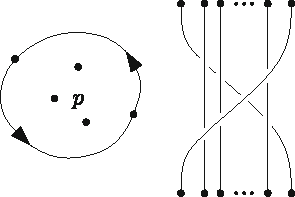
\includegraphics{img/interchange_loop_p.pdf}
  \caption{Exchange of a pair of Abelian $α$ anyons around $p$ fixed $α$ anyons. Figure taken from \cite{lundholm-solovej}.}
  \label{fig:abelian Up}
\end{figure}


\begin{proposition}[Ground state energy for a pair of Abelian anyons]
  Consider a pair of Abelian anyons with anyonic phase $\alpha$ enclosing $p$ fixed anyons (also with anyonic phase $\alpha$).
  The ground state energy is bound from below by
    \begin{gather*}
      \inf_{p,q\in\mathbb{Z}} \left(\alpha(1+2p)+2q\right)^2 =\\
      = \begin{cases}
        \frac{1}{\nu^2}, & \text{if $\alpha = \frac{\mu}{\nu}$ with $\mu \in \mathbb{Z}, \nu \in \mathbb{N}_+$ relatively prime and $\mu$ odd}, \\
        0, & \text{otherwise}
      \end{cases}
    \end{gather*}
\end{proposition}

\begin{proof}
  By \cref{eq:abelian Up} we have the anyonic exchange operator as
  \begin{align*}
    U_p = e^{i\alpha(1+2p)π}.
  \end{align*}
  By \cref{D spectrum} we have that the boundary condition gives
  \begin{align*}
    &u(π) = e^{i\alpha(1+2p)π} u(0) \\
    \iff\;\; &e^{iλ π} = e^{i\alpha(1+2p)π} \\
    \iff\;\; &λ = \alpha(1+2p) + 2q, \quad q \in \mathbb{Z}.
  \end{align*}
  Thus we see that the spectrum for $D$ and $H = D^2$, respectively, is
  \begin{align*}
    σ(D) &= \{ \alpha(1+2p) + 2q : q \in \mathbb{Z}\}, \\
    σ(H) &= \{ (\alpha(1+2p) + 2q)^2 : q \in \mathbb{Z}\}.
  \end{align*}
  Hence, the energy $λ^2$ is minimized for
  \begin{align*}
    E_0 = \inf_{p,q\in\mathbb{Z}} (\alpha(1+2p)+2q)^2.
  \end{align*}
  A number-theoretic result, found as proposition 5 in \cite{lundholm-solovej}, shows that this can be written as
  \begin{align*}
    E_0 =
    \begin{cases}
      \frac{1}{\nu^2}, & \text{if $\alpha = \frac{\mu}{\nu}$ with $\mu \in \mathbb{Z}, \nu \in \mathbb{N}_+$ relatively prime and $\mu$ odd}, \\
      0, & \text{otherwise}.
    \end{cases}
  \end{align*}
\end{proof}

From this we have an immediate corollary for bosons ($\alpha = 0$) and fermions ($\alpha = 1$).

\begin{corollary}
  With $\alpha = 0$, the anyonic phase reads
  \begin{align*}
    U_p = e^{i\alpha(1+2p)π} = 1
  \end{align*}
  for all $p$, i.e. bosons do not ``see'' each other, and they have a zero ground state energy.

  With $\alpha = 1$, the anyonic phase reads
  \begin{align*}
    U_p = e^{i\alpha(1+2p)π} = e^{i(1+2p)π},
  \end{align*}
  giving us the boundary condition
  \begin{align*}
    e^{iλ π} = e^{i(1+2p)π} &\iff λ = 1 + 2p + 2q, \quad q \in \mathbb{Z}
  \end{align*}
  Since $p$ is an integer, this shows that also fermions do not ``see'' the enclosed $p$ anyons.
  However, the anyons in the pair do ``see'' each other, in the sense that the their wave-function changes sign after they have been exchanged, as expected. Finally, this also shows that fermions have a non-zero ground state energy $E_0 = 1$.
\end{corollary}












\section{Non-Abelian anyons}

Consider the same setting as above, with the distinction that the anyons are now non-Abelian. That is, consider a pair of non-Abelian anyons, with wave-function $\psi \in L^2(\mathbb{R}; \mathbb{C}^n)$ parametrized by the relative angle $\varphi$, such that the pair of anyons encloses $p$ fixed anyons as $\varphi$ increases from $0$ to $π$, giving rise to an anyonic phase $U_p \in U(n)$.

% From \cref{D spectrum} the boundary condition reads
% \begin{align*}
%   u(π) = U_p u(0) \iff C e^{iλπ} = U_p C.
% \end{align*}
% This is precisely the condition that $e^{iλπ}$ is an eigenvalue of $U_p$.


% \hrule

% Consider first the case $n=2$, then $U_p \in U(2)$ can be parametrized as follows.

% \begin{lemma}[Characterization of $U(2)$ matrices]
%   Let $U \in U(2)$, then
%   \begin{align*}
%     U = \begin{pmatrix} a & b \\ -e^{i\thetaπ}\overline{b} & e^{i\thetaπ} \overline{a} \end{pmatrix}, \quad \operatorname{det} U = e^{i\thetaπ}.
%   \end{align*}
%   for $a,b,\theta \in \mathbb{R}$ such that $\abs{a}^2 + \abs{b}^2 = 1$ and $0 \le \theta < 2$.
%   The parameter $\theta$ corresponds to the Abelian phase in the factorization $U(2) = U(1)\times SU(2)$, where $\theta = 0$ gives $SU(2)$.
% \end{lemma}

% \hrule

A standard characterization of unitary matrices is as follows.

\begin{lemma}
  Let $U \in U(n)$, the $n$ eigenvalues (counted with multiplicity) of $U$ are on the form $e^{i\beta_jπ}$ for $j = 1,2,\ldots,n$. Furthermore, $e^{i\alpha\pi}$ where $\alpha = \frac{1}{n}\sum_j \beta_j$ is referred to as the Abelian phase of $U_p$. It is the Abelian part in the factorization of $U(n) = U(1) \times SU(n)$. Note that if $\det U = e^{iθπ}$ we have $α = θ/n$.
\end{lemma}

\begin{proof}
  We only show the $U(n) = U(1) \times SU(n)$ decomposition.
  Rewrite $U$ as $U = e^{i\alpha}\left( e^{-i\alpha} U \right)$ where $e^{i\alpha}$ is the Abelian part and $e^{-i\alpha} U$ is the $SU(n)$ part. It suffices to show that $\det \left( e^{-iαπ} U \right) = 1$,
  \begin{align*}
    \det \left( e^{-iαπ} U \right)
    &= \left(e^{-iαπ}\right)^n e^{i\left(\sum_j \beta_j\right)π} \\
    &= \left(e^{-i\left(\sum_j \beta_j\right)π/n}\right)^n e^{i\left(\sum_j \beta_j\right)π} = 1.
  \end{align*}
  On the other hand, $1 = \det \left( e^{-iαπ} U \right) = e^{-iαπn} e^{iθπ} = e^{i(-αn+θ)π}$, thus $α = θ/n$ (modulo $2$).
\end{proof}

Next, we show that the Abelian phase shifts the eigenvalues uniformly along the complex unit circle.

\begin{proposition}
  Consider non-Abelian anyons with arbitrary (unitary) $U_p \in U(n)$ exchange operator. The Abelian part of of the non-Abelian anyonic phase $U_p$ can always be chosen so that the ground state has zero energy.
\end{proposition}

\begin{proof}
  By changing the Abelian phase, each eigenvalue is shifted. This is obvious if we diagonalize $U_p$. In particular, adding $-\beta_j$ to the Abelian phase, the $j$:th eigenvalue is shifted to $e^{i(\beta_j-\beta_j)} = 1$, corresponding to zero energy.
\end{proof}

% From this, the Abelian part $e^{iαπ}$ of the anyonic phase $U_p \in U(n)$ can be seen as a shift of the eigenvalues $e^{iλπ}$ of $U_p$ along the complex unit circle, where $λ^2$ gives the energy of the system, as shown in figure \cref{fig: abelian phase shift}.

% \begin{figure}
%   \centering
%   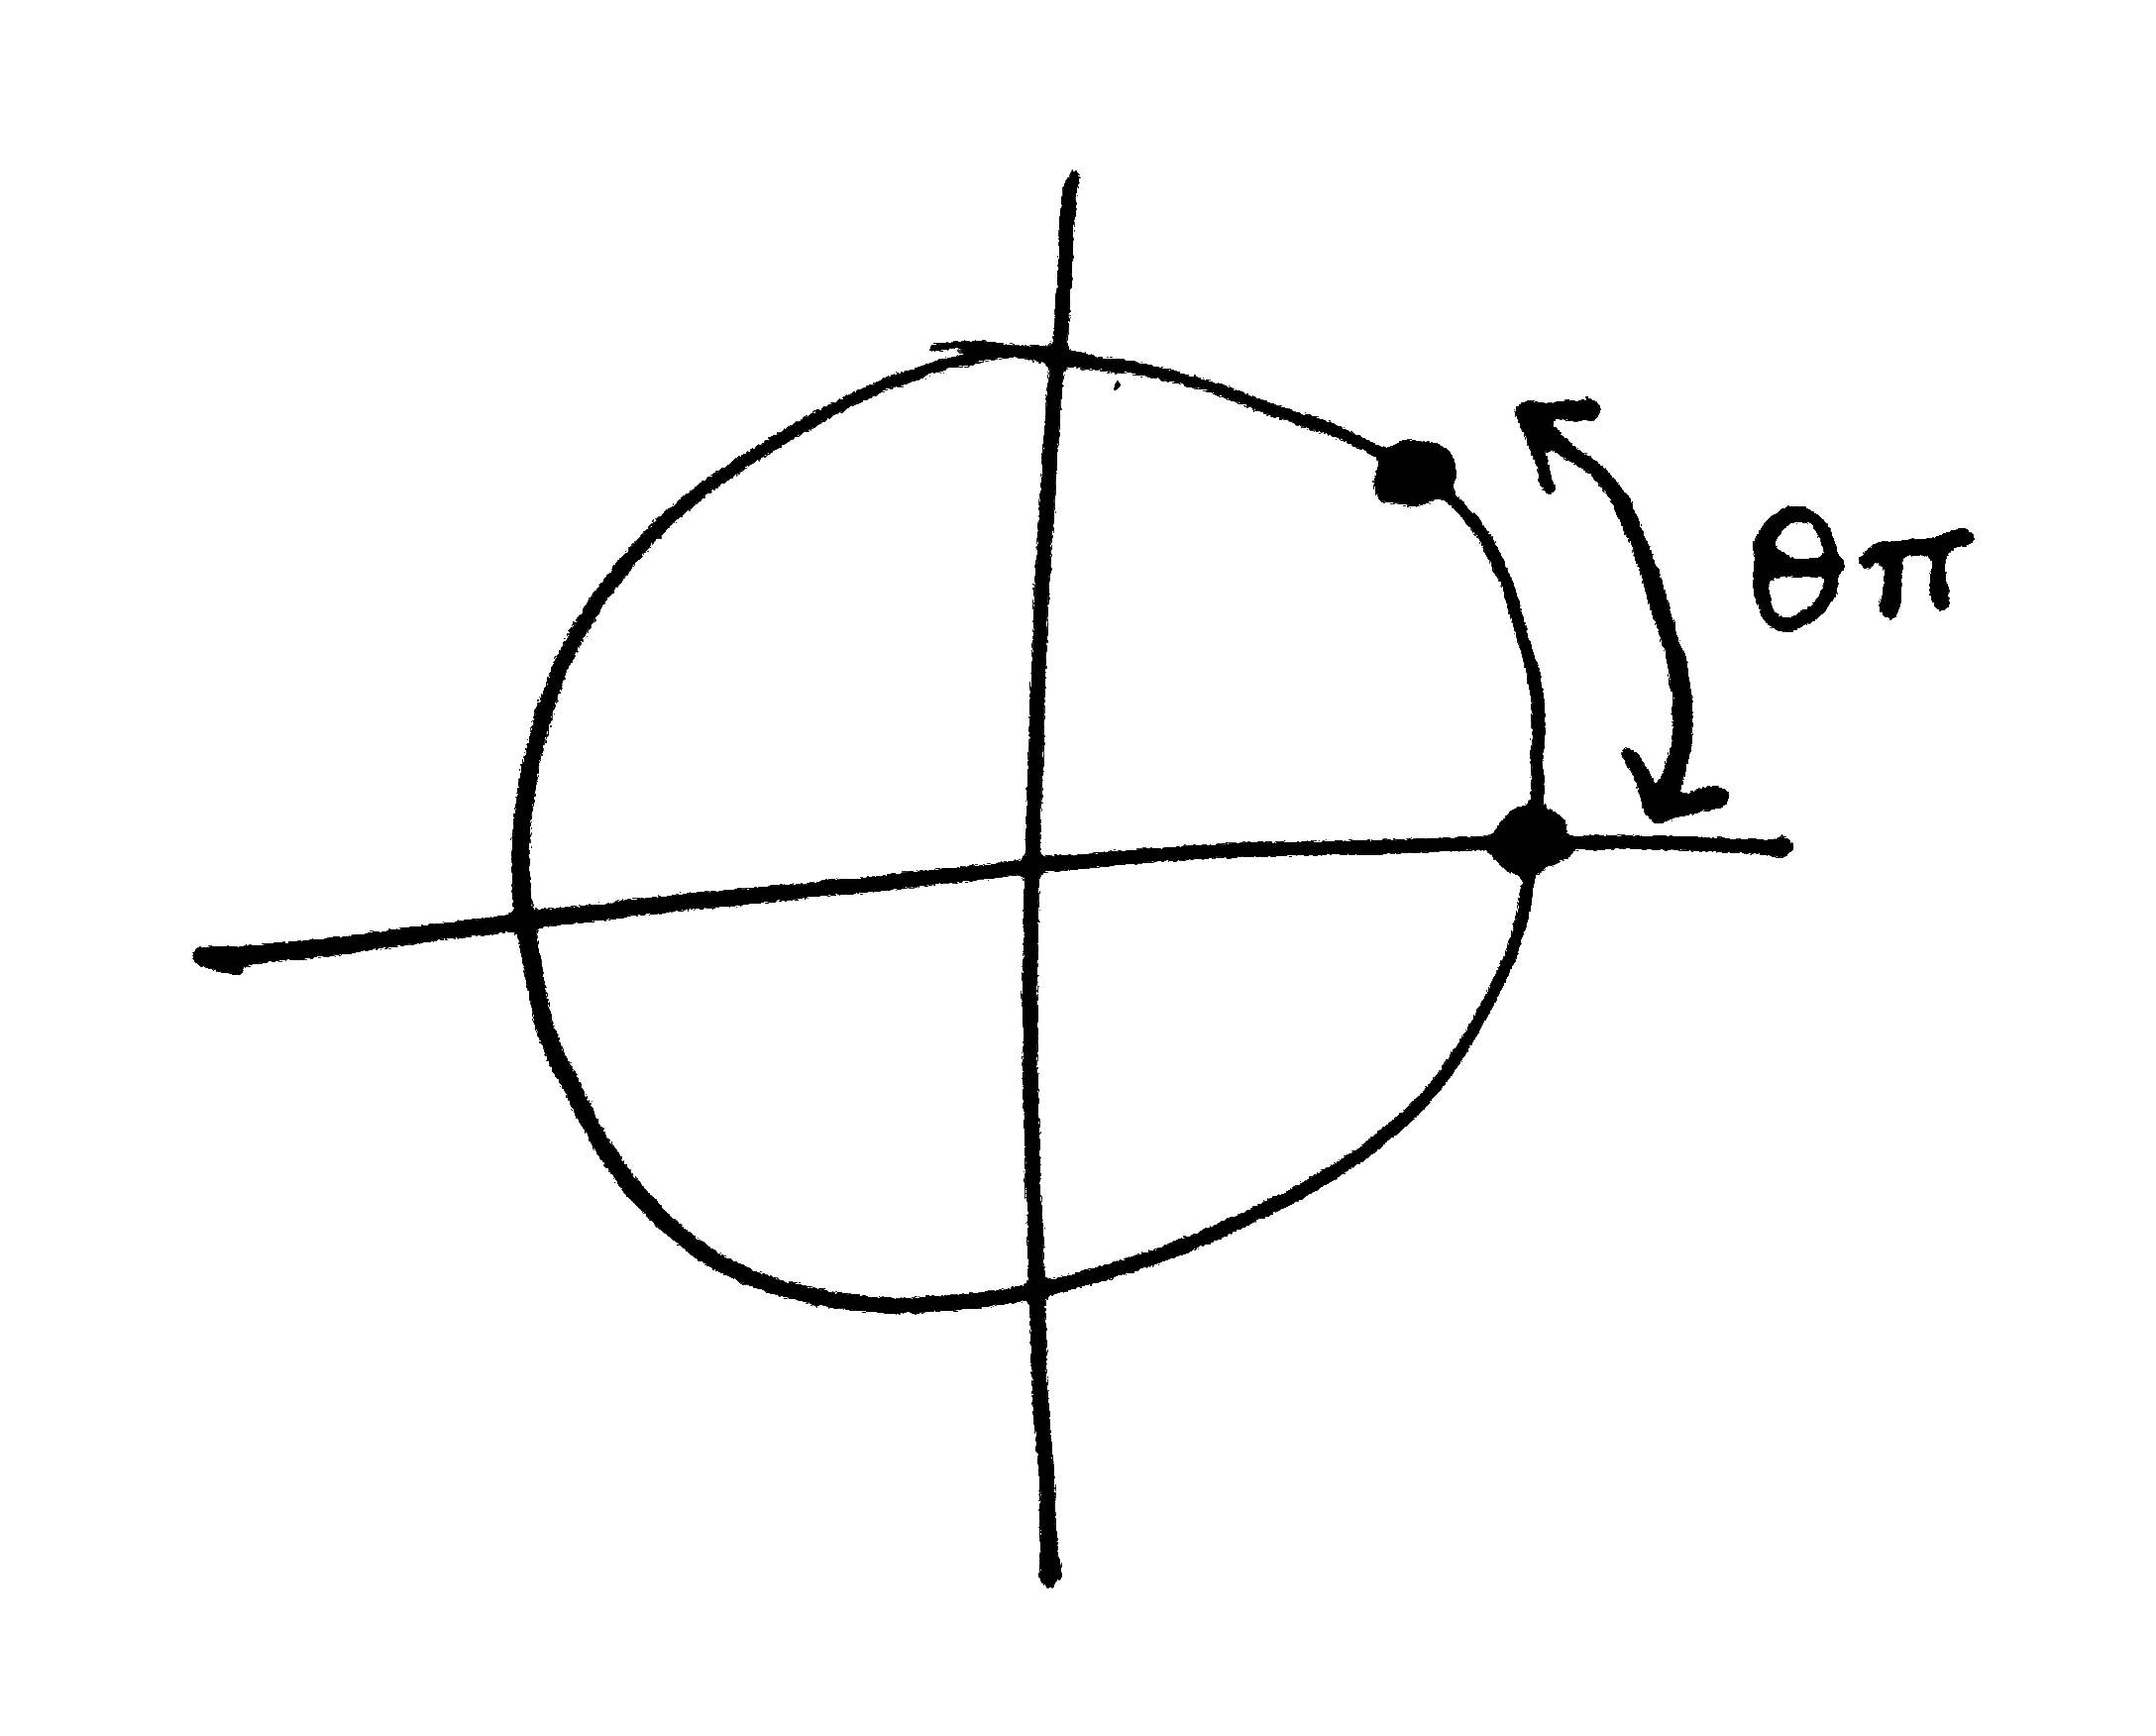
\includegraphics[width=0.5\linewidth]{img/abelian-phase-shift.jpg}
%   \caption{The shift of energy levels due to an Abelian phase $\alpha$ TODO it says theta.}
%   \label{fig: abelian phase shift}
% \end{figure}

As we shall see in the following chapter, the exchange operator $U_p$ has a rather involved dependence on the particular type of non-Abelian anyons that are considered. In order to characterize the energy bound, via the eigenvalues of $U_p$, we must first dive into the framework of abstract anyon models in order to characterize $U_p$.








































\chapter{Abstract anyon models}\label{anyon models}

In this chapter we shall present the framework of abstract anyon models, leading up to the succeeding chapter that characterizes braiding of anyons described abstract anyon models.

Anyon models can be modeled by unitary braided tensor categories, see \cite{kitaev,naaijkens}. However, setting up this framework in full generality is redundant for our purposes and we take a more straight forward approach, which is also most common in the literature. The benefit of the categorical approach is that consistency of braiding and fusion is most naturally shown this way. We shall see the ties between the straight forward approach and the categorical model in when discussing the consistency conditions in \cref{sec:pentagon hexagon}.

This chapter is in part based on \cite{preskill,kitaev,bonderson}. We shall be using the notation that is standard in the literature, and when possible make use of and extend the fusion diagram notation, which greatly clarifies braiding of fusion states.

Starting with \cref{sec:anyonic braid representations in fusion space} we show how a given abstract anyon model gives rise to representations of the braid group.

\section{Preliminaries}

An abstract anyon model consists of a set of labels representing different types of anyons. These labels are known as anyonic charge, topological charge or superselection labels. Anyons can be combined, or fused, to give an anyon of some charge, possibly in different ways. This is modeled by a fusion algebra
\begin{align*}
  a \times b = \sum_c N_{ab}^c c
\end{align*}
representing the possible outcomes from fusion of anyons of type $a$ and $b$. The fusion multiplicities $N_{ab}^c$ are non-negative integers denoting the number of distinct ways $a$ and $b$ can fuse to $c$. In each anyon model there is the trivial label $1$, representing the vacuum, with the property $N_{a1}^b = N_{1a}^b = \delta_{ab}$, i.e. $1$ fuses trivially with every other charge. Furthermore, to each charge $a$ there is a corresponding conjugate charge $\bar{a}$ representing the antiparticle of $a$, with the property $N_{ab}^1 = \delta_{b\bar{a}}$, i.e. $a$ fuses to the vacuum only with its antiparticle.

% Fusion of $a$ and $b$ is given by $a \times b = \sum_c N_{ab}^c c$

% The state space of anyons resulting from fusion of anyons $a_1, \ldots, a_n$ is denoted by $V_{a_1 \ldots a_n}$ and can be decomposed as
% \begin{align*}
%   V_{a_1 \ldots a_n} = \bigoplus_b = V_{a_1 \ldots a_n}^b
% \end{align*}
% where $V_{a_1 \ldots a_n}^b$ denotes the state space of anyons of type $b$ resulting from fusion of $a_1, \ldots, a_n$.

The $N_{ab}^c$ distinguishable ways in which $a$ and $b$ can fuse to $c$ can be regarded as an orthonormal basis of a Hilbert space $V_{ab}^c$. This is the state space, or fusion space, of anyons of type $c$ resulting from fusion of $a$ and $b$. The states of $V_{ab}^c$ are called fusion states and we denote the basis for $V_{ab}^c$ by
\begin{align*}
  \{ \ket{ab;c,\mu}, \quad \mu = 1,2,\ldots,N_{ab}^c \}
\end{align*}
where $\ket{ab;c,\mu}$ represents the $\mu$:th way in which $a$ and $b$ can fuse to $c$. This is the notation used by \cite{preskill}.

The splitting space $V_c^{ab}$ is the dual space of the fusion space $V_{ab}^c$, it is the state space of particles with anyonic charge $a$ and $b$ that can be split from an anyon of charge $c$.

More generally, the fusion space of anyons of type $c$ resulting from fusion of anyons of type $a_1, \ldots, a_n$ is denoted by $V_{a_1 a_2 \cdots a_n}^c$. This space has a canonical decomposition
\begin{align*}
  V_{a_1 a_2 \cdots a_n}^c \cong \bigoplus_{b_1,b_2,\ldots,b_{n-2}} V_{a_1a_2}^{b_1} \otimes V_{b_1 a_3}^{b_2} \otimes V_{b_2 a_4}^{b_3} \ldots \otimes V_{b_{n-2} a_n}^c
\end{align*}
with an associated canonical orthonormal basis with elements being the fusion states
\begin{align*}
  \ket{a_1 a_2; b_1, \mu_1} \otimes \ket{b_1 a_3; b_2, \mu_2} \otimes \cdots \otimes \ket{b_{n-3} a_{n-1}; b_{n-2}, \mu_{n-2}} \otimes \ket{b_{n-2} a_n; c, \mu_{n-1}}
\end{align*}
for all possible $b_j$ and $\mu_j$. For convenience we write $b_{0} = a_1$ and $b_{-1} = 1$.

Many anyon models of interest have the property that $N_{ab}^c \le 1$ for all particle types $a, b$ and $c$. When this is the case, such as for the Fibonacci anyons that we shall consider in \cref{fibonacci anyons}, the multiplicity label $\mu$ can be ignored. This makes the model easier to handle, and we introduce the fusion diagram notation.


\section{Fusion diagrams}

In the previous section we defined
\begin{align*}
  \ket{ab;c,μ}
\end{align*}
to represent the $μ$:th way in with $a$ and $b$ fuse to $c$. It shall be very convenient to use a diagrammatic notation for fusion states when considering braiding of anyons, as we shall see in the following sections. Thus, we introduce the notation
\begin{align*}
  \begin{tikzpicture}[scale=0.4,font=\footnotesize,anchor=mid,baseline={([yshift=-.5ex]current bounding box.center)}]
    \node at (0, 1.7) {$b$};
    \draw (0, 1.4) to (0, 0.45);
    \draw (-1.5, 0) to (-0.45, 0);
    \draw (0.45, 0) to (1.5, 0);
    \draw (0, 0) circle (0.45);
    \node at (0.003, 0.08) {$\mu$};
    \node at (-1.2, -0.4) {$a$};
    \node at (1.2, -0.4) {$c$};
  \end{tikzpicture}
  \coloneqq \ket{ab;c;\mu}
\end{align*}
Note that the diagram should be read left/top to right/bottom, i.e.\ $a$ fuses with $b$ resulting in $c$.
For simplicity we suppress the multiplicity label $\mu$ in the notation and write
\begin{align*}
  \fs{b}{a,c} \coloneqq
  \begin{tikzpicture}[scale=0.4,font=\footnotesize,anchor=mid,baseline={([yshift=-.5ex]current bounding box.center)}]
    \node at (0, 1.7) {$b$};
    \draw (0, 1.4) to (0, 0.45);
    \draw (-1.5, 0) to (-0.45, 0);
    \draw (0.45, 0) to (1.5, 0);
    \draw (0, 0) circle (0.45);
    \node at (0.003, 0.08) {$\mu$};
    \node at (-1.2, -0.4) {$a$};
    \node at (1.2, -0.4) {$c$};
  \end{tikzpicture}
  \coloneqq \ket{ab;c;\mu}.
\end{align*}
This is convenient, since most models we shall consider are such that the fusion multiplicities are trivial, $N_{ab}^c \le 1$. That is, if fusion of $a$ and $b$ to $c$ is possible, this happens in exactly one way. Then, the multiplicity label $\mu$ in $\ket{ab;c,\mu}$ can be ignored, because the only possibility is $\mu = 1$, if $\mu=0$ the state is not valid. This is not a major simplification in the notation, it shall always be straight forward to add back the multiplicity labels if needed.

The diagram notation is primarily useful when considering fusion of several anyons and extends in a natural way;
\begin{align*}
  \fs{b,c}{a,e,d}
\end{align*}
denotes fusion of $a,b,c$ to $d$ such that $a$ fuses with $b$ resulting in the intermediate charge $e$, finally $e$ fuses with $c$ to give the resulting charge $d$.

The canonical basis for the fusion space $V_{a_1a_2\cdots a_n}^c$ with canonical decomposition
\begin{align*}
  V_{a_1 \cdots a_n}^c \cong \bigoplus_{b_1,b_2,\ldots,b_{n-2}} V_{a_1a_2}^{b_1} \otimes V_{b_1 a_3}^{b_2} \otimes V_{b_2 a_4}^{b_3} \ldots \otimes V_{b_{n-2} a_n}^c
\end{align*}
can thus be written in terms of fusion diagrams, assuming trivial fusion multiplicities, as
\begin{align*}
  \left\{
  \begin{tikzpicture}[scale=0.3,font=\footnotesize,anchor=mid,baseline={([yshift=-.5ex]current bounding box.center)}]
    \node at (0, -0.6) {$a_1$};
    \node at (1, 2) {$a_2$};
    \node at (3, 2) {$a_3$};
    \node at (10, 2) {$a_{n-1}$};
    \node at (13, 2) {$a_n$};
%
    \draw (1, 0) to (1, 1.5);
    \draw (3, 0) to (3, 1.5);
%
    \draw (10, 0) to (10, 1.5);
    \draw (13, 0) to (13, 1.5);
%
    \draw (-1, 0) to (5, 0);
    \draw (7, 0) to (15, 0);
%
    \node at (2, -0.7) {$b_1$};
    \node at (4, -0.7) {$b_2$};
    \node at (6, 0.2) {$\cdots$};
%
    \node at (8.5, -0.7) {$b_{n-3}$};
    \node at (11.5, -0.7) {$b_{n-2}$};
    \node at (14, -0.7) {$c$};
  \end{tikzpicture}
  \;\;\;\bigg|\; \begin{array}{c}\text{for all possible intermediate} \\ \text{charges $b_1, b_2, \ldots, b_{n-2}$}\end{array}
  \right\}.
\end{align*}
It is thus clear that for given anyons $a_1, \ldots, a_n$ the fusion states are really determined by the intermediate charges $b_j$.

The real advantage of writing fusions states with fusion diagrams is that braiding is much easier to represent. This will be extremely useful now as we proceed in developing the abstract model for anyons, and characterize braiding.

Consider an arbitrary fusion state $\ket{\psi} = \sum_k c_k \ket{k}$ where $\ket{k}$ denotes the $k$:th basis fusion states. Let $A$ be a linear operator on the fusion space. The basis fusion states are transformed according to
\begin{equation}\label{eq:linear op on basis state}
  A\ket{k} = \sum_j A_{jk} \ket{j}
\end{equation}
The action of a linear operator $A$ acting on $\ket{\psi}$ is then given by
\begin{equation}
  A \ket{\psi} = \sum_k c_k A \ket{k} = \sum_{k} c_k \sum_j A_{jk} \ket{j} = \sum_j \sum_k c_k A_{jk} \ket{j}.
\end{equation}

In what follows, we shall define some important linear operators. We shall define the operators in terms of their action on the on the standard fusion states, as in \cref{eq:linear op on basis state}.












\section{The $F$ operator: Associativity of fusion}

The result of fusing multiple anyons must be independent of which anyons are fused first. That is, fusion is associative,
\begin{align*}
  (a \times b) \times c = a \times (b \times c)
\end{align*}
This gives rise to a natural isomorphism between the two decompositions of the fusion space
\begin{align*}
  V_{abc}^d \cong
  \bigoplus_f V_{ab}^f \otimes V_{fc}^d
  \cong
  \bigoplus_e V_{bc}^e \otimes V_{ae}^d
  .
\end{align*}
The first decomposition should be understood as first fusing $a$ with $b$ in all possible ways giving an intermediate charge $f$, followed by fusing $c$ with $f$ to give the final charge $d$.
The second decomposition should be understood as first fusing $b$ with $c$ in all possible ways giving an intermediate charge $e$, followed by fusing $a$ with $e$ to give the final charge $d$.

The first of these two decompositions is referred to as the standard decomposition and the second is the fusion decomposition. We denote this isomorphism by
\begin{align*}
  F : \bigoplus_f V_{ab}^f \otimes V_{fc}^d \to \bigoplus_e V_{bc}^e \otimes V_{ae}^d
\end{align*}
and it can be represented by the $F$ matrix.

\begin{definition}
  The $F$ matrix $F_{abc}^c$ is given by
  \begin{equation}\label{F-matrix}
    F : \fs{b,c}{a,e,d} \mapsto \fsfused{a}{b}{c}{d}{e} = \sum_f \left(F_{abc}^d\right)_{fe} \fs{b,c}{a,f,d}.
  \end{equation}
\end{definition}

That is, the $F$-matrix is the change of basis matrix from the standard basis to the fused basis in the fusion space $V_{abc}^d$.

\begin{remark}[Implicit range for the index of summation]\label{rem:sum index range}
  In \cref{F-matrix} the summation index $f$ implicitly ranges over all possible labels in the given anyon model, with the obvious restriction that the corresponding fusion state in the summand is valid. That is, the summation index $f$ must be such that
  \begin{align*}
    a \times b &= f \\
    f \times c &= d.
  \end{align*}
  Similarly, the label $e$ is restricted so that
  \begin{align*}
    b \times c &= e \\
    a \times e &= d.
  \end{align*}
  In what follows we shall let the summation index be implicit in all sums with fusion states as summands.
\end{remark}

The following lemma will be useful when computing the $F$-matrix.

\begin{lemma}\label{res:F1}
  Consider the fusion space $V_{abc}^d$, when one of the particle types is trivial, i.e. $a,b,c$ or $d$ equals $1$, then $\dim V_{abc}^d = 1$ and the corresponding $F$-matrix $F_{abc}^d$ is trivial. More explicitly we have
  \begin{align*}
    F_{1bc}^d &= \left( F_{1bc}^d \right)_{bd} = 1, \\
    F_{a1c}^d &= \left( F_{a1c}^d \right)_{ac} = 1, \\
    F_{ab1}^d &= \left( F_{ab1}^d \right)_{db} = 1, \\
    F_{abc}^1 &= \left( F_{abc}^1 \right)_{\overline{c}\,\overline{a}} = 1.
  \end{align*}
\end{lemma}

\begin{proof}
  With $a = 1$ we have, by definition of the $F$-matrix,
  \begin{align*}
     \fsfused{1}{b}{c}{d}{e} = \sum_f \left(F_{1bc}^d \right)_{fe} \fs{b,c}{1,f,d}.
  \end{align*}
  From the fusion diagram on the right hand side we read out $1 \times b = f$ from the first fusion, this is valid only for $f = b$.
  Similarly, on the left hand side the final fusion reads $1 \times e = d$, implying $e = d$. Since the indices $e$ and $f$ are forced, this implicitly shows that the corresponding fusion spaces is one-dimensional. The other results follow analogously,
  \begin{align*}
    % \fs{b,c}{a,e,d} &= \sum_f \left(F_{abc}^d \right)_{ef} \fsfused{a}{b}{c}{d}{f} \\
    \fsfused{a}{1}{c}{d}{e} &= \sum_f \left(F_{a1c}^d \right)_{fe} \fs{1,c}{a,f,d} \implies e = c, f = a, \\
    \fsfused{a}{b}{1}{d}{e} &= \sum_f \left(F_{ab1}^d \right)_{fe} \fs{b,1}{a,f,d} \implies e = b, f = d, \\
    \fsfused{a}{b}{c}{1}{e} &= \sum_f \left(F_{abc}^1 \right)_{fe} \fs{b,c}{a,f,1} \implies e = \overline{a}, f = \overline{c}.
  \end{align*}
  The result can also be realized by noting that three anyons of type $a, b$ and $c$, where one of them is the trivial type $1$, is uniquely determined by their total charge. Indeed, these three anyons are really just two, since the trivial particle $1$ fuses trivially, it can be added or removed in the representation without changing anything. Thus, the corresponding $F$ matrix must be trivial in this case. This is particularly clear if $b$ or $c$ equals $1$, we then have
  \begin{align*}
    \fsfused{a}{1}{c}{d}{e} = \fsfused{a}{1}{c}{d}{c} = \fs{c}{a,d}
  \end{align*}
  and it is clear that no fusion can occur.
\end{proof}















\section{The $R$ operator: Commutativity of fusion}

The result of fusing $a$ with $b$ must be the same as fusing $b$ with $a$. That is, fusion is commutative,
\begin{align*}
  a \times b = b \times a.
\end{align*}
This gives rise to a natural isomorphism
\begin{align*}
  R : V_{ba}^c \to V_{ab}^c
\end{align*}
between the corresponding fusion spaces which can be represented by a unitary matrix $R_{ab}^c$ acting on the fused basis states
\begin{align*}
  \fsfused{}{a}{b}{}{c}.
\end{align*}
\begin{definition}
  The $R$ matrix $R_{ab}$ is given by
  \begin{equation}\label{R-matrix}
    R : \fsfused{}{a}{b}{}{c} \mapsto \fsfusedbraided{}{a}{b}{}{c} = R_{ab}^c \fsfused{}{a}{b}{}{c}.
  \end{equation}
\end{definition}
It is clear that $R$-matrix $R_{ab}$ is diagonal and we can denote this as
\begin{align*}
  (R_{ab})_{ij} = \delta_{ij} R_{ab}^i.
\end{align*}













\section{The $B$ operator: Braiding of standard fusion states}

We shall now consider braiding on the standard fusion states. This can be realized by applying the $F$-matrix to put the state in a basis where the $R$ matrix can be applied immediately, followed by reverting back to the standard basis via $F^{-1}$. That is, using the $F$ and $R$-matrix we obtain the relation
% \begin{align*}
%   \fs[1]{b,c}{a,e,d}
%   &= \sum_f \left(F_{acb}^d\right)_{ef} \fsfusedbraided{a}{b}{c}{d}{f} \\
%   &= \sum_f \left(F_{acb}^d\right)_{ef} R_{bc}^f \fsfused{a}{b}{c}{d}{f} \\
%   &= \sum_g \sum_f \left(F_{acb}^d\right)_{ef} R_{bc}^f \left((F^{-1})_{abc}^d\right)_{fg} \fs{b,c}{a,g,d}.
% \end{align*}
\begin{align*}
  \fs[1]{b,c}{a,e,d}
  &= \sum_f \left(\left(F^{-1}\right)_{acb}^d\right)_{fe} \fsfusedbraided{a}{b}{c}{d}{f} \\
  &= \sum_f \left(\left(F^{-1}\right)_{acb}^d\right)_{fe} R_{bc}^f \fsfused{a}{b}{c}{d}{f} \\
  &= \sum_g \sum_f \left(\left(F^{-1}\right)_{acb}^d\right)_{fe} R_{bc}^f \left(F_{abc}^d\right)_{gf} \fs{b,c}{a,g,d}.
\end{align*}
Recall the implicit summation index convention described in \cref{rem:sum index range}.
From this we define the $B$-matrix.
\begin{definition}\label{def:B}
  The $B$ matrix $B_{abc}^d$ is given by
  \begin{align*}
    \left(B_{abc}^d\right)_{eg} = \sum_f \left(\left(F^{-1}\right)_{acb}^d\right)_{ef} R_{bc}^f \left(F_{abc}^d\right)_{fg}.
  \end{align*}
  Symbolically we write this as
  \begin{align*}
    B = F^{-1} R F.
  \end{align*}
\end{definition}
To sum up, the $B$-matrix braids the standard fusion states according to
\begin{align*}
  \fs[1]{b,c}{a,e,d} = \sum_g \left(B_{abc}^d\right)_{ge} \fs{b,c}{a,g,d}.
\end{align*}

As a consequence of the definition of the $B$-matrix and \cref{res:F1} we have the following lemma, which will be useful when computing the $B$-matrix.

\begin{lemma}\label{res:B1}
  Consider the fusion space $V_{abc}^d$, when one of the particle types is trivial, i.e. $a,b,c$ or $d$ equals $1$, then $\dim V_{abc}^d = 1$ and the corresponding $B$-matrix $B_{abc}^d$ is one-dimensional,
  \begin{align*}
    B_{1bc}^d &= \left( B_{1bc}^d \right)_{bc} = R_{bc}^d, \\
    B_{a1c}^d &= \left( B_{a1c}^d \right)_{ad} = R_{1c}^c = 1, \\
    B_{ab1}^d &= \left( B_{ab1}^d \right)_{da} = R_{b1}^b = 1, \\
    B_{abc}^1 &= \left( B_{abc}^1 \right)_{\overline{c}\,\overline{b}} = R_{bc}^{\overline{a}}.
  \end{align*}
\end{lemma}















































\section{The pentagon and hexagon equations}\label{sec:pentagon hexagon}

When considering an anyon model, it is ultimately the $B$ operator (braid operator) that describes how braiding affects the anyons. The $B$ operator gives the phase change introduced when braiding anyons. In the next chapter we shall explicitly see how the $B$ operator is used to characterize the braid group representation for anyon models. It is the braid group representation that is the relevant property both for the study the dynamics of anyons, but also for developing methods for quantum computation with anyons, known as topological quantum computation.

We have seen that the $B$-matrix is computed from the $F$ and $R$-matrices. These matrices are in turn determined by what is known as the pentagon equation
\begin{equation}\label{eq:pentagon}
  \left(F_{12c}^5\right)^d_a \left(F_{a34}^5\right)^c_b = \left(F_{234}^d\right)_c^c \left( F_{1e4}^5 \right)^d_b \left( F_{123}^b \right)^e_a
\end{equation}
and hexagon equation
\begin{equation}\label{eq:hexagon}
  % R_{13}^c \left(F_{213}^4\right)^c_a R_{12}^a = \sum_{b} \left(F_{231}^4\right)^c_b R_{1b}^4 \left(F_{123}^4\right)^b_a.
  R_{ac}^g \left(F_{bac}^d\right)^g_e R_{ab}^e = \sum_{f} \left(F_{bca}^d\right)^g_f R_{af}^d \left(F_{abc}^d\right)^f_e.
\end{equation}
In these equations, all indices are taken as arbitrary particle labels.

These equations should be understood as coherence conditions for fusion and braiding. The diagrammatic version of these equations, found as commutative diagrams in \cref{fig:pentagon_diagram,fig:hexagon_space} and \cref{fig:pentagon_space,fig:hexagon_space} make the point clear, and shows that these equations are commutativity constraints for fusion and braiding. Indeed, the pentagon equation is the formal constraint for associativity of fusion,
\begin{align*}
  (a \times b) \times c = a \times (b \times c).
\end{align*}
As previously hinted, anyon models can be described by braided tensor categories. In this setting, the pentagon and hexagon equations are precisely Mac Lane's coherence theorem \cite{mac lane}, showing that no further conditions are required for consistent fusion and braiding. Further details can be found in \cite{kitaev,preskill}.

Solving the pentagon and hexagon equations is in general highly non-trivial. The equations are multivariate polynomial equations and require elaborate techniques to be solved. First one must fix the gauge freedom that comes from the choice of basis for the fusion space, next an appropriate Gröbner basis can be used to solve the system. See \cite{bonderson} for more details on this approach.

\begin{figure}[h]
  \centering
  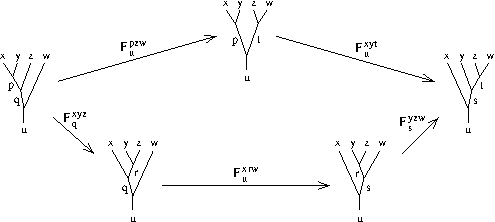
\includegraphics[width=1\linewidth]{img/pentagon_diagram.pdf}
  \caption{The pentagon equation in terms of fusion diagrams. Figure take from \cite{kitaev}. Note that the $F$-matrix have super- and sub-scripts reversed.}
  \label{fig:pentagon_diagram}
\end{figure}

\begin{figure}[h]
  \centering
  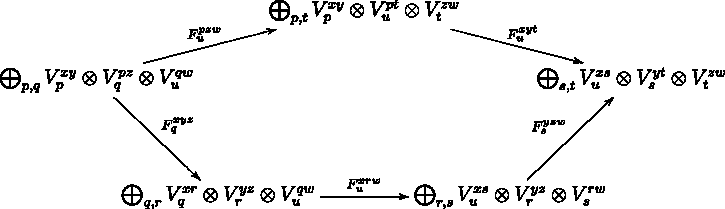
\includegraphics[width=1\linewidth]{img/pentagon_space.pdf}
  \caption{The pentagon equation in terms of fusion spaces. Figure take from \cite{kitaev}. Note that the fusion spaces and the $F$-matrix have super- and sub-scripts reversed.}
  \label{fig:pentagon_space}
\end{figure}

\begin{figure}[h]
  \centering
  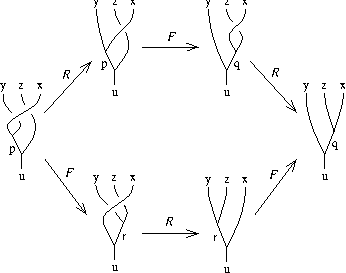
\includegraphics[width=0.8\linewidth]{img/hexagon_diagram.pdf}
  \caption{The hexagon equation in terms of fusion diagrams. Figure take from \cite{kitaev}.}
  \label{fig:hexagon_diagram}
\end{figure}

\begin{figure}[h]
  \centering
  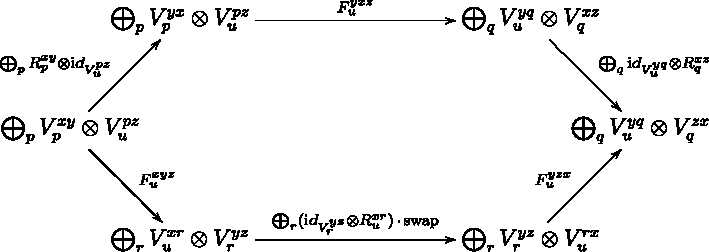
\includegraphics[width=1\linewidth]{img/hexagon_space.pdf}
  \caption{The hexagon equation in terms of fusion spaces. Figure take from \cite{kitaev}. Note that the fusion spaces, $F$-matrix and $R$-matrix have super- and sub-scripts reversed.}
  \label{fig:hexagon_space}
\end{figure}


\clearpage






































































\chapter{Anyonic braid group representations}

In this chapter we show how a given anyon model gives rise to representations of the braid group. The chapter builds up to a general characterization of the exchange operator $U_p$ of a pair of anyons around $p$ enclosed anyons. To give a detailed account of exactly how the representations of the braid group generators arise, we begin by defining charge sectors of fusion spaces.


\section{Charge sectors}\label{sec:charge sectors}

Consider any abstract anyon model with a non-trivial particle label $t$. When considering braiding of two intermediate $t$ anyons in $V_{t^n}^1$, it suffices to work with the basis of $V_{t^n}^1$ restricted to the intermediate charge labels $a,b$ and $c$ in
\begin{align*}
  \cdots \fs{t,t,\bm{t},\bm{t},t,t}{\cdot,\cdot,a,b,c,\cdot,\cdot} \cdots
\end{align*}
The reason for this is that only these labels are part of the $B$ matrix describing braiding of the two $t$ anyons.
Note that we cannot make any assumptions for the charge $c$, it is not forced to be $1$ since we are considering intermediate anyons in the fusion space, only the total charge of the fusion space is specified, in this case $1$. The different possible values for $c$ is referred to as different right charge sector. Similarly, also the charge $a$ is unknown, because we are not considering the leftmost particle in the basis, there are really more anyons to the left, that fuse to different resulting charges $a$. This results in different left charge sectors.

If we fix the both the left and right charge sectors to be trivial, we are really considering braiding of
\begin{align*}
  \fs{t,t}{1,b,1}
\end{align*}
in $V_{tt}^1$. This is a different fusion space, with much smaller dimension than $V_{t^n}^1$. There is just one free intermediate charge label here, compared to three free charge labels when not fixing the charge sectors.

Note that having trivial total charge, as in $V_{t^n}^1$ represents the fact that we have exactly $n$ anyons of type $t$. If the total charge would be $t$, there would really be $n+1$ anyons of type $t$ available.

% TODO: Can this be used?
% As an example of the importance of the charge sectors, considering braiding of the last pair of anyons. Then, the charge sector is known, it must be $1$, the total charge of the fusion space $V_{t^n}^1$. This allows for a straight-forward computation of $ρ(σ_{n-1})$, as shown in \cref{res:sigma n-1 is R}. Similarly, the left charge sector of $ρ(σ₁)$ is $1$, c.f.\ \cref{res:sigma 1 is R}.

Since we seek to characterize general braiding in $V_{t^n}^1$, including intermediate anyons where both the left and right charge sector are unfixed, we introduce the following definition for convenience.

\begin{definition}\label{def:full fusion space}
  The fusion space $\widetilde{V}_{t^n}$ has basis elements on the form
  \begin{align*}
    \fswide{t,t}{b_1,b_2,b_3}
    \cdots
    \fswide{t,t}{b_{n-1},b_n,b_{n+1}}
  \end{align*}
  where the charge labels $b_1, b_2, \ldots, b_{n+1}$ range over all values allowed by the fusion rules. The space $\widetilde{V}_{t^n}$ should be thought of as the space $V_{t^n}^1$ but including all possible left and right charge sectors. That is, the space of $n$ anyons of type $t$ with unfixed charge sectors.
\end{definition}

The following new notation shall be convenient when working with such fusion spaces.

\begin{definition}
  The basis fusion states of the fusion space $\widetilde{V}_{t^n}$ are denoted
  \begin{align*}
    \ket{b_1 b_2 \cdots b_{n} b_{n+1}} \coloneqq
    \fswide{t,t}{b_1,b_2,b_3}
    \cdots
    \fswide{t,t}{b_{n-1},b_n,b_{n+1}},
  \end{align*}
  where the $n$ anyons of type $t$ are implicit in this notation.
\end{definition}

\begin{remark}
  We now have three slightly different notations for fusion spaces, to sum up:
  \begin{align*}
    V_{t^n}^1 &: =
    \operatorname{span} \left\{ \fswide{t,t}{\bm{1},t,b_1} \cdots \fswider{t,t}{b_{n-3},b_{n-2},\bm{1}} : \text{ for all possible $b_j$} \right\} \\
    V_{t^n} &: =
    \operatorname{span} \left\{ \fswide{t,t}{\bm{1},t,b_1} \cdots \fswider{t,t}{b_{n-3},b_{n-2},\bm{b_{n-1}}} : \text{ for all possible $b_j$} \right\} \\
    \widetilde{V}_{t^n} &: =
    \operatorname{span} \left\{ \fswide{t,t}{\bm{b_1},b_2,b_3} \cdots \fswider{t,t}{b_{n-1},b_n,\bm{b_{n+1}}} : \text{ for all possible $b_j$} \right\}
  \end{align*}
  Note how the only thing that differs are the left and right charge sectors.
  Recall the notation $V_{t^n} = \bigoplus_c V_{t^n}^c$, this is the space of $n$ anyons of type $t$ with free right charge sector.
\end{remark}

We shall now see how braid group representations arise in the fusion space $\widetilde{V}_{t^n}$ for given non-trivial anyonic charge $t$. We let the left and right charge sectors be unspecified, meaning that the $n$ anyons we consider may really be part of a larger ensemble of anyons. If we in total had exactly $n$ anyons, it would suffice to consider the fusion space $V_{t^n}^1$, i.e.\ with left and right charge sectors fixed to $1$, but we proceed without this restriction. Note that we could instead consider the more general fusion space $\widetilde{V}_{a_1 \cdots a_n}$, however one is most often interested in braiding of anyons of the same type. This is also exactly what we need for the purposes outlined in \cref{chap:kinetic energy}. The fusion space $\widetilde{V}_{a_1 \cdots a_n}$ is treated analogously to $\widetilde{V}_{t^n}$.






















\section{Braid group representations in \texorpdfstring{$\widetilde{V}_{t^n}$}{V\~_(τⁿ)}}\label{sec:anyonic braid representations in fusion space}

Each anyon model gives rise to representations of the braid group, the representations depend on the number of considered anyons and the possible charges sectors. In this and the following sections we give a detailed account of how braid group representations comes about in the framework of abstract anyon models. An account of the general theory of braid group representations, not necessarily arising from abstract anyon models, can be found in \cite{oskar}.

Single out a non-trivial anyonic charge and consider the fusion space $\widetilde{V}_{t^n}$ with the standard basis. In this space we naturally have $n-1$ braid group generators by exchanging neighbouring $t$ anyons, we introduce the following notation.

\begin{definition}\label{def:rho_n sigma_j}
  The representation of the $j$:th braid group generator $σ_j$ in $\widetilde{V}_{t^n}$ is denoted $ρ_n(σ_j)$.
\end{definition}

For example, we have
\begin{align*}
  \fswide{t,t}{\cdot,\cdot,\cdot} \xmapsto{\rho_2(\sigma_1)} \fswide[1]{t,t}{\cdot,\cdot,\cdot}
\end{align*}
this is precisely the $B$ operator
\begin{align*}
  B : \fswide{t,t}{b_1,b_2,b_3} \mapsto \fswide[1]{t,t}{b_1,e,b_3} =
  \sum_{b_2} \left( B_{b_1tt}^{b_3} \right)_{b_2 e} \fswide{t,t}{b_1,b_2,b_3}.
  % \rho_2(\sigma_1)\left(\fswide{t,t}{b_1,b_2,b_3}\right)
\end{align*}
This shows that $ρ_2(σ_1)$ in $\widetilde{V}_{t^2}$ for fixed $b_1$ and $b_3$ is given by
\begin{align*}
  ρ_2(σ_1) = \bigoplus_{b_1, b_3} B_{b_1tt}^{b_3}.
\end{align*}
By the definition of the $B$ matrix we see that there is no mixing of the values for $b_1$ or $b_3$, this matrix really only acts on the subspace generated by the possible values of the label $b_2$ while keeping the labels $b_1$ and $b_3$ fixed.

% , denoted $\ket{b_1 [b_2], b_3}$.
% We write this as
% TODO FIX NOTATION
% \begin{align*}
%   ρ_2(σ_1) \left( \fswide{t,t}{b_1,\langle b_2 \rangle,b_3} \right) = \fswide[1]{t,t}{b_1,\langle b_2 \rangle,b_3}
% \end{align*}
% where
% \begin{align*}
%   \fswide{t,t}{b_1,\langle b_2 \rangle,b_3}
%   \equiv (b_1, \langle b_2 \rangle, b_3)
%   \equiv \begin{pmatrix} (b_1, \langle b_2 \rangle_1, b_3) \\ (b_1, \langle b_2 \rangle_2, b_3) \\ \vdots \end{pmatrix}
% \end{align*}
% denotes the vector of fusion states for all allowed $b_2$ with given $b_1$ and $b_3$, i.e.\ such that the corresponding fusion state is valid. We denote the $j$:th possible value for $b_2$ by $\langle b_2 \rangle_j$. Explicitly, $\langle b_2 \rangle_j$ must be such that $b_1 \times \langle b_2 \rangle_j = b_3$ is a valid fusion.

Since there is no mixing of the values for the labels $b_1$ and $b_3$, we see that the matrix for $ρ_2(σ_1)$ splits into blocks given by the left and right charge sectors $b_1$ and $b_3$,
\begin{align*}
  ρ_2(σ_1)
  = \bigoplus_{b_1,b_3} B_{b_1tt}^{b_3}
  % = \bigoplus_{b_1,b_3}
  % \begin{pmatrix}
  %   \left( B_{b_1tt}^{b_3} \right)_{\langle b_2 \rangle_1, \langle b_2 \rangle_1} & \left( B_{b_1tt}^{b_3} \right)_{\langle b_2 \rangle_1, \langle b_2 \rangle_2} & \cdots \\
  %   \left( B_{b_1tt}^{b_3} \right)_{\langle b_2 \rangle_2, \langle b_2 \rangle_1} & \left( B_{b_1tt}^{b_3} \right)_{\langle b_2 \rangle_2, \langle b_2 \rangle_2} & \cdots \\
  %   \vdots & \vdots & \ddots
  % \end{pmatrix}
\end{align*}
where
\begin{align*}
  B_{b_1tt}^{b_3} =
  \begin{pmatrix}
    \left( B_{b_1tt}^{b_3} \right)_{(b_2)_1, (b_2)_1} & \left( B_{b_1tt}^{b_3} \right)_{(b_2)_1, (b_2)_2} & \cdots \\
    \left( B_{b_1tt}^{b_3} \right)_{(b_2)_2, (b_2)_1} & \left( B_{b_1tt}^{b_3} \right)_{(b_2)_2, (b_2)_2} & \cdots \\
    \vdots & \vdots & \ddots
  \end{pmatrix}
\end{align*}
and $(b_2)_j$ denotes the $j$:th allowed value for the intermediate charge $b_2$. The allowed values for $b_2$ depend on $b_1$ and $b_3$, in particular we must have that $b_1 \times (b_2)_j = b_3$ is a valid fusion. Note how the number of possible values for $b_2$ determine the dimension of $B_{b_1tt}^{b_3}$. This also implicitly assumes we have chosen and specific order for our basis.

Here we have expressed $ρ_2(σ_1)$ in the full basis of the fusion space $\widetilde{V}_{t^2}$ with basis elements
\begin{align*}
  \ket{b_1 b_2 b_3} \equiv \fswide{t,t}{b_1,b_2,b_3}
\end{align*}
for all possible values of $b_1, b_2$ and $b_3$.
Explicitly, the action of $ρ_2(σ_1)$ on $\ket{b_1 (b_2)_j b_3}$ is
\begin{align*}
  ρ_2(σ_1)\ket{b_1 (b_2)_j b_3} = \sum_{k} \left( B_{b_1tt}^{b_3} \right)_{(b_2)_k, (b_2)_j} \ket{b_1 (b_2)_k b_3}.
\end{align*}

Consider now the larger fusion space $\widetilde{V}_{t^n}$ with standard fusion states
\begin{align*}
  \ket{b_1 b_2 \cdots b_n b_{n+1}} \equiv \fswide{t,t}{b_1,b_2,b_3} \ldots \fswider{t,t}{b_{n-1},b_n,b_{n+1}}.
\end{align*}
for all allowed values of the labels $b_1, b_2, \dots, b_{n+1}$. The braid generator $σ_1$ still braids the first two $t$ anyons. However, the basis of the space is now larger, giving us a larger representation $ρ_n(σ_1)$. The right charge sector for $σ_1$ can now be seen to consist of the labels $b_3, b_4, \ldots, b_{n+1}$, we thus have
\begin{align*}
  ρ_n(σ_1)
  &= \bigoplus_{b_1, b_3, \ldots, b_{n+1}} B_{b_1tt}^{b_3} \\
\end{align*}
In order for this expression to be valid, and for the blocks to not interweave, i.e.\ so that we don't have a situation like
\begin{align*}
  ρ_n(σ_1) =
  \begin{pmatrix}
    \left(B_{(b_1)_1 t t}^{(b_3)_1}\right)_{11} & 0 & \left(B_{(b_1)_1 t t}^{(b_3)_1}\right)_{12} & \cdots \\
    0 & \left(B_{(b_1)_2 t t}^{(b_3)_1}\right)_{11} & 0 & \cdots \\
    \left(B_{(b_1)_1 t t}^{(b_3)_1}\right)_{21} & 0 & \left(B_{(b_1)_1 t t}^{(b_3)_1}\right)_{22} & \cdots \\
    \vdots & \vdots & \vdots & \ddots
  \end{pmatrix}
\end{align*}
but rather
\begin{align*}
  ρ_n(σ_1) =
  \begin{pmatrix}
    \left(B_{(b_1)_1 t t}^{(b_3)_1}\right)_{11} & \left(B_{(b_1)_1 t t}^{(b_3)_1}\right)_{12} & 0 & \cdots \\
    \left(B_{(b_1)_1 t t}^{(b_3)_1}\right)_{21} & \left(B_{(b_1)_1 t t}^{(b_3)_1}\right)_{22} & 0 & \cdots \\
    0 & 0 & \left(B_{(b_1)_2 t t}^{(b_3)_1}\right)_{11} & \cdots \\
    \vdots & \vdots & \vdots & \ddots
  \end{pmatrix},
\end{align*}
we must have that the basis is ordered such that each for each value of $b_2$ all basis elements for given $b_2$ follow immediately after each other, and ordered in the same way for each value of $b_2$. Such a choice for the order of the basis can of course be made, however, this order will most likely cause $ρ_n(σ_2), ρ_n(σ_3), \dots, ρ_n(σ_{n-1})$ to have charge sectors appearing in non-contiguous order, giving interweaving blocks. To somewhat remedy this, we shall order the basis by the leftmost and rightmost charge sectors $b_1$ and $b_n$. The values for these labels can never be mixed, while all other intermediate charges can be mixed. Thus, all representations of the braid generators $ρ_n(σ_j)$ respect these outer charge sector blocks. There is however no ordering of the basis that gives a consistent non-interweaving block structure for $ρ_n(σ_2)$, see \cref{res:general fibonaci braiding 3} as a concrete example of this. It is clear that for each generator $σ_j$ there is a choice of the order of the basis such that its representation $ρ_n(σ_j)$ has this described block form. That is, the basis can be partitioned into subsets where each subset spans an invariant subspace under $ρ_n(σ_j)$. This discussion is summed up in the following result.

\begin{theorem}
  In a given anyon model with non-trivial charge label $t$, the fusion space $\widetilde{V}_{t^n}$ gives rise to a representation for the braid group $B_n$, where the generators are represented by
  \begin{align*}
    ρ_n(σ_j)
    &= P_j^{-1} \left[\bigoplus_{b_1, \ldots, b_j, b_{j+2}, \ldots, b_{n+1}} B_{b_{j}tt}^{b_{j+2}} \right]P_j \\
    % &= P_j^{-1} \left[\bigoplus_{(b_1\ldots,b_j),(b_{j+2}, \ldots, b_{n+1})}
    % \begin{pmatrix}
    %   \left( B_{b_{j}tt}^{b_{j+2}} \right)_{\langle b_{j+1} \rangle_1, \langle b_{j+1} \rangle_1} & \left( B_{b_{j}tt}^{b_{j+2}} \right)_{\langle b_{j+1} \rangle_1, \langle b_{j+1} \rangle_2} & \cdots \\
    %   \left( B_{b_{j}tt}^{b_{j+2}} \right)_{\langle b_{j+1} \rangle_2, \langle b_{j+1} \rangle_1} & \left( B_{b_{j}tt}^{b_{j+2}} \right)_{\langle b_{j+1} \rangle_2, \langle b_{j+1} \rangle_2} & \cdots \\
    %   \vdots & \vdots & \ddots
    % \end{pmatrix}
    % \right]P_j
  \end{align*}
  where $P_j$ is some permutation matrix, permuting the basis of the fusion space as described above.
\end{theorem}

\begin{remark}
  By construction it is clear that the obtained representation satisfies the braid group generator relations, hence this is indeed a representation for the braid group $B_n$.
\end{remark}

It is now clear that only the immediate left and right charges $b_j$ and $b_{j+2}$ respectively are essentially all that is needed to determine $ρ_n(σ_j)$, regardless of $n$. Writing out $ρ_n(σ_j)$ in the full basis of the fusion space $\widetilde{V}_{t^n}$ gives repeated blocks which may be permuted as described. The number of times that a given (permuted) block is repeated is given by the number of corresponding left and right charge sectors in the full basis. More specifically, consider $ρ_n(σ_j)$ and the block associated with $b_j$ and $b_{j+2}$. The number of times this block is repeated is given by the number of possible values for $b_j$ and $b_{j+2}$, so that the following fusions are allowed
\begin{align*}
  b_1 \times \cdots \times b_{j-1} &= b_j \\
  b_{j+2} \times \cdots \times b_n &= b_{n+1}.
\end{align*}
Indeed, the bold symbols in
\begin{align*}
  \cdots \fswider{t,\bm{t},\bm{t},t}{b_{j-1},\bm{b_j},\bm{b_{j+1}},\bm{b_{j+2}},b_{j+3}} \cdots
\end{align*}
are the ones that correspond to one instance of the corresponding block of $ρ_n(σ_j)$. For fixed $b_j$ and $b_{j+2}$ there may be several values for the labels $b_1, \ldots, b_{j-1}$ and $b_{j+3}, \ldots, b_{n+1}$ corresponding the same block.






























% \section{Braid group representations \texorpdfstring{$ρ(σ_j)$}{ρ(σⱼ)}: Braiding of general fusion states}\label{sec:general braiding}
\section{Computing the braid group generators $ρₙ(σⱼ)$}\label{sec:general braiding}

Consider the fusion space $V_{a_1 \cdots a_n}^c$ in a given anyon model, the representation $ρ(σ_j)$ gives the anyonic phase introduced to the total wave function when particles $a_j$ and $a_j+1$ are exchanged (counter)clockwise. Recall from \cref{chap:how anyons arise} that the braid group is generated by $σ_1, \ldots, σ_n$, thus it suffices to give expressions for $ρ(σ_j)$ in order to be able to compute any braid in a given anyon model.
% Computing the representations $ρ(σ_j)$ of the generators in the general case will thus be of paramount importance.

Before showing how $ρ(σ_j)$ is computed, we begin by making our notation slightly more flexible. Consider the fusion space $V_{a_1\ldots a_n}^c$. As we have seen, the fusion states are on the form
\begin{align*}
  \fswide{a_2,a_3}{a_1,b_1,b_2} \ldots \fswider{a_{n-1},a_n}{b_{n-3},b_{n-2},c}.
\end{align*}
We shall sometimes write such states on the form of the standard basis states of $V_{1a_1\ldots a_n}^c$, i.e. as
\begin{align*}
  \fswide{a_1,a_2}{1,a_1,b_1} \ldots \fswider{a_{n-1},a_n}{b_{n-3},b_{n-2},c}.
\end{align*}
The reason being that it is then simpler to represent braiding of $a_1$ with $a_2$. This observation allows us to extend the fusion diagrams with trivial charges when convenient.

In the following results, we use the convention of representing braid operators in the smallest relevant part of the fusion space, as described in \cref{sec:anyonic braid representations in fusion space}. Extending the representation to any size of the fusion space involves duplicating blocks depending on the charge sectors of the smaller space.

\begin{lemma}\label{res:sigma 1 is R}
  In a general anyon model, in the standard basis of the fusion space $V_{a_1\cdots a_n}^c$ we have
  \begin{align*}
    ρ(σ_1)_{ij} = \delta_{ij} R_{a_1 a_2}^{j} \quad \iff \quad ρ(σ_1) = R_{a_1 a_2}
  \end{align*}
  in the basis spanned by $b_1$. The indices $i,j$ range over the possible values for $b_1$, which essentially represent the basis elements of the reduced space $\langle b_1 \rangle$.
\end{lemma}

\begin{proof}
  In the general case, the representation $ρ(σ_1)$ for the first generator $σ_1$ that braids $a_1$ with $a_2$, is given by
  \begin{align*}
    ρ(σ_1) \left( \fswide{a_1,a_2}{1,a_1,b_1} \ldots \right) = \left( \fswide[1]{a_1,a_2}{1,a_2,b_1} \ldots \right) = \sum_g \left[ \left(B_{1 a_1 a_2}^{b_1}\right)_{g a_2} \left( \fswide{a_1,a_2}{1,g,b_1} \ldots \right)\right]
  \end{align*}
  Since $1$ fuses trivially we must have $g = a_1$ and thus $ρ(σ_1)$ is one-dimensional with
  \begin{align*}
    ρ(σ_1) = \left( B_{1 a_1 a_2}^{b_1} \right)_{a_1, a_2} = \sum_f \left( \left(F^{-1}\right)_{1 a_2 a_1}^{b_1} \right)_{f a_2} R_{a_1 a_2}^{f} \left( F_{1 a_1 a_2}^{b_1} \right)_{a_1 f} = R_{a_1 a_2}^{b_1},
  \end{align*}
  where the last equality follows from \cref{res:F1}.
\end{proof}

\begin{remark}\label{remark:abuse notation}
  Above, $ρ(σ_1)$ is expressed in the basis for the reduced space $V_{a_1 a_2} = \bigoplus_{b_1} V_{a_1 a_2}^{b_1}$, having basis determined by the possible anyonic labels $b_1$. The full space $V_{a_1 \cdots a_n}^c$ has basis states $(b_1,\ldots,b_{n-2})$ and we implicitly used the operator on the space reduced to fusion states $(b_1)$.

  Extending $ρ(σ_1)$ to the full space is straight forward: In order to determine the action of $ρ(σ_1)$ on a given fusion state in the basis of the full fusion space it suffices to consider the action of $ρ(σ_1)$ on the labels $a_1$ and $a_2$ in the given fusion state. This information is precisely captured in the representation of $ρ(σ_1)$ in the reduced basis. This results in repeating blocks in the matrix representing $ρ(σ_1)$ when considering the basis of the full fusion space. This motivates the slight abuse of notation.

  This discussion applies to any braiding operator, and we shall often use this abuse of notation, it should always be clear what part of the space that the operator acts on. See \cref{sec:anyonic braid representations in fusion space} for further discussion of the braid group representation.
\end{remark}

\begin{lemma}\label{res:sigma j is B}
  In a general anyon model, consider the fusion space $V_{a_1\cdots a_n}^c$ with the standard basis $(b_1,\ldots,b_{n-1})$, then
  \begin{align*}
    ρ(σ_j) = \bigoplus_{b_{j-2},b_j} B_{b_{j-2} a_j a_{j+1}}^{b_j},
  \end{align*}
\end{lemma}

\begin{proof}
  Note that $ρ(σ_j)$ is precisely the $B$-matrix applied appropriately,
  \begin{align*}
    \left( \ldots \fswider[1]{a_j,a_{j+1}}{b_{j-2},e,b_{j}} \ldots \right) = \sum_{b_{j-1}} \left[ \left(B_{b_{j-2} a_j a_{j+1}}^{b_{j}}\right)_{b_{j-1} e} \left( \ldots \fswider{a_j,a_{j+1}}{b_{j-2},b_{j-1},b_{j}} \ldots \right) \right],
  \end{align*}
  thus the result follows.
\end{proof}

With the convention $b_{0} = a_1$ and $b_{-1} = 1$, \cref{res:sigma j is B} subsumes \cref{res:sigma 1 is R}, and also the following result, which we state explicitly for convenience. Recall that $\overline{a}$ denotes the antiparticle of $a$.

\begin{lemma}\label{res:sigma n-1 is R}
  In a general anyon model, consider the fusion space $V_{a_1\cdots a_n}^1$ with its standard basis $(b_1, \ldots, b_{n-3})$ (note that $c=1$ forces $b_{n-2} = \overline{a_n}$), then
  \begin{align*}
    ρ(σ_{n-1})_{ij} = \delta_{ij} R_{a_{n-1} a_n}^{\overline{j}},
  \end{align*}
  acting on the $b_{n-3}$-part of the space.
\end{lemma}

\begin{proof}
  Since the result of the fusion is assumed to be the trivial particle $1$, we must have the indices as follows,
  \begin{gather*}
    ρ(σ_{n-1}) \left( \ldots \fswider{a_{n-1},a_n}{b_{n-3},\overline{a_n},1} \right)
    = \left( \ldots \fswider[1]{a_{n-1},a_n}{b_{n-3},\overline{a_{n-1}},1} \right) \\
    = \sum_g \left[ \left(B_{b_{n-3} a_{n-1} a_n}^{1}\right)_{g \overline{a_{n-1}}} \left( \ldots \fswider{a_{n-1},a_n}{b_{n-3},g,1} \right) \right].
  \end{gather*}
  Since the last fusion reads $g \times a_n = 1$ we must have $g = \overline{a_n}$ and thus
  \begin{align*}
    ρ(σ_{n-1}) &= \left( B_{b_{n-3} a_{n-1} a_n}^{1} \right)_{\overline{a_n} \overline{a_{n-1}}} \\
    &= \sum_f \left( \left(F^{-1}\right)_{b_{n-3} a_n a_{n-1}}^1 \right)_{f \overline{a_{n-1}}} R_{a_{n-1} a_n}^f \left( F_{b_{n-3} a_{n-1} a_n}^1 \right)_{\overline{a_n} f} \\
    &= R_{a_{n-1} a_n}^{\overline{b_{n-3}}}
  \end{align*}
  where the last equality follows from \cref{res:F1}.
\end{proof}

\begin{remark}
  Note that $ρ(σ_1)$ and $ρ(σ_{n-1})$ are equal in the restricted basis, up to charge conjugation of the basis. Furthermore, note that if time is reversed, the roles of $ρ(σ_1)$ and $ρ(σ_j)$ are interchanged. Reversing the fusion in time means reading the fusion diagram from right/bottom to left/top. This is an example of time reversal symmetry; time reversal corresponds to charge conjugation, see \cite{nayak}.
\end{remark}

Time reversal as charge conjugation is also simply manifested in the following lemma, as a result of \cref{res:sigma 1 is R} and \ref{res:sigma n-1 is R}.
\begin{lemma}
  In the standard basis the $R$ matrix can be written as
  \begin{align*}
    \fsfusedbraided{}{a}{b}{}{c} = R_{ab}^c \fsfused{}{a}{b}{}{c}
    \quad \iff \quad
    \fs[1]{a,b}{1,b,c} = R_{ab}^c \fs{a,b}{1,a,c}
    \quad \iff \quad
    \fs[1]{a,b}{c,\overline{a},1} = R_{ab}^{\overline{c}} \fs{a,b}{c,\overline{b},1}.
  \end{align*}
\end{lemma}



























\section{Anyonic exchange operator $Uₚ$}\label{sec:general Up}

Given any abstract anyon model, single out a non-trivial anyonic charge $t$ and consider exchange of a pair of anyons around $p$ enclosed anyons. That is consider the fusion space $\widetilde{V}_{t^{p+2}}$.

In the standard basis of $\widetilde{V}_{t^n}$, we can compute the braid group generators $ρ_n(σ_j)$ for $j = 1, 2, \ldots, n-1$ as shown in \cref{sec:general braiding}. The exchange operator $U_p$ (\cref{braid group}) is then
\begin{align*}
  U_p = σ_1 σ_2 \cdots σ_p σ_{p+1} σ_p \cdots σ_2 σ_1,
\end{align*}
c.f.\ \cref{fig:abelian Up}. However, working in the standard basis is rather problematic for computing $U_p$, instead we change basis.

With the $F$ matrix we change basis from the standard basis to a basis where the enclosed $p$ anyons are fused. If $p = 2$ we have
\begin{align*}
  \fsfusedUp{t}{t}{t}{t}{a}{b}{c}{d}{e}
  =
  \sum_{f} \left( F_{btt}^d \right)_{fc}
  \fs{t,t,t,t}{a,b,f,d,e}.
\end{align*}
This extends to arbitrary number $p$ of enclosed particles by repeated application of the $F$ matrix. For any $p \ge 2$ we can thus change basis from the standard basis to the fused basis
\begin{align*}
  \fs{t,c,t}{a,b,d,e}
\end{align*}
where $c$ is the resulting charge of the fused enclosed $p$ particles. More explicitly that is
\begin{equation}\label{eq:F U_p basis}
  % \begin{tikzpicture}[scale=0.15,font=\footnotesize,anchor=mid,baseline={([yshift=-.5ex]current bounding box.center)}]
  \begin{tikzpicture}[scale=0.18,font=\footnotesize,anchor=mid]
    \draw (-27, -1) to (-27, -3); % vertical
    \node at (-27, 0) {$t$};
    \draw (-24, -1) to (-24, -3); % vertical
    \node at (-24, 0) {$t$};
    \node at (-21, -1.5) {$\cdots$};
    \draw (-18, -1) to (-18, -3); % vertical
    \node at (-18, 0) {$t$};
    \draw (-15, -1) to (-15, -3); % vertical
    \node at (-15, 0) {$t$};
    \draw (-30, -3) to (-12, -3); % horizontal
    \node[font=\large] at (-8, -1.5) {$\xmapsto{F}$};
    \draw (2, 6) to [bend left=-30] (3, 4);
    \draw (4, 6) to [bend left=30]  (3, 4);
    \draw (1, 4) to [bend left=-30] (2, 2);
    \draw (3, 4) to [bend left=30]  (2, 2);
    \draw (0, 2) to [bend left=-30] (1, 0);
    \draw (2, 2) to [bend left=30]  (1, 0);
    \draw (1, 0) to (1, -3); % vertical under bend
    \node at (1+0.75, -0.75) {$c$};
    \node[font=\scriptsize] at (3, 1.5) {$c_1$};
    \node[font=\scriptsize] at (4, 3.5) {$c_2$};
    \node[font=\scriptsize] at (5, 5.5) {$c_3$};
    \node at (0, 2+1) {$t$};
    \node at (1, 4+1) {$t$};
    \node at (2, 6+1) {$t$};
    \node[rotate=-20] at (4.25, 6+1.25) {$\vdots$};
    \draw (-5, -3) to (7, -3); % horizontal
    \draw (-2.5, 0) to (-2.5, -3); % vertical left of bend
    \draw (4.5, 0) to (4.5, -3); % vertical right of bend
    \node at (-2.5+0.75, -0.75) {$t$};
    \node at (4.5+0.75, -0.75) {$t$};
    %
    \node[font=\normalsize] at (11, -1.5) {$\eqqcolon$};
    \draw (17, -1) to (17, -3); % vertical
    \draw (20, -1) to (20, -3); % vertical
    \draw (23, -1) to (23, -3); % vertical
    \node at (17, 0) {$t$};
    \node at (20, 0) {$c$};
    \node at (23, 0) {$t$};
    \draw (15, -3) to (25, -3); % horizontal
  \end{tikzpicture}
\end{equation}
The intermediate charge $c$ depends on $p$ such that $c$ is a possible result of the fusion $\underbrace{t \times t \times \cdots \times t}_{p}$. Explicitly that is
\begin{align*}
  p &= 0 \implies c = 1 \\
  p &= 1 \implies c = t \\
  p &= 2 \implies c \text{ is a possible result of the fusion } t \times t \\
  p &= 3 \implies c \text{ is a possible result of the fusion } t \times t \times t \\
  & \vdotswithin{=}
\end{align*}
Note that the braid corresponding to $U_p$ does not depend on the intermediate charges $c_1, c_2, \ldots, c_{p-2}$. We are now ready to compute $U_p$ for general $p$,
\begin{equation}\label{eq:U_p braid}
  \begin{aligned}
    U_p \left( \fs{t,c,t}{a,b,d,e} \right) &=
    \begin{tikzpicture}[scale=0.4,font=\footnotesize,anchor=mid,baseline={([yshift=-.5ex]current bounding box.center)}]
      \braid s_1^{-1} s_2^{-1} s_1^{-1};
      \node at (1, 0.5) {$t$};
      \node at (2, 0.5) {$c$};
      \node at (3, 0.5) {$t$};
      \draw (0, -3.5) to (4, -3.5);
      \node at (0.5, -4.25) {$a$};
      \node at (1.5, -4.25) {$b$};
      \node at (2.5, -4.25) {$d$};
      \node at (3.5, -4.25) {$e$};
    \end{tikzpicture} \\
    &=
    \sum_{f} \left( B_{act}^d \right)_{fb}
    \begin{tikzpicture}[scale=0.4,font=\footnotesize,anchor=mid,baseline={([yshift=-.5ex]current bounding box.center)}]
      \braid s_1^{-1} s_2^{-1};
      \node at (1, 0.5) {$t$};
      \node at (2, 0.5) {$c$};
      \node at (3, 0.5) {$t$};
      \draw (0, -2.5) to (4, -2.5);
      \node at (0.5, -3.25) {$a$};
      \node at (1.5, -3.25) {$f$};
      \node at (2.5, -3.25) {$d$};
      \node at (3.5, -3.25) {$e$};
    \end{tikzpicture} \\
    &=
    \sum_{f} \left( B_{act}^d \right)_{fb}
    \sum_{g} \left( B_{ftt}^e \right)_{gd}
    \begin{tikzpicture}[scale=0.4,font=\footnotesize,anchor=mid,baseline={([yshift=-.5ex]current bounding box.center)}]
      \braid s_1^{-1};
      \draw (3, 0) to (3, -1.5);
      \node at (1, 0.5) {$t$};
      \node at (2, 0.5) {$c$};
      \node at (3, 0.5) {$t$};
      \draw (0, -1.5) to (4, -1.5);
      \node at (0.5, -2.25) {$a$};
      \node at (1.5, -2.25) {$f$};
      \node at (2.5, -2.25) {$g$};
      \node at (3.5, -2.25) {$e$};
    \end{tikzpicture} \\
    &=
    \sum_{f} \left( B_{act}^d \right)_{fb}
    \sum_{g} \left( B_{ftt}^e \right)_{gd}
    \sum_{h} \left( B_{at c}^g \right)_{hf}
    \begin{tikzpicture}[scale=0.4,font=\footnotesize,anchor=mid,baseline={([yshift=-.5ex]current bounding box.center)}]
      \draw (1, 0) to (1, -1);
      \draw (2, 0) to (2, -1);
      \draw (3, 0) to (3, -1);
      \node at (1, 0.5) {$t$};
      \node at (2, 0.5) {$c$};
      \node at (3, 0.5) {$t$};
      \draw (0, -1) to (4, -1);
      \node at (0.5, -1.75) {$a$};
      \node at (1.5, -1.75) {$h$};
      \node at (2.5, -1.75) {$g$};
      \node at (3.5, -1.75) {$e$};
    \end{tikzpicture}.
  \end{aligned}
\end{equation}
Thus, we have the following theorem.
\begin{theorem}\label{thm:general Up}
  In a given abstract anyon model, exchange of a pair of $t$-anyons around $p$ enclosed $t$-anyons is described by the exchange operator $U_p$ given by
  \begin{align*}
    U_p \left( \fs{t,c,t}{a,b,d,e} \right) =
    \sum_{f} \left( B_{act}^d \right)_{fb}
    \sum_{g} \left( B_{ftt}^e \right)_{gd}
    \sum_{h} \left( B_{at c}^g \right)_{hf}
    \begin{tikzpicture}[scale=0.4,font=\footnotesize,anchor=mid,baseline={([yshift=-.5ex]current bounding box.center)}]
      \draw (1, 0) to (1, -1);
      \draw (2, 0) to (2, -1);
      \draw (3, 0) to (3, -1);
      \node at (1, 0.5) {$t$};
      \node at (2, 0.5) {$c$};
      \node at (3, 0.5) {$t$};
      \draw (0, -1) to (4, -1);
      \node at (0.5, -1.75) {$a$};
      \node at (1.5, -1.75) {$h$};
      \node at (2.5, -1.75) {$g$};
      \node at (3.5, -1.75) {$e$};
    \end{tikzpicture}.
  \end{align*}
\end{theorem}







































\section{Abelian representations: Abelian anyons}

In this section we show how Abelian anyons are modeled in the framework of abstract anyon models. First, note that Abelian anyons are characterized by that each fusion has a unique result, i.e.\ fusion of $a$ with $b$ results in a unique label $c$ for all $a$ and $b$,
\begin{align*}
  a \times b = c.
\end{align*}
As a consequence of this we have that any fusion space of Abelian anyons is trivial and one-dimensional. All intermediate charges are uniquely determined by the simple fusion rules.

As a first example we shall see how fermionic statistics fits into the framework of abstract anyon models. In the computations, recall that $R_{ab}^c = R_{ba}^c$. In this section we deviate from our convention and denote the trivial particle by $0$ while $1$ denotes a non-trivial label.

\begin{example}
  Let the set of anyonic charges be $\mathbb{Z}_2 = \{0, 1\}$, the trivial vacuum particle $0$ and one non-trivial particle $1$, with corresponding fusion corresponding to addition in $\mathbb{Z}_2$, in particular
  \begin{align*}
    1 × 1 = 0.
  \end{align*}
  Since the fusion spaces are trivial, we take $F_{abc}^{a+b+c} = 1$ for all $a, b$ and $c$. Thus, the pentagon equation \cref{eq:pentagon} is trivial and the hexagon equation \cref{eq:hexagon} reduces to
  \begin{align*}
    % R_{ab}^{a+b} R_{ac}^{a+c} = \sum_d R_{ad}^{b+c}.
    R_{ac}^g \left(F_{bac}^d\right)^g_e R_{ab}^e &= \sum_{f} \left(F_{bca}^d\right)^g_f R_{af}^d \left(F_{abc}^d\right)^f_e \\
    \iff
    R_{ac}^{a+c} R_{ab}^{a+b} &= \sum_{f} R_{af}^{a+b+c}.
  \end{align*}
  We have $d = a + b + c$ from the $F$ symbol $\left(F_{bac}^d\right)$, this gives $a + f = a + b + c$, i.e.\ $f = b + c$. The hexagon equation is thus reduced to
  \begin{align*}
    R_{ac}^{a+c} R_{ab}^{a+b} = R_{a,(b+c)}^{a+b+c}.
  \end{align*}
  Since $R_{ab}^{a+b} = 1$ if $a$ or $b$ equals $0$. The only non-trivial case is
  \begin{align*}
    R_{11}^{0} R_{11}^{0} = 1 \quad \iff \quad R_{11}^{0} = ±1.
  \end{align*}
  Thus, the chosen model, i.e.\ charges and fusion modeled by $\mathbb{Z}_2$ gives two distinct Abelian anyon models which we parametrize by $n = 0, 1$ so that we have
  \begin{align*}
    R_{11}^0 = e^{inπ}.
  \end{align*}
  We denote these two models by $\mathbb{Z}_2^{(n)}$ for $n = 0, 1$. In conclusion, we see that fermionic statistics are modeled by $\mathbb{Z}_2^{(1)}$. Similarly, bosonic statistics is modeled by $\mathbb{Z}_2^{(0)}$.
\end{example}

In the above example we considered fusion modeled by $\mathbb{Z}_2$ and saw that this gives rise to two distinct models. Before stating the general result, we first extend the example to see more clearly how the hexagon equation determines the $R$ matrices.

\begin{example}[$\mathbb{Z}_3^{(n)}$]
  Let fusion be modeled on $\mathbb{Z}_3$, so that the the charge label set is $\mathbb{Z}_3 = \{0, 1, 2\}$ and fusion is given by addition modulo 3,
  \begin{align*}
    a \times b = [a + b]_3.
  \end{align*}
  The only non-trivial instances of the hexagon equation are
  \begin{align*}
    \left( R_{11}^2 \right)^2 &= R_{12}^0 \\
    \left( R_{12}^2 \right)^2 &= R_{11}^2 \\
    \left( R_{22}^1 \right)^2 &= R_{12}^2 \\
    R_{11}^2 R_{12}^0 &= 1 \\
    R_{12}^0 R_{22}^1 &= 1.
  \end{align*}
  The first two equations combined give $\left( R_{11}^2 \right)^3 = 1 \iff R_{11}^2 = e^{i2πn/3}$. Each of the three solutions for $R_{11}^2$, corresponding to $n = 0, 1, 2$ give a solution for $R_{12}^2$ and $R_{22}^1$. This gives rise to three distinct models:
  \begin{itemize}
    \item $\mathbb{Z}_3^{(0)}$: The trivial solution $R_{ab}^{a+b} \equiv 1$ for all $a, b$.
    \item $\mathbb{Z}_3^{(1)}$: Take $R_{11}^2 = e^{i2π/3}$, the fourth equation gives $R_{12}^0 = e^{i4π/3}$ and the fifth equation gives $R_{22}^1 = e^{i2π/3}$.
    \item $\mathbb{Z}_3^{(2)}$: Take $R_{11}^2 = e^{i4π/3}$, the fourth equation gives $R_{12}^0 = e^{i2π/3}$ and the fifth equation gives $R_{22}^1 = e^{i2π/3}$.
  \end{itemize}
  The possible solutions can be compactly written as
  \begin{align*}
    R_{ab}^{a+b} = e^{i\frac{2πn}{3}ab}
  \end{align*}
\end{example}

Indeed, the more general result holds, discussed further in \cite{bonderson}, motivating the following definition.

\begin{definition}
  The Abelian model $\mathbb{Z}_N^{(n)}$ is given by taking the charge label set to be $\mathbb{Z}_N$ and fusion given by addition modulo $N$,
  \begin{align*}
    a \times b = [a + b]_N.
  \end{align*}
  In this model we have
  \begin{align}
    \label{eq:abelian F}
    F_{abc}^{a+b+c} &\equiv 1 \\
    \label{eq:abelian R}
    R_{ab}^{a+b} &= e^{i\frac{2πn}{N}ab}.
  \end{align}
  By \cref{def:B} we thus have
  \begin{align}\label{eq:abelian B}
    B_{abc}^{a+b+c} = R_{bc}^{b+c},
  \end{align}
  note that the left charge $a$ does not enter the expression.
\end{definition}

Consider $\mathbb{Z}_N^{(n)}$ and the fusion space $\widetilde{V}_{1^m}$ which now is one-dimensional containing one standard fusion state
\begin{align*}
  \fswideflex{1,1}{a,a+1,a+2}{3} \ldots \fswideflex{1,1}{a+m-1,a+m,a+m+1}{5}
\end{align*}
where $a$ is any charge in $\mathbb{Z}_N$ representing the fact that the $m$ considered anyons may be part of a larger set of anyons. In \cref{res:sigma j is B} we showed
\begin{align}
  ρ(σ_j) = B_{b_{j-2} a_j a_{j+1}}^{b_j}.
\end{align}
\Cref{eq:abelian B,eq:abelian R} reduces this to
\begin{align}
  ρ(σ_j) = R_{11}^2 = e^{i\frac{2πn}{N}}
\end{align}
for all $j$. This precisely models Abelian anyons with anyonic phase $α = \frac{2n}{N}$, i.e.\ any fractional phase. What we have obtained here precisely corresponds to the discussion of Abelian anyons in \cref{sec:statistical repulsion abelian ayons} which was treated before we had the general framework of abstract anyon models.

Furthermore, in the fusion space $\widetilde{V}_{1^m}$ of the $\mathbb{Z}_N^{(n)}$ model, the exchange operator $U_p$ is
\begin{equation}
  \begin{aligned}
    U_p &=
    ρ(σ_1) ρ(σ_2) \cdots ρ(σ_p) ρ(σ_{p+1}) ρ(σ_p) \cdots ρ(σ_2) ρ(σ_1) \\
    &= \left( ρ(σ_1) \right)^{2p+1} = e^{i(2p+1)α}.
  \end{aligned}
\end{equation}
\Cref{thm:general Up} is clearly not needed in the Abelian case, we instantly have all information of $U_p$. However, \cref{thm:general Up} still applies, first change basis to the fused basis
\begin{gather*}
  \fswideflex{1,1}{a,a+1,a+2}{3} \cdots \fswideflex{1,1}{a+p+1,a+p+2,a+p+3}{5} \\
  \xmapsto{F}
  \fswideflex{1,p,1}{a,a+1,a+p+1,a+p+2}{5}
\end{gather*}
and \cref{thm:general Up} gives
\begin{align}
  U_p \left( \fs{1,c,1}{a,b,d,e} \right) =
  \sum_{f} \left( B_{act}^d \right)_{fb}
  \sum_{g} \left( B_{ftt}^e \right)_{gd}
  \sum_{h} \left( B_{at c}^g \right)_{hf}
  \fs{1,c,1}{a,h,g,e}.
\end{align}
As we've seen, the intermediate charges play no role, indeed the fusion space is one dimensional. In the $\mathbb{Z}_N^{(n)}$model this expression for $U_p$ immediately reduces to
\begin{align}
  U_p =
  R_{c1} R_{11} R_{1c} =
  e^{ipαπ} e^{iαπ} e^{ipαπ} =
  e^{i(2p+1)απ}
\end{align}
as expected.































\chapter{Fibonacci anyons}\label{fibonacci anyons}

The Fibonacci anyon model is one of the simplest non-Abelian anyon models containing all the interesting features of non-Abelian anyons. It is commonly studied as a prototypical example of non-Abelian anyons. Another common model is the Ising model, however Ising anyons cannot be used for general quantum computation.

Fibonacci anyons can be realized in the $k=3$ Reed-Rezayi state \cite{topological quantum compiling}, cf. \cref{sec:models and realizability}. In this state there will be additional Abelian phases present, which do not occur in the model that we shall describe in this chapter. These additional Abelian phases may have physical consequences for some experiments, but they are not of interest for the higher-dimensional non-Abelian representation, which is what we are primarily interested in. In the context of conformal field theory the Fibonacci model is called the Yang-Lee model.

This chapter is partly based on \cite{preskill} and \cite{topological quantum compiling}. The literature is rather vague on deriving the properties of Fibonacci anyons, in this chapter we spelled out the details more clearly.

\section{Preliminaries}\label{sec:fibonacci fusion space examples}

The Fibonacci anyon model consists of two particle types, $1$ (the mandatory trivial particle type) and $τ$ (non-trivial) with the corresponding fusion rules
\begin{align*}
  1 \times 1 = 1, \quad
  1 \times τ = τ \times 1 = τ, \quad
  τ \times τ = 1 + τ.
\end{align*}
Furthermore, $\tau$ is its own anti-particle $\overline{τ}$. We shall refer to the $τ$ anyon as Fibonacci anyons.

As we shall now see, the dimension of the fusion space of $n$ Fibonacci anyons grows as the Fibonacci numbers as $n$ increases. Thus motivating the name of the model. Consider the fusion spaces $V_{τ^n}^1$, where $τ^n$ denotes $n$ repetitions of $τ$. This is the space of possible fusions of $n$ Fibonacci anyons, having total charge $1$. Writing out the canonical basis for these spaces we find
\begin{align*}
  V_{τ^2}^1 :&
    \left\{
      \fs{τ,τ}{1,τ,1}
    \right\} \\
  V_{τ^3}^1 :&
    \left\{
      \fs{τ,τ,τ}{1,τ,τ,1}
    \right\} \\
  V_{τ^4}^1 :&
    \left\{
      \fs{τ,τ,τ,τ}{1,τ,\boldsymbol{1},τ,1},
      \fs{τ,τ,τ,τ}{1,τ,\boldsymbol{τ},τ,1}
    \right\} \\
  V_{τ^5}^1 \simeq \widetilde{V}_{τ} :&
    \left\{
      \fs{τ,τ,τ,τ,τ}{1,τ,\boldsymbol{1},\boldsymbol{τ},τ,1},
      \fs{τ,τ,τ,τ,τ}{1,τ,\boldsymbol{τ},\boldsymbol{1},τ,1},
      \fs{τ,τ,τ,τ,τ}{1,τ,\boldsymbol{τ},\boldsymbol{τ},τ,1}
    \right\} \\
    \simeq&
    \left\{
      \fs{τ}{1,τ},
      \fs{τ}{τ,1},
      \fs{τ}{τ,τ}
    \right\} \\
  V_{τ^6}^1 \simeq \widetilde{V}_{τ^2} :&
    \left\{
      \fs{τ,τ,τ,τ,τ,τ}{1,τ,\boldsymbol{1},\boldsymbol{τ},\boldsymbol{1},τ,1},
      \fs{τ,τ,τ,τ,τ,τ}{1,τ,\boldsymbol{1},\boldsymbol{τ},\boldsymbol{τ},τ,1},
      \fs{τ,τ,τ,τ,τ,τ}{1,τ,\boldsymbol{τ},\boldsymbol{τ},\boldsymbol{1},τ,1},
      \fs{τ,τ,τ,τ,τ,τ}{1,τ,\boldsymbol{τ},\boldsymbol{1},\boldsymbol{τ},τ,1},
      \fs{τ,τ,τ,τ,τ,τ}{1,τ,\boldsymbol{τ},\boldsymbol{τ},\boldsymbol{τ},τ,1}
    \right\} \\
    \simeq&
    \left\{
      \fs{τ,τ}{1,τ,1},
      \fs{τ,τ}{1,τ,τ},
      \fs{τ,τ}{τ,τ,1},
      \fs{τ,τ}{τ,1,τ},
      \fs{τ,τ}{τ,τ,τ}
    \right\}.
\end{align*}
Note that $V_{τ^n}^1 \simeq \widetilde{V}_{τ^{n-4}}$ in the sense that the two $τ$ anyons on the left and right side in $V_{τ^n}^1$ give all possible charge sectors for $\widetilde{V}_{τ^{n-4}}$.
Continuing this list is straight forward. Note that the bottom line in the fusion diagrams of the fusion states in the bases can be seen as strings of $τ$ and $1$, having $1τ$ at the start and $τ1$ at the end. Furthermore, the string is subject to the condition that $1$ may not be followed by $1$. Indeed, $1$ on the bottom row fuses with $τ$ from the top, to give $τ$. We now make this more precise.

\begin{definition}\label{def:fibonacci strings}
  A Fibonacci string of length $n$ on two symbols, say $1$ and $τ$, is a string of length $n$ on the symbols $1$ and $τ$ subject to the condition that $1$ may not be followed by $1$.
\end{definition}

There are two Fibonacci string of length one, namely $1$ and $τ$, of length two we have three Fibonacci strings, $1τ, τ1, ττ$, etc. Note that the free charge labels, marked in bold in the above fusion states, are precisely Fibonacci strings. Thus, the dimension of $V_{τ^n}^1$ is the number of Fibonacci strings of length $n-3$. Alternatively, the dimension of $\widetilde{V}_{τ^n}$ is the number of Fibonacci strings of length $n+1$.

\begin{lemma}\label{lemma:fibonacci string length}
  The number of Fibonacci strings of length $n$ is $\Fib(n + 2)$, where $\Fib(n)$ denotes the $n$:th Fibonacci number given by
  \begin{align*}
    \Fib(0) &= 0 \\
    \Fib(1) &= 1 \\
    \Fib(n+1) &= \Fib(n) + \Fib(n-1).
  \end{align*}
\end{lemma}

\begin{proof}
  Let $f_n$ denote the number of Fibonacci strings of length $n$, and let $f^a_n$ denote the number of Fibonacci strings of length $n$ ending with $a$, where $a = 1, τ$. We then have $f_n = f^1_n + f^τ_n$. This, together with the definition of Fibonacci strings gives
  \begin{align*}
    f_{n+1}
    &= f^1_{n+1} + f^τ_{n+1} \\
    &= f^τ_n + \left(f^1_n + f^τ_n\right) \\
    &= \left(f^τ_n + f^1_n\right) + \left(f^1_{n-1} + f^τ_{n-1}\right) \\
    &= f_n + f_{n-1}.
  \end{align*}
  This is precisely the recursion relation for the Fibonacci numbers. Finally, initial values $f_1 = 2, f_2 = 3$ shows that
  \begin{align*}
    f_n = \Fib(n+2).
  \end{align*}
\end{proof}

Finally, we can use this to characterize the dimension of fusion spaces.

\begin{lemma}\label{lemma:fibonacci fusion space dimension}
  The dimension of the fusion space with $n$ Fibonacci, with different charge sectors, is given by
  \begin{align*}
    \dim V_{τ^n}^1 &= \Fib(n-1) \\
    \dim V_{τ^n}^τ &= \Fib(n) \\
    \dim \widetilde{V}_{τ^n} &= \Fib(n+1)
  \end{align*}
\end{lemma}

\begin{proof}
  The first equality follows from
  \begin{align*}
    \dim V_{τ^n}^1 = f_{n-3} = \Fib((n-3)+2) = \Fib(n-1).
  \end{align*}
  Next,
  \begin{align*}
    \dim V_{τ^n}^τ = \dim V_{τ^{n+1}}^1 = \Fib(n).
  \end{align*}
  Finally,
  \begin{align*}
    \dim \widetilde{V}_{τ^n} = f_{n+1} = \Fib((n+1)+1) = \Fib(n+1).
  \end{align*}
\end{proof}

As we have seen in \label{anyon models}, an anyon model is determined by the corresponding $F$- and $R$-matrices. We continue by computing these matrices.


% By the product rule for quantum dimensions \eqref{eq:quantum dimension product rule} we have
% \begin{align*}
%   d_1^2 &= d_1 \implies d_1 = 1 \\
%   d_τ^2 &= τ + d_τ \implies d_τ = \varphi
% \end{align*}
% where $\varphi = \frac{1+\sqrt{5}}{2}$ is the golden ratio. Furthermore, the series $(d_1(n))_n$ is the Fibonacci series.




\section{Determining the model: Computing the $F$ and $R$ matrices}

TODO: Write down computation.

TODO: Discuss the free parameter in F that is fixed by gauge fixing. Preskill p. 60.

% The $F$-matrix is determined by solving the pentagon equation. This is in general highly non-trivial, but for the case of Fibonacci anyons this is rather straight forward. In order to simplify the calculations we make the observation that $F_{abc}^d = 1$, i.e. fusion acts trivially when there is just two non-trivial charges involved in the fusion. Thus, it remains to determine $F_{τττ}^1$ and $F_{τττ}^τ$. We make a second observation, namely
% \begin{align*}
%   (F_{τττ}^1)_{ab} = \delta_{aτ}\delta_{bτ},
% \end{align*}
% since $τ$ is the only allowed intermediate charge when three Fibonacci anyons fuse to the vacuum. Next

% \cite[p. 389-390]{short intro fib} argues that the only non-trivial $F$-matrix is $F^{τττ}_τ \eqqcolon F$.
% Since $F$ is unitary, $FF^* = I$, it can be written on the form
% \begin{equation*}
%   F = \begin{pmatrix} a & b \\ -e^{i\theta}b^* & e^{i\theta}a^* \end{pmatrix}
% \end{equation*}
% for $\theta \in [0, 2π)$ and $a, b \in \mathbb{C}$ such that $|a|^2 + |b|^2 = 1$.
% Furthermore, $F$ is its own inverse. (This is clear from the diagrammatic representation of $F$, since reversing the order of fusion twice takes us back to the initial order of fusion. TODO: Show this from nPOV). Thus
% \begin{equation*}
%   F = F^*
%   \iff
%   \begin{pmatrix} a & b \\ -e^{i\theta}b^* & e^{i\theta}a^* \end{pmatrix}
%   =
%   \begin{pmatrix} a^* & -e^{-i\theta}b \\ b^* & e^{-i\theta}a^* \end{pmatrix}.
% \end{equation*}
% Equality for the first element shows that $a \in R$, equality for the second and third element give the same condition, namely $-e^{i\theta} = 1$, that is $\theta = π$. Finally, equality for the fourth element gives no more information. Thus,
% \begin{equation*}
%   F = \begin{pmatrix} a & b \\ b^* & -a \end{pmatrix}.
% \end{equation*}
% Let $F$ be expressed in the $\{1, τ\}$ basis, The pentagon equation then reduces to
% \begin{equation*}
%   F_{1,1} = F_{1,τ} F_{τ,1} \iff a = |b|^2 \quad (\implies a \ge 0).
% \end{equation*}
% The unitarity condition $|a|^2 + |b|^2 = 1$ thus reduces to
% \begin{equation*}
%   a^2 + a = 1, a \ge 0 \iff a = \varphi^{-1}
% \end{equation*}
% where $\varphi = \frac{1+\sqrt{5}}{2}$ is the golden ratio. Finally, $a = |b|^2 \implies b = e^{i\phi}\varphi^{-1/2}$, where the phase $\phi$ is arbitrary and by a suitable phase convention can be set to zero TODO: Why?. Hence
% \begin{equation*}
%   F = \begin{pmatrix} \varphi^{-1} & \varphi^{-1/2} \\ \varphi^{-1/2} & -\varphi^{-1} \end{pmatrix}
% \end{equation*}


% \hrule

% The only non-trivial $F$-matrix is $F_{τττ}^τ$, which is two-dimensional. By considering the valid fusion channels for $F_{τττ}^1$,
% \begin{align*}
%   \fs{τ,τ}{τ,e,1} = \sum_f \left(F_{τττ}^1\right)_e^f \fsfused{τ}{τ}{τ}{1}{f}
% \end{align*}
% we see that only $e=f=τ$ correspond to valid fusions, thus $\left(F_{τττ}^1\right)_τ^τ$ acts trivially. With the same argument applied to the remaining $F$-matrices we obtain
% \begin{alignat*}{100}
%   % 1 =
%   \left(F_{1ττ}^τ\right)_τ^τ &{}={}&
%   \left(F_{τ1τ}^τ\right)_τ^τ &{}={}&
%   \left(F_{ττ1}^τ\right)_τ^τ &{}=
%   \\
%   \left(F_{11τ}^τ\right)_1^τ &{}={}&
%   \left(F_{1τ1}^τ\right)_τ^τ &{}={}&
%   \left(F_{τ11}^τ\right)_τ^1 &{}=
%   \\
%   \left(F_{1ττ}^1\right)_τ^1 &{}={}&
%   \left(F_{τ1τ}^1\right)_τ^τ &{}={}&
%   \left(F_{ττ1}^1\right)_1^τ &{}=
%   \\
%   \left(F_{τττ}^1\right)_τ^τ &{}={}&
%   \left(F_{111}^1\right)_1^1&=1\hspace{-2em}
% \end{alignat*}
% Other indices correspond to invalid fusions, and the corresponding $F$-matrices never show up in computations since there is no fusion state on which they act.

\begin{equation*}
  \begin{array}{r @{{}={}} c @{{}={}} c}
    R_{ττ} &
    \begin{pmatrix}
      R_{ττ}^1 & 0 \\[0.5em]
      0 & R_{ττ}^τ
    \end{pmatrix}
    &
    \begin{pmatrix}
      e^{4π i/5} & 0 \\[0.5em]
      0 & e^{-3π i/5}
    \end{pmatrix},
    \\[1.5em]
    F_{τττ} &
    \begin{pmatrix}
      F_{τττ}^{11} & F_{τττ}^{1τ} \\[0.5em]
      F_{τττ}^{τ1} & F_{τττ}^{ττ}
    \end{pmatrix}
    &
    \begin{pmatrix}
      \varphi^{-1} & \varphi^{-1/2} \\[0.5em]
      \varphi^{-1/2} & -\varphi^{-1}
    \end{pmatrix}.
  \end{array}
\end{equation*}

For convenience, when discussing Fibonacci anyons, let
\begin{align*}
  F \coloneqq F_{τττ}^τ, &&
  R \coloneqq R_{ττ}, &&
  B \coloneqq F^{-1} R F.
\end{align*}



\section{Braiding of Fibonacci anyons}

In this section we shall compute the braid group generators for various number of Fibonacci anyons. Ultimately, we shall compute $ρ(σ_j)$ for $V_{τ^n}^1$. Having trivial total charge represents the fact that we have exactly $n$ Fibonacci anyons. If the total charge would be $τ$, there would really be $n+1$ Fibonacci anyons available. As we shall see, there will be some subtleties regarding different charge sectors, i.e. different total charge, when considering braiding of intermediate $τ$ anyons in $V_{τ^n}^1$. We begin with some elementary examples.

Recall the decomposition
\begin{align*}
  V_{a_1\cdots a_n} = \bigoplus_{c} V_{a_1 \cdots a_n}^c,
\end{align*}
in particular
\begin{align*}
  V_{τ^n} = V_{τ^n}^1 \oplus V_{τ^n}^τ.
\end{align*}


\subsection{Prototypical examples}

\begin{example}[Braiding in $V_{τ^2}$]
  The two charge sectors of $V_{τ^2}$ have the standard basis
  \begin{align*}
    V_{ττ}^1    = \operatorname{span} \left\{ \fs{τ,τ}{1,τ,\boldsymbol{1}} \right\}, \quad
    V_{ττ}^τ = \operatorname{span} \left\{ \fs{τ,τ}{1,τ,\boldsymbol{τ}} \right\}.
  \end{align*}
  That is, the fusion space $V_{τ^2}$ is two-dimensional and we denote the ordered basis by $\{1, τ\}$. Since there is only two $τ$-anyons, there are only one generator for the braid group, $σ_1$. We compute $ρ(σ_1)$ by considering its action on the standard fusion states,
  \begin{align*}
    ρ(σ_1) \fs{τ,τ}{1,τ,1}    &= \fs[1]{τ,τ}{1,τ,1}    = R_{ττ}^1    \fs{τ,τ}{1,τ,1} \\
    ρ(σ_1) \fs{τ,τ}{1,τ,τ} &= \fs[1]{τ,τ}{1,τ,τ} = R_{ττ}^τ \fs{τ,τ}{1,τ,τ}.
  \end{align*}
  Thus we have
  \begin{align*}
    \left.\begin{aligned}
      ρ(σ_1)_{11} &= R_{ττ}^1 \\
      ρ(σ_1)_{1τ} &= 0 \\
      ρ(σ_1)_{ττ} &= R_{ττ}^τ \\
      ρ(σ_1)_{τ1} &= 0
    \end{aligned}\right\}
    \quad\iff\quad
    ρ(σ_1) =
    \begin{pmatrix}
      R_{ττ}^1 & 0 \\
      0 & R_{ττ}^τ
    \end{pmatrix}.
  \end{align*}
  This also follows immediately from \cref{res:sigma 1 is R}.
\end{example}


\begin{example}[Braiding in $V_{τ^3}$]
  The two charge sectors of $V_{τ^3}$ have the standard basis
  \begin{align*}
    V_{τττ}^1    = \operatorname{span} \left\{ \fs{τ,τ,τ}{1,τ,\boldsymbol{τ},\boldsymbol{1}} \right\}, \quad
    V_{τττ}^τ = \operatorname{span} \left\{ \fs{τ,τ,τ}{1,τ,\boldsymbol{1},\boldsymbol{τ}}, \fs{τ,τ,τ}{1,τ,\boldsymbol{τ},\boldsymbol{τ}} \right\}.
  \end{align*}
  That is, the fusion space $V_{τ^3}$ is three-dimensional, and we denote the ordered basis by $\{τ1, 1τ, ττ\}$. Since there are three $τ$-anyons, there are two generators for the braid group, $σ_1$ and $σ_2$.
  \Cref{res:sigma 1 is R} gives
  \begin{align*}
    ρ(σ_1)_{(τ1),(τ1)} &= R_{ττ}^τ \\
    ρ(σ_1)_{(1τ),(1τ)} &= R_{ττ}^1 \\
    ρ(σ_1)_{(ττ),(ττ)} &= R_{ττ}^τ \\
    ρ(σ_1)_{i,j} &= 0 \text{ for } i \ne j.
  \end{align*}
  In matrix form that is
  \begin{align*}
    ρ(σ_1) =
    \begin{pmatrix}
      R_{ττ}^τ \\
      & R_{ττ}^1 \\
      & & R_{ττ}^τ
    \end{pmatrix}
    = R_{ττ}^τ \oplus R.
  \end{align*}
  The empty entries in the matrix are zero, we shall use this convention throughout the thesis, to make the notation less cluttered.

  \Cref{res:sigma n-1 is R} gives
  \begin{align*}
    ρ(σ_2)_{(τ1),(τ1)} &= R_{ττ}^τ.
  \end{align*}
  We compute $ρ(σ_2)$ for the $τ$-charge sector by considering its action on the standard fusion states
  \begin{align*}
    ρ(σ_2) \fs{τ,τ,τ}{1,τ,\bm{1},τ} &= \fs[2]{τ,τ,τ}{1,τ,\bm{1},τ}    = \left( B_{τττ}^τ \right)_{11} \fs{τ,τ,τ}{1,τ,\bm{1},τ} + \left( B_{τττ}^τ \right)_{τ1} \fs{τ,τ,τ}{1,τ,\bm{τ},τ}, \\
    ρ(σ_2) \fs{τ,τ,τ}{1,τ,\bm{τ},τ} &= \fs[2]{τ,τ,τ}{1,τ,\bm{τ},τ} = \left( B_{τττ}^τ \right)_{1τ} \fs{τ,τ,τ}{1,τ,\bm{1},τ} + \left( B_{τττ}^τ \right)_{ττ} \fs{τ,τ,τ}{1,τ,\bm{τ},τ}.
  \end{align*}
  Thus we have
  \begin{align*}
    ρ(σ_2)_{(1τ),(1τ)} &= \left(B_{τττ}^τ\right)_{11} \\
    ρ(σ_2)_{(1τ),(ττ)} &= \left(B_{τττ}^τ\right)_{1τ} \\
    ρ(σ_2)_{(ττ),(1τ)} &= \left(B_{τττ}^τ\right)_{τ1} \\
    ρ(σ_2)_{(ττ),(ττ)} &= \left(B_{τττ}^τ\right)_{ττ}.
  \end{align*}
  In matrix form that is
  \begin{align*}
    ρ(σ_2) =
    \begin{pmatrix}
      R_{ττ}^τ \\
      & B_{11} & B_{1τ} \\
      & B_{τ1} & B_{ττ}
    \end{pmatrix}
    = R_{ττ}^τ \oplus B.
  \end{align*}

\end{example}


\begin{example}[Braiding in $V_{τ^4}^1$]
  Consider $V_{τ^4}^1$, this is the smallest non-trivial proper fusion space having dimension two. The fusion space is proper in the sense that the there is only one charge sector and it is the trivial (vacuum) charge sector. That is, there are really only $4$ Fibonacci anyons. We shall compute the corresponding braid group representation determined by exchange of Fibonacci anyons in the standard basis of $V_{τ^4}^1$.

  \begin{proposition}
    The representation of the braid group generators determined by $V_{τ^4}^1$, i.e. four Fibonacci anyons of trivial total charge, is
    \begin{align*}
      ρ(σ_1) = R,\quad
      ρ(σ_2) = B,\quad
      ρ(σ_3) = R.
    \end{align*}
  \end{proposition}

  \begin{proof}
    \Cref{res:sigma 1 is R} gives
    \begin{align*}
      ρ(σ_1) = B_{1ττ}^{τ} = R_{ττ} =
      \begin{pmatrix}
        R_{ττ}^1 & 0 \\
        0 & R_{ττ}^τ
      \end{pmatrix}.
    \end{align*}
    \Cref{res:sigma j is B} gives
    \begin{align*}
      ρ(σ_2)_{ij} = \left( B^τ_{τττ} \right)_{ij} = \sum_f \left( \left(F^{-1}\right)_{τττ}^τ \right)_{fi} R_{ττ}^f \left( F_{τττ}^τ \right)_{jf}
    \end{align*}
    i.e.
    \begin{align*}
      ρ(σ_2) = F^{-1} R F \eqqcolon B.
    \end{align*}
    Finally, \cref{res:sigma n-1 is R} gives
    \begin{align*}
      ρ(σ_3)_{ij} = \delta_{ij} R_{ττ}^{\overline{j}}
      \implies
      ρ(σ_3) = R_{ττ}
    \end{align*}
    since $τ$ is its own antiparticle, $\overline{τ} = τ$.
  \end{proof}
\end{example}






\subsection{General braiding in \texorpdfstring{$\widetilde{V}_{τ^n}$}{V\~_(τⁿ)}}

Recall the discussion of charge sectors from \cref{sec:charge sectors}. Since we cannot, in general, restrict the fusion space to a fixed charge sector, we shall compute the braid group generators in all charge sectors for two, three and four $τ$ anyons. That is, we shall compute $ρ_n(σ_j)$ in $\widetilde{V}_{τ^n}$ for $n=2,3,4$. (This notation was introduced in \cref{def:full fusion space,def:rho_n sigma_j}.) These examples give important insights of how the braid representation grows with the number of anyons, but most importantly these braids shall later be crucial when determining $U_p$ in \cref{thm:fibonacci U_p}.

\begin{example}[Braiding in $\widetilde{V}_{τ^2}$]\label{res:general fibonaci braiding 2}
  % Consider $V_{τ^n}^1$ with the standard basis. Restrict attention to a pair of neighbouring $τ$ anyons. That is, we restrict attention to a part of the space with basis
  The fusion space $\widetilde{V}_{τ^2}$ has standard
  \begin{align*}
    \left\{
      \text{valid intermediate charges $abc$ in } \fs{τ,τ}{a,b,c}
    \right\}
    \equiv
    \left\{
      1τ1, \,\,
      1ττ, \,\,
      ττ1,
      \begin{array}{c}
        τ1τ,\\τττ
      \end{array}
    \right\},
  \end{align*}
  grouped into the four charge sector, $11$, $1τ$, $τ1$ and $ττ$, respectively, where the first symbol denotes the left charge sector and the right symbol denotes the right charge sector..
  From \cref{res:sigma j is B} we have
  \begin{align*}
    ρ_2(σ_1) = B_{aττ}^c \quad\iff\quad ρ_2(σ_1)_{ij} = \left( B_{aττ}^c \right)_{ij}
  \end{align*}
  where the indices $i$ and $j$ run over the given basis element. In the above given order of the basis fusion states the $B$-matrix is block diagonal. That is, in the obvious identification of the fusion space with $\mathbb{C}^{5}$ we have
  \begin{align*}
    ρ_2(σ_1) &=
    \begin{pmatrix}
      (B_{1ττ}^1)_{ττ} & & & & \\
      & (B_{1ττ}^τ)_{ττ} & & & \\
      & & (B_{τττ}^1)_{ττ} & & \\
      & & & (B_{τττ}^τ)_{11} & (B_{τττ}^τ)_{1τ} \\
      & & & (B_{τττ}^τ)_{τ1} & (B_{τττ}^τ)_{ττ}
    \end{pmatrix} \\
    &=
    \begin{pmatrix}
      R_{ττ}^1 & & & & \\
      & R_{ττ}^τ & & & \\
      & & R_{ττ}^τ & \\
      & & & B_{1 1} & B_{1 τ} \\
      & & & B_{τ 1} & B_{τ τ}
    \end{pmatrix} \\
    &= R_{ττ}^1 \oplus R_{ττ}^τ \oplus R_{ττ}^τ \oplus B.
  \end{align*}
\end{example}


\begin{example}[Braiding in $\widetilde{V}_{τ^3}$]\label{res:general fibonaci braiding 3}
  Next, taking a third Fibonacci anyon $τ$ into account gives the fusion space $\widetilde{V}_{τ^3}$ with standard basis
  \begin{align*}
    \left\{
      \begin{array}{c}
        \text{valid intermediate charges} \\
        \text{$abcd$ in } \fs{τ,τ,τ}{a,b,c,d}
      \end{array}
    \right\}
    \equiv
    \left\{
        1 ττ  1 ,
      \begin{array}{c}
          1 τ  1 τ, \\
          1 τττ,
      \end{array}
      \begin{array}{c}
        τ  1 τ  1 ,\\
        τττ  1 ,
      \end{array}
      \begin{array}{c}
        τ  1 ττ,\\
        ττ  1 τ,\\
        ττττ
      \end{array}
    \right\}.
  \end{align*}
  Again, we have grouped the states by charge sectors. In this order of the basis we have
  % \begin{alignat*}{10}
  %   ρ(σ_1) &= R_{ττ}^τ &{}\oplus{}& R &{}\oplus{}& FRF^{-1} &{}\oplus{}& FRF^{-1} &{}\oplus{}& R_{ττ}^τ \\
  %   ρ(σ_2) &= R_{ττ}^τ &{}\oplus{}& FRF^{-1} &{}\oplus{}& R &{}\oplus{}& R_{ττ}^τ &{}\oplus{}& J_2 FRF^{-1} J_2
  % \end{alignat*}
  \begin{alignat*}{10}
    ρ_3(σ_1) &= R_{ττ}^τ &{}\oplus{}& \centermathcell{R}  &{}\oplus{}& B           &{}\oplus{}&
    \begin{pmatrix}
      B_{11} & & B_{12} \\
      & R_{ττ}^{τ} \\
      B_{21} & & B_{22}
    \end{pmatrix} \\
    ρ_3(σ_2) &= R_{ττ}^τ &{}\oplus{}& B            &{}\oplus{}& \centermathcell{R} &{}\oplus{}&
    \begin{pmatrix}
      R_{ττ}^τ \\
      & B_{11} & B_{1τ} \\
      & B_{τ1} & B_{ττ}
    \end{pmatrix}
  \end{alignat*}
  % where $J_n$ is the exchange matrix
  % \begin{align*}
  %   J_2 =
  %   \begin{pmatrix}
  %     0 & 1 \\
  %     1 & 0
  %   \end{pmatrix},
  %   \quad
  %   J_3 =
  %   \begin{pmatrix}
  %     0 & 0 & 1 \\
  %     0 & 1 & 0 \\
  %     1 & 0 & 0
  %   \end{pmatrix}, \quad\ldots
  % \end{align*}

  % Note that $ρ(σ_2) = Pρ(σ_1)P^{-1}$ where $P$ is the permutation matrix
  % \begin{align*}
  %   P = I_2 \oplus J_2^{\oplus 3} =
  %   \begin{pmatrix}
  %     1 &   &   &   &   &   &   &   \\
  %       & 1 &   &   &   &   &   &   \\
  %       &   & 0 & 1 &   &   &   &   \\
  %       &   & 1 & 0 &   &   &   &   \\
  %       &   &   &   & 0 & 1 &   &   \\
  %       &   &   &   & 1 & 0 &   &   \\
  %       &   &   &   &   &   &   &   \\
  %       &   &   &   &   &   & 0 & 1 \\
  %       &   &   &   &   &   & 1 & 0
  %   \end{pmatrix}
  % \end{align*}
  % which satisfies $P^{-1} = P$.



  % \vspace{1cm}\hrule\vspace{1cm}

  % OLD: USES BAD ORDER OF BASIS

  % From this we easily conclude that, in the basis
  % \begin{align*}
  %   \left\{ \fs{τ,τ,τ}{a,b,c,d} \text{ for possible } a,b,c,d \right\} \equiv
  %   \{
  %     1τ1τ,
  %     1ττ1,
  %     1τττ,
  %     τ1τ1,
  %     τ1ττ,
  %     ττ1τ,
  %     τττ1,
  %     ττττ
  %   \}
  % \end{align*}
  % the braid generators
  % \begin{align*}
  %   ρ(σ_1) \fs{τ,τ,τ}{a,b,c,d} &= \fs[1]{τ,τ,τ}{a,b,c,d}, \\
  %   ρ(σ_2) \fs{τ,τ,τ}{a,b,c,d} &= \fs[2]{τ,τ,τ}{a,b,c,d}
  % \end{align*}
  % are given by
  % \begin{align*}
  %   ρ(σ_1) &=
  %   \begin{pmatrix}
  %     R_{ττ}^1 \\
  %     & R_{ττ}^τ \\
  %     & & R_{ττ}^τ \\
  %     & & & B_1^1 & & & B_1^τ \\
  %     & & & & B_1^1 & & & B_1^τ \\
  %     & & & & & R_{ττ}^τ \\
  %     & & & B_τ^1 & & & B_τ^τ \\
  %     & & & & B_τ^1 & & & B_τ^τ
  %   \end{pmatrix} \\
  %   ρ(σ_2) &=
  %   \begin{pmatrix}
  %     B_1^1 & & B_1^τ \\
  %     & R_{ττ}^τ \\
  %     B_τ^1 & & B_τ^τ \\
  %     & & & R_{ττ}^1 \\
  %     & & & & R_{ττ}^τ \\
  %     & & & & & B_1^1 & & B_1^τ \\
  %     & & & & & & R_{ττ}^τ \\
  %     & & & & & B_τ^1 & & B_τ^τ
  %   \end{pmatrix}
  % \end{align*}
\end{example}


\begin{example}[Braiding in $\widetilde{V}_{τ^4}$]\label{res:general fibonaci braiding 4}
  In the ordered basis
  \centermath{\begin{align*}
    \left\{
      \begin{array}{c}
        \text{valid intermediate charges} \\
        \text{$abcde$ in } \fs{τ,τ,τ,τ}{a,b,c,d,e}
      \end{array}
    \right\}
    \equiv
    \left\{
      \begin{array}{c}
        1τ1τ1, \\
        1τττ1,
      \end{array}
      \begin{array}{c}
        1τ1ττ, \\
        1ττ1τ, \\
        1ττττ,
      \end{array}
      \begin{array}{c}
        τ1ττ1, \\
        ττ1τ1, \\
        ττττ1,
      \end{array}
      \begin{array}{c}
        τ1τ1τ, \\
        τ1τττ, \\
        τττ1τ, \\
        ττ1ττ, \\
        τττττ
      \end{array}
    \right\}
  \end{align*}}
  we have
  \centermath{\begin{align*}
    ρ_4(σ_1) &=
    \begin{pmatrix}
      R_{ττ}^1 \\
      & R_{ττ}^τ
    \end{pmatrix}
    \oplus
    \begin{pmatrix}
      R_{ττ}^1 \\
      & R_{ττ}^τ \\
      & & R_{ττ}^τ
    \end{pmatrix}
    \oplus
    \begin{pmatrix}
      B_{11} & & B_{1τ} \\
      & R_{ττ}^τ \\
      B_{τ1} & & B_{ττ}
    \end{pmatrix}
    \oplus
    \begin{pmatrix}
      B_{11} &        &          & B_{12} & \\
             & B_{11} &          &        & B_{12} \\
             &        & R_{ττ}^τ \\
      B_{21} &        &          & B_{22} & \\
             & B_{21} &          &        & B_{22}
    \end{pmatrix} \\
    ρ_4(σ_2) &=
    \begin{pmatrix}
      B_{11} & B_{1τ} \\
      B_{τ1} & B_{ττ}
    \end{pmatrix}
    \oplus
    \begin{pmatrix}
      B_{11} & & B_{1τ} \\
      & R_{ττ}^τ \\
      B_{τ1} & & B_{ττ}
    \end{pmatrix}
    \oplus
    \begin{pmatrix}
      R_{ττ}^τ \\
      & B_{11} & B_{1τ} \\
      & B_{τ1} & B_{ττ} \\
    \end{pmatrix}
    \oplus
    \begin{pmatrix}
      R_{ττ}^1 \\
      & R_{ττ}^τ \\
      & & R_{ττ}^τ \\
      & & & B_{11} & B_{12} \\
      & & & B_{21} & B_{22}
    \end{pmatrix} \\
    ρ_4(σ_3) &=
    \begin{pmatrix}
      R_{ττ}^1 \\
      & R_{ττ}^τ
    \end{pmatrix}
    \oplus
    \begin{pmatrix}
      R_{ττ}^τ \\
      & B_{11} & B_{1τ} \\
      & B_{τ1} & B_{ττ} \\
    \end{pmatrix}
    \oplus
    \begin{pmatrix}
      R_{ττ}^τ \\
      & R_{ττ}^1 \\
      & & R_{ττ}^τ
    \end{pmatrix}
    \oplus
    \begin{pmatrix}
      B_{11} & B_{1τ} \\
      B_{τ1} & B_{ττ} \\
      & & B_{11} & & B_{1τ} \\
      & & & R_{ττ}^τ \\
      & & B_{τ1} & & B_{ττ}
    \end{pmatrix}
  \end{align*}}

  Note that in this order of the basis, the last block of $ρ_{4}(σ_2)$ is precisely $ρ_2(σ_1)$. Indeed, basis elements in the $ττ$-sector is ordered by the internal charge sectors.
\end{example}

\begin{remark}\label{remark:fibonacci sigma dimension}
  As is clearly manifested in the three examples, the representation of the braid group generators is always split into four blocks, one block for each two-sided charge sector, $11, 1τ, τ1$ and $ττ$. These blocks will always be disjoint since there is no way of transforming between them. Compare with the decomposition $V_{ab} = \bigoplus_c V_{ab}^c$. The dimension of each of these blocks grows as the Fibonacci numbers because the basis states in each block are Fibonacci strings of $1$'s and $τ$'s, essentially of length $n-3, n-2, n-2, n-1$ respectively (disregarding the fixed labels due to charge sectors). Thus, by \cref{lemma:fibonacci string length} we have that the dimension of $ρ_n(σ_j)$ for $n$ Fibonacci anyons is given by
  \begin{align*}
    \operatorname{dim} ρ_n (σ_j) = \underbrace{F_{n-1} + F_{n}}_{F_{n+1}} + \underbrace{F_{n} + F_{n+1}}_{F_{n+2}} = F_{n+3}.
  \end{align*}
\end{remark}

This can be continued to compute $ρ_n(σ_j)$ in $\widetilde{V}_{τ^n}$ for any $n$ and $j$. This is done programmatically in \cref{sec:code}.

% \begin{remark}
%   This can be continued to construct the braid group represented by any number of $τ$ anyons. However, note that the action of braiding two $τ$ anyons around $p$ other $τ$ anyons of total charge $c$ is the same as braiding two $τ$ anyons around an anyon of charge $c$. The charge $c$ is either $1$ or $τ$, but how is it determined? By fusion, yes, but the outcome of the fusion is not deterministic (depends on the quantum dimension). A large number of $τ$ anyons fuse to a $τ$ anyon with about 72 \% probability, see below. Can the general case (of braiding around several anyons) be reduced to braiding around one anyon with given charge? Perhaps adding the two cases, weighted with the corresponding fusion probabilities?
% \end{remark}









\subsection{Spectrum of $ρₙ(σⱼ)$}

\begin{theorem}
  The spectrum without multiplicities of the representation of the braid group generator $ρ_n(σ_j)$ is independent of $n$ and $j$ and given by
  \begin{align*}
    \operatorname{spec}(ρ_n(σ_j)) = \big\{ R_{\tau\tau}^1, R_{\tau\tau}^\tau \big\}.
  \end{align*}
\end{theorem}

\begin{proof}
  From \cref{res:braid generator conjugate} we have that the all braid group generators $σ_j$ are conjugate, this translates to that the corresponding representations $ρ_n(σ_j)$ are similar for fixed $n$. That is, for fixed $n$ there exists an invertible matrix $S$ such that
  \begin{align*}
    ρ_n(σ_{j+1}) = S ρ_n(σ_j) S^{-1}.
  \end{align*}
  (In particular we have $S = ρ_n(σ_j) ρ_n(σ_{j+1})$ from the proof of \cref{res:braid generator conjugate}.) Thus, the eigenvalues of $ρ_n(σ_j)$ are independent of $j$. Fix $j = 1$, the representation $ρ_n(σ_1)$ of $σ_1$ acts on $\widetilde{V}_{τ^n}$ with basis elements
  \begin{align*}
    \fswide{\tau,\tau}{b_1,b_2,b_3} \cdots \fswide{\tau,\tau}{b_{n-1},b_n,b_{n+1}}.
  \end{align*}
  However, only the labels $b_1,b_2,b_3$ enter in the expression for $ρ_n(σ_1)$, thus it is really only the space $\widetilde{V}_{τ^2}$ with basis elements
  \begin{align*}
    \fswide{\tau,\tau}{b_1,b_2,b_3}
  \end{align*}
  that $ρ_n(σ_1)$ acts on. Thus, as discussed in \cref{remark:abuse notation}, as $n$ increases the matrix $ρ_n(σ_1)$ increases and gets repeated block. These repeated blocks give no new eigenvalues (but give increased multiplicity for the existing eigenvalues). Thus, the spectrum of $ρ_n(σ_1)$ is independent of $n$, not counting multiplicities.

  To sum up, the spectrum of $ρ_n(σ_j)$, not counting multiplicities, is independent of both $n$ and $j$. Thus, we can compute the spectrum from the special case $ρ_2(σ_1)$, computed in \cref{res:general fibonaci braiding 2}.
\end{proof}

\begin{remark}
  This theorem trivially generalizes to \emph{any} anyon model. However, the specific eigenvalues are of course different.
\end{remark}






\section{Exchange operator $Uₚ$}\label{sec:fibonacci Up}

Consider the fusion space $\widetilde{V}_{τ^n}$ and exchange of a pair of anyons, $j$ and $k$, around $p$ enclosed anyons, $j+1, j+2, \ldots, k-1$.
We shall use \cref{sec:general Up}, in particular \cref{thm:general Up}, to compute $U_p$ for general $p$ for Fibonacci anyons. As discussed in \cref{sec:anyonic braid representations in fusion space}, the dimension of the representation of the braid group depends on the number of considered anyons, in the case of Fibonacci anyons we we saw in \cref{remark:fibonacci sigma dimension} that the dimension of $\widetilde{V}_{τ^n}$ increases as the Fibonacci numbers as $n$ increases. If considering a fusion space with more particles than what enters the represented braid, the braid operator will simply get repeated block. Thus, we shall represent $U_p$ in the fusion space $\widetilde{V}_{p+2}$. This is sufficient to compute the spectrum. Furthermore, representing $U_p$ in a higher-dimensional fusion space is in principle straight forward and described in full generality in \cref{sec:anyonic braid representations in fusion space}.

\begin{theorem}\label{thm:fibonacci U_p}
  Exchange of a pair of $τ$ anyons around $p$ enclosed $τ$ anyons introduces a non-Abelian anyonic phase $U_p$, given by
  \begin{align*}
    U_0 &= ρ_2(σ_1) \\
    U_1 &= ρ_3(σ_1) ρ_3(σ_2) ρ_3(σ_1) \\
    U_p &= U_0^{\oplus\Fib(p-1)} \oplus U_1^{\oplus\Fib(p)}, \quad p \ge 2
  \end{align*}
  expressed in the fused basis \cref{eq:F U_p basis}, and the expression for $U_p$ is written in a basis ordered so that all repeating blocks align nicely. The braid generators $ρ_n(σ_j)$ are computed in \cref{res:general fibonaci braiding 2,res:general fibonaci braiding 3}.
  Explicitly that is
  \begin{align*}
    U_0 &= R_{ττ}^1 \oplus R_{ττ}^τ \oplus R_{ττ}^τ \oplus B \\
    U_1 &= \left( R_{ττ}^τ \right)^3 \oplus \left( RBR \right) \oplus \left( BRB \right) \oplus
    \begin{pmatrix}
      R_{\tau\tau}^\tau \left(B_{11}\right)^2+B_{12} B_{21} B_{22} & B_{12} B_{21} R_{\tau\tau}^\tau & B_{12} \left(B_{22}\right)^2+B_{11} B_{12} R_{\tau\tau}^\tau \\
      B_{12} B_{21} R_{\tau\tau}^\tau & B_{11} \left(R_{\tau\tau}^\tau\right)^2 & B_{12} B_{22} R_{\tau\tau}^\tau \\
      B_{21} \left(B_{22}\right)^2+B_{11} B_{21} R_{\tau\tau}^\tau & B_{21} B_{22} R_{\tau\tau}^\tau & \left(B_{22}\right)^3+B_{12} B_{21} R_{\tau\tau}^\tau \\
    \end{pmatrix}
  \end{align*}
\end{theorem}

\begin{proof}
  The braid corresponding to $U_0$ is given by \cref{thm:general Up} with $c = 1$. That is, (using \cref{res:B1})
  \begin{align*}
    \begin{tikzpicture}[scale=0.5,font=\footnotesize,anchor=mid,baseline={([yshift=-.5ex]current bounding box.center)}]
      \braid s_1^{-1} s_2^{-1} s_1^{-1};
      \node at (1, 0.5) {$τ$};
      \node at (2, 0.5) {$1$};
      \node at (3, 0.5) {$τ$};
      \draw (0, -3.5) to (4, -3.5);
      \node at (0.5, -4) {$a$};
      \node at (1.5, -4) {$b$};
      \node at (2.5, -4) {$b$};
      \node at (3.5, -4) {$e$};
    \end{tikzpicture}
    &=
    \sum_{g} \left( B_{aττ}^e \right)_{bg}
    \begin{tikzpicture}[scale=0.5,font=\footnotesize,anchor=mid,baseline={([yshift=-.5ex]current bounding box.center)}]
      \draw (1, 0) to (1, -1);
      \draw (2, 0) to (2, -1);
      \draw (3, 0) to (3, -1);
      \node at (1, 0.5) {$τ$};
      \node at (2, 0.5) {$1$};
      \node at (3, 0.5) {$τ$};
      \draw (0, -1) to (4, -1);
      \node at (0.5, -1.5) {$a$};
      \node at (1.5, -1.5) {$g$};
      \node at (2.5, -1.5) {$g$};
      \node at (3.5, -1.5) {$e$};
    \end{tikzpicture} \\
    \iff
    \begin{tikzpicture}[scale=0.5,font=\footnotesize,anchor=mid,baseline={([yshift=-.5ex]current bounding box.center)}]
      \braid s_1^{-1};
      \node at (1, 0.5) {$τ$};
      \node at (2, 0.5) {$τ$};
      \draw (0, -1.5) to (3, -1.5);
      \node at (0.5, -2) {$a$};
      \node at (1.5, -2) {$b$};
      \node at (2.5, -2) {$e$};
    \end{tikzpicture}
    &=
    \sum_{g} \left( B_{aττ}^e \right)_{bg}
    \begin{tikzpicture}[scale=0.5,font=\footnotesize,anchor=mid,baseline={([yshift=-.5ex]current bounding box.center)}]
      \draw (1, 0) to (1, -1);
      \draw (2, 0) to (2, -1);
      \node at (1, 0.5) {$τ$};
      \node at (2, 0.5) {$τ$};
      \draw (0, -1) to (3, -1);
      \node at (0.5, -1.5) {$a$};
      \node at (1.5, -1.5) {$g$};
      \node at (2.5, -1.5) {$e$};
    \end{tikzpicture}
  \end{align*}
  This braid is computed as $ρ_2(σ_1)$ in \cref{res:general fibonaci braiding 2}.

  Similarly, the braid corresponding to $U_1$ is given by \cref{thm:general Up} with $c=τ$ and is computed as $ρ_3(σ_1) ρ_3(σ_2) ρ_3(σ_1)$ in \cref{res:general fibonaci braiding 3}.

  Finally, for $p \ge 2$ the possible values for $c$, i.e.\ the possible results from fusion of $p$ Fibonacci anyons, are $1$ and $τ$. Furthermore, in the fused basis \cref{eq:F U_p basis} the exchange operator $U_p$ does not mix $c$, only the intermediate charges may be mixed when braiding. Since the two possible values for $c$ are accounted for in $U_0$ and $U_1$, we conclude that $U_2 = U_0 \oplus U_1$. Next, \cref{lemma:fibonacci fusion space dimension} shows that fusion of $p$ anyons result in $1$ in $\Fib(p-1)$ ways and $τ$ in $\Fib(p)$ ways. Thus, we conclude
  \begin{align*}
    U_p = U_0^{\oplus\Fib(p-1)} \oplus U_1^{\oplus\Fib(p)}.
  \end{align*}
  From this we have
  \begin{align*}
    \dim U_p
    &= \dim(U_0) \Fib(p-1) + \dim(U_1) \Fib(p) \\
    &= 5 \Fib(p-1) + 8 \Fib(p) \\
    &= 5 \left(\Fib(p-1) + \Fib(p) \right) + 3 \Fib(p) \\
    &= 5 \Fib(p+1) + 3 \Fib(p) \\
    &= 3 \left(\Fib(p+1)+\Fib(p)\right) + 2 \Fib(p+1) \\
    &= 3 \Fib(p+2) + 2 \Fib(p+1) \\
    &= 2 \left(\Fib(p+1)+\Fib(p+2)\right) + \Fib(p+2) \\
    &= 2 \Fib(p+3) + \Fib(p+2) \\
    &=   \left(\Fib(p+2) + \Fib(p+3)\right) + \Fib(p+3) \\
    &=   \Fib(p+4) + \Fib(p+3) \\
    &=   \Fib(p+5)
  \end{align*}
  in agreement with \cref{remark:fibonacci sigma dimension}, since $n = p + 2$.

  % Finally, the braid corresponding to $U_p$ for $p \ge 2$ is given by \cref{thm:general Up} where the intermediate charge $c$ can be both $1$ and $τ$. The intermediate charges $c_1, c_2, \ldots, c_{p-2}$ in \cref{eq:F U_p basis} do not affect the braid $U_p$. Indeed these labels do not enter equation \cref{thm:general Up} determining $U_p$ Thus, it suffices to consider the subspace of the fusion space containing only the labels $a,b,c,d,e$. First, use the $F$ matrix to change basis as described in \cref{eq:F U_p basis} so that \cref{thm:general Up} can be used, finally, change back to the standard basis with $F^{-1}$.

  % To simplify the computation, note that the braid in the proof of \cref{thm:general Up} can be modeled by letting the intermediate charge $c$ be the intermediate charge of fusion of two $τ$-anyons. That is, this braid is same as the braid described in \cref{res:general fibonaci braiding 4}, up to change of basis by the $F$-matrix. Hence the result follows.
\end{proof}

\begin{remark}
  The fact that $U_p$ only gets repeated blocks for $p$ for $p \ge 2$ is due to the fact that fusion of $p$ anyons of type $τ$ always results in $1$ or $τ$. However, if we consider an anyon model with fusion rules
  \begin{align*}
    t \times t = a, \quad
    t \times a = t
  \end{align*}
  so that
  \begin{align*}
    t \times t \times t = t
  \end{align*}
  then $U_2$ and $U_3$ are different, since the intermediate charge $c$ is different.
\end{remark}

We now have an explicit expression for the exchange operator $U_p$, allowing us to compute the spectrum for $U_p$.

\begin{corollary}

  The eigenvalues of $U_p$ for Fibonacci anyons are
  \begin{align*}
      \sigma(U_p) =
      \left\{
      \begin{array}{rl}
        e^{i4π/5}  &\text{\rm with multiplicity }\,\; \Fib(p+3) \\
        e^{iπ/5}   &\text{\rm with multiplicity }\,\; 2\Fib(p)\\
        e^{-iπ/5}  &\text{\rm with multiplicity }\,\; 3\Fib(p) \\
        e^{-i3π/5} &\text{\rm with multiplicity }\,\; 3\Fib(p-1)
      \end{array}
      \right\}.
  \end{align*}

  \begin{center}
    \begin{tikzpicture}[scale=2]
      \draw[->] (-1.25,0) -- (1.25,0) node[below] {Re};
      \draw[->] (0,-1.25) -- (0,1.25) node[right] {Im};
      \draw (0,0) circle (1);
      \node[font=\large] at ({cos(deg(pi/5))}, {sin(deg(pi/5))}) {$\bullet$};
      \node at ({cos(deg(pi/5))+0.3}, {sin(deg(pi/5))+0.15}) {$e^{iπ/5}$};
      \node[font=\large] at ({cos(-deg(pi/5))}, {sin(-deg(pi/5))}) {$\bullet$};
      \node at ({cos(-deg(pi/5))+0.3}, {sin(-deg(pi/5))-0.15}) {$e^{-iπ/5}$};
      \node[font=\large] at ({cos(deg(4*pi/5))}, {sin(deg(4*pi/5))}) {$\bullet$};
      \node at ({cos(deg(4*pi/5))-0.2}, {sin(deg(4*pi/5))+0.15}) {$e^{i4π /5}$};
      \node[font=\large] at ({cos(-deg(3*pi/5))}, {sin(-deg(3*pi/5))}) {$\bullet$};
      \node at ({cos(-deg(3*pi/5))-0.15}, {sin(-deg(3*pi/5))-0.25}) {$e^{-3iπ/5}$};
    \end{tikzpicture}
  \end{center}

\end{corollary}

\begin{proof}
  Since $U_p$ consists of repeated block, it suffices to compute the eigenvalues for each block, multiplied by the number of occurrences for each block to get the multiplicities. Note that $B = F^{-1}R F$ is similar to $R$. The multiplicity for $e^{i4π/5}$ is $2\Fib(p-1) + 3\Fib(p) = \Fib(p+3)$, the other multiplicities are straight forward.
\end{proof}

In \cref{chap:kinetic energy} we showed the connection between eigenvalues for the exchange operator and bounds for the kinetic energy. The distance of the eigenvalues from $1$ along the complex unit circle gives this energy bound. We thus see that simple exchange of two anyons has a higher corresponding kinetic energy than exchange of two anyons around $p \ge 1$ anyons. In particular $U_p$ for $p \ge 1$ has the eigenvalue $e^{\pm iπ/5}$ closest to $1$, corresponding to kinetic energy $λ = 1/5$.

% We see that exchange of Fibonacci described by $U_p$ always corresponds to a non-zero kinetic energy, it is natural to ask if there are braids that do have zero energy. The following corollary positively answers this.

% \begin{corollary}[Zero energy braid for Fibonacci anyons]
%   With $U_p$ as in \cref{thm:fibonacci U_p} we have
%   \begin{align*}
%     \sigma\left( U_p^5 \right) = \{1,-1\}
%   \end{align*}
%   for all $p \ge 0$, by straight-forward computation. This shows that braiding a pair of Fibonacci anyons five times around any number of Fibonacci anyons behaves as both fermions and bosons simultaneously. In particular, the occurrence of the eigenvalue $1$ shows that the braid $U_p^5$ is a zero-energy braid, according to the discussion in \cref{chap:kinetic energy}.
% \end{corollary}

% This can be seen as a consequence of the fact that $\left( R_{ττ}^1 \right)^5 = 1$ and $\left( R_{ττ}^τ \right)^5 = -1$.










\section{Quantum dimension and fusion probabilities}

As explained in detail in \cite{preskill}, the quantum dimension $d_a$ of an anyon of type $a$ is the rate of growth in dimension of the fusion space $V_{a^n}^1$ as $n$ grows.
Explicitly that is
\begin{align*}
  d_a = \lim_{n\to\infty} \frac{\operatorname{dim}\left( V_{a^{n+1}} \right)}{\operatorname{dim}\left( V_{a^{n}} \right)}.
\end{align*}
Recall that $a^n$ denotes $\underbrace{τ\cdotsτ}_{n}$ if $a$ is a particle label.
The quantum dimension can be immediately computed from the fusion rules. For the Fibonacci anyons we have the fusion rule
\begin{align*}
  τ \times τ = 1 + τ
\end{align*}
which gives the quantum dimension
\begin{align*}
  d_τ^2 = 1 + d_τ
  \, \iff \,
  d_τ = \varphi
\end{align*}
note that only the positive solution is meaningful. Furthermore, the trivial particle $1$ has quantum dimension $d_1 = 1$. Indeed, the corresponding fusion space $V_{1^n}^1$ does not grow in dimension as $n$ increases.

Using the quantum dimension, \cite{preskill} shows the following result.
\begin{proposition}\label{fusion probability}
  The probability $P(ab \to c)$ that anyons of type $a$ and $b$ fuse to an anyon of type $c$ is given by
  \begin{align*}
    P(ab \to c) = \frac{N_{ab}^c d_c}{d_a d_b}.
  \end{align*}
\end{proposition}

Consider fusion of $n$ Fibonacci $τ$ anyons. \Cref{fusion probability} together with $d_τ = \varphi$ and $d_1 = 1$ gives
\begin{align*}
  P(ττ \to τ) = \varphi^{-1}, \quad P(ττ \to 1) = \varphi^{-2}.
\end{align*}
We then have the probability of $n$ Fibonacci $τ$ anyons fusing to charge $τ$ given by the recursion relation
\begin{align*}
  P(τ^n \to τ)
  &= P(τ^{n-1} \to τ) P(τ τ \to τ) + P(τ^{n-1} \to 1) P(1τ \to τ) \\
  &= \varphi^{-1} P(τ^{n-1} \to τ) + P(τ^{n-1} \to 1) \\
  &= \varphi^{-1} P(τ^{n-1} \to τ) + P(τ^{n-2} \to τ) P(ττ \to 1) \\
  &= \varphi^{-1} P(τ^{n-1} \to τ) + \varphi^{-2} P(τ^{n-2} \to τ).
\end{align*}
With initial values $P(τ \to τ) = 1$ and $P(ττ \to τ) = \varphi^{-1}$ we get
\begin{align*}
  P(τ^n \to τ) = \Fib(n) \varphi^{1-n}.
\end{align*}
Using the closed form expression
\begin{align*}
  \Fib(n) = \frac{\varphi^n-(-\varphi)^{-n}}{\sqrt{5}}
\end{align*}
we get the limit
\begin{align*}
  \lim_{n\to\infty} P(τ^n \to τ) = \frac{\varphi}{\sqrt{5}} \approx 0.72
\end{align*}
and thus
\begin{align*}
  \lim_{n\to\infty} P(τ^n \to 1) \approx 0.28.
\end{align*}

% julia
% φ = (1+√5)/2
% fib(n) = round(Int, φ^n/√5)
% P(n) = fib(n)*φ^(1-n)
% for n in 0:9 @printf("%s: %.4f\n", n, P(n)) end
% @printf("∞: %.4f\n", φ/√5)


TODO: Can this be used to say anything more abut the eigenvalues of $U_p$? Some eigenvalues correspond to $c=1$, some correspond to $c=τ$, as we've now seen the latter case is more probable.




% \section{$SU(2)_3 \cong SO(3)$}

% See ``Topological Quantum Compiling, Section II''.



















































































































\chapter{Topological Quantum Computation}





% \section{Reading: Topological Quantum Computation}

% \begin{enumerate}
%   \item \url{http://users.physik.fu-berlin.de/~pelster/Anyon1/}
%   \item Georgiev -- Topological Quantum Computation with non-Abelian anyons in fractional quantum Hall states \\
%     \url{https://arxiv.org/pdf/1602.05035v1.pdf}
%   \item A Short Introduction to Fibonacci Anyon Models \url{http://stationq.cnsi.ucsb.edu/~wang/Publications/34.pdf}
%   \item Anyonic Quantum Walks \url{http://arxiv.org/pdf/0910.2974v1.pdf}
%   \item Review: Why should anyone care about computing with anyons? \url{http://rspa.royalsocietypublishing.org/content/royprsa/464/2089/1.full.pdf}
%   \item Kitaev, Anyons in an exactly solved model and beyond
%   \item Preskill, Lecture Notes for Physics 219: Quantum Computation. Chap. 9 Topological quantum computation
% \end{enumerate}


% Witten-Chern-Simons theory $SU(2)_k$ level$=k$, braiding has been shown to be universal for $k\ge 3, k \ne 4$. \cite{freedman kitaev larsen wang}








% \section{Quantum computation}

% The reader is assumed to be familiar with the basics of quantum computation. A good introduction to the subject can be found in \cite{nielsen chuang}.

% Recall that time evolution of a quantum state $\ket{\psi}$ is unitary. If the quantum system is described by a Hamiltonian $H$, time evolution of $\ket{\psi}$ is governed by the Schrödinger equation $i\frac{\partial\ket{\psi}}{\partial t} = H\ket{\psi}$. For finite-dimensional state-spaces we get the solution $\ket{\psi_t} = e^{-itH}\ket{\psi_0}$. Since the Hamiltonian is hermitian, the time evolution operator $e^{-itH}$ is unitary.

% %  Since H is Hermitian, e
% % unitary matrix. Therefore we will just say states evolve by unitary matrices.
% % In quantum computation, we apply unitary transformations to state
% % vectors |ψ> to process the information encoded in |ψ>. Hence information
% % processing in quantum computation is multiplication by unitary matrices



% Explain notation in \cite{topological quantum compiling} via diagrams, i.e.

% \begin{align*}
%   (\bullet,\bullet)_0 &= \fs{τ,τ}{1,τ,1} \\
%   (\bullet,\bullet)_1 &= \fs{τ,τ}{1,τ,τ} \\
%   ((\bullet, \bullet)_0 , (\bullet, \bullet)_0)_0 &= \fsfuseddouble{1}{τ}{τ}{1}{1}{τ}{τ}{1}{1} \\
%   ((\bullet, \bullet)_1 , (\bullet, \bullet)_1)_0 &= \fsfuseddouble{1}{τ}{τ}{τ}{τ}{τ}{τ}{τ}{τ} \\
%   ((\bullet, \bullet)_1 , \bullet)_0 &= \fs{τ,τ}{τ,τ,1} \\
%   ((\bullet, \bullet)_0 , \bullet)_1 &= \fs{τ,τ}{τ,1,τ} \\
%   ((\bullet, \bullet)_1 , \bullet)_1 &= \fs{τ,τ}{τ,τ,τ}
% \end{align*}
% \begin{align*}
%   \left(\bullet,(\bullet,\bullet)_a\right)_c &= \sum_b F_{ab}^c \left((\bullet,\bullet)_b,\bullet\right)_c
%   \iff \\
%   \fsfused{τ}{τ}{τ}{c}{a} &= \sum_b \left( F_{τττ}^c \right)_{ab} \fs{τ,τ}{τ,b,c}
% \end{align*}



% \section{??}


% ``One important problem is decoherence and systematic errors in unitary transformations which occur in real
% quantum systems. From the purely theoretical point of view, this problem has been solved
% due to Shor’s discovery of fault-tolerant quantum computation [2], with subsequent improvements
% [3, 4, 5, 6]. An arbitrary quantum circuit can be simulated using imperfect gates, provided
% these gates are close to the ideal ones up to a constant precision
% $\delta$. Unfortunately, the threshold value of $\delta$ is rather small; it is very difficult to achieve this precision.'' \cite{kitaev fault-tolerant anyons} Started with \cite{shor fault-tolerant}, later improvements, discussed more in \cite{kitaev fault-tolerant anyons}.

% ``In the Abelian case the braiding results in phase factors that are both geometrical and dynamical in nature and thus hard to distinguish. On the contrary, the non-Abelian anyons cause a change in the amplitude of the participating states, which is easily distinguished from spurious dynamical phase factors.'' -- Preskill?

% Solovay-Kitaev theorem:
% ``The Solovay-Kitaev (SK) theorem is one of the most important fundamental results in the
% theory of quantum computation. In its simplest form the SK theorem shows that, roughly
% speaking, if a set of single-qubit quantum gates generates a dense subset of SU(2), then that
% set is guaranteed to fill SU(2) quickly, i.e., it is possible to obtain good approximations to
% any desired gate using surprisingly short sequences of gates from the given generating set.'' -- \url{https://arxiv.org/pdf/quant-ph/0505030v2.pdf} see also \cite[Appendix 3]{nielsen chuang}


% It is not known if there exists a braid that exactly represents the Pauli $x$-matrix up to a global phase. \cite[sec. 1.5]{wang book}

% \begin{definition}{Quantum dimension $d_\alpha$}

%   \cite{preskill}, and \cite[p. 388]{short intro fib}

%   The number $d_\alpha(n)$ is the number of ways $n$ anyons of type $\alpha$ can be fused to yield an anyon of the same type $\alpha$. The quantum dimension $d_\alpha$ quantifies the rate of growth of the dimension $d_\alpha(n)$ of the Hilbert space of the fusion channels, in the sense that $d_\alpha(n) \to d_\alpha^n$ as $n\to\infty$. The quantum dimension satisfies the following product rule
%   \begin{equation}\label{eq:quantum dimension product rule}
%     d_a d_b = \sum_c N_{ab}^c.
%   \end{equation}
%   TODO Why?
%   The number $d_\alpha$ is the unweighted probability that two $\alpha$ anyons fuse to an $\alpha$ anyon. TODO Why?
% \end{definition}


% ``$S_{\text{topo}} = \log D$ where $D = \log \sqrt{\sum_j d_j^2}$ is the total quantum dimension.''









































% \chapter{Quantum algorithms}

% \begin{enumerate}
%   \item \url{https://en.wikipedia.org/wiki/Deutsch%E2%80%93Jozsa_algorithm}
%   \item Jan-Åke Larsson, Niklas Johansson - Efficient classical simulation of the Deutsch-Jozsa and Simon's algorithms, \url{http://arxiv.org/abs/1508.05027}
% \end{enumerate}


% \chapter{Category theory}

% \url{http://research.microsoft.com/en-us/um/people/gurevich/opera/225.pdf} and reference 9 \url{http://www.cs.mcgill.ca/~prakash/Pubs/MTCanyons.pdf}

% \begin{itemize}
%   \item
%     ``Category theory allows you to work on structures without the need first to pulverise them into set theoretic dust. To give an example from the field of architecture, when studying Notre Dame cathedral in Paris, you try to understand how the building relates to other cathedrals of the day, and then to earlier and later cathedrals, and other kinds of ecclesiastical building. What you don't do is begin by imagining it reduced to a pile of mineral fragments.'' -- Corfield, Towards a Philosophy of Real Mathematics p. 239.

%   \item
%     Any category with finite products give a monoidal category in which the unit object is the terminal object.

%   \item
%     TODO: Monoid in a category with finite products vs. monoid in a monoidal category?

%   \item
%     Fusion spaces as categories.

%     Overview (good!) \url{http://www.cs.ox.ac.uk/bob.coecke/Eric.pdf}

%     Appendix E in \url{https://arxiv.org/pdf/cond-mat/0506438v3.pdf} perhaps check this \url{https://arxiv.org/pdf/1307.8244v6.pdf} as well, and more general in the book Tensor Categories \url{http://www-math.mit.edu/~etingof/egnobookfinal.pdf}.

%     \url{http://www.cs.mcgill.ca/~prakash/Pubs/MTCanyons.pdf}

%     \url{http://mathoverflow.net/questions/243798/module-categories-for-fibonacci-anyons/243800}

%     \url{http://physics.stackexchange.com/questions/27080/direct-sum-of-anyons}
% \end{itemize}






% \chapter{Möten}

% \section{2016-12-08}

% \subsection{Mail med sammanställning}

% \begin{enumerate}
%   \item Fundera på spektrumet för vinkeloperatorn med matris-randvillkor (t.ex. ta några konkreta exempel eller red ut för $U(2)$ med explicit parametrisering).
%   \item Reda ut matrisen $U_p$ i ett konkret fall, t.ex. 2-6 anyoner i nån konkret icke-abelsk representation.
%   \item Reda ut matrisen $U_p$ i allmännare fall, t.ex. alla N för Fibonacci eller Burau. Se om det finns nån speciell talteoretisk struktur som t.ex. udda heltal i den allmänna matrisens spektrum.
%   \item Undersök konsekvenser för vinkeloperatorn, om dess spektrum är begränsat nedifrån för alla p. Förändras bilden mycket om man slänger på en extra abelsk fas?
% \end{enumerate}

% \section{2016-11-17}

% Eddy email:
% \begin{quote}
%   Jag bifogar en avhandling av Parsa Bonderson och ett papper
%   som handlar om hur man beskriver `anyon teorier'. I pappret (kitaev06.pdf)
%   handlar det om appendix E, som man kan läsa separat.

%   Två papper som använder anyoner för att bygga gates med är:
%   \begin{itemize}
%     \item \url{https://arxiv.org/abs/quant-ph/0610111}
%     \item \url{https://arxiv.org/abs/0903.2239}
%   \end{itemize}

%   Till sist ett papper som använder (lite, i alla fall) Burau representationer
%   för att optimera qubitar:
%   \begin{itemize}
%     \item \url{https://arxiv.org/abs/1102.5029}
%   \end{itemize}

%   Till sist ett papper om exclusion statistik, i det abelska fallet:
%   \begin{itemize}
%     \item \url{https://arxiv.org/abs/cond-mat/9801272}
%   \end{itemize}
% \end{quote}




% \section{2016-10-08}

% \emph{Hans Hansson, Eddy Ardonne, Douglas Lundholm.}

% \begin{itemize}
%   \item Douglas gick visade hans modell av anyoner från fermioner/bosoner av två typer; hav/bad-partiklar och spår(trace)-partiklar. Speciellt den statistiska repulsionen.
%   \item Diskussionen fortsatte mot icke-abelska anyoner, kan man göra samma typ av utbyte av två partiklar runt $p$ partiklar om de är icke-abelska? Tydligen fanns problem med detta, vilka?!
%   \item Efter att fusionskanaler togs upp frågade jag hur sannolikheterna vid fusion hör ihop med kvantdimensionen, Eddy gav ett mycket bra svar där han även redogjorde för ``$F$-modellen''. Svaret på frågan var helt enkelt att $F$ matrisen beror på kvantdimensionen för anyonerna och $F$ bestämmer sannolikheten.
%   \item Även abelska anyoner ryms i denna modell och ges av att $N_{ab}^c$ är nollskilld endast för ett $c$ (verkligen $c$? iaf att två anyoner endast kan fusioneras till en annan anyon).
%   \item Efteråt pratade jag kort med douglas och vi tyckte att man skulle titta explicit på ett exempel för hur $F$-modellen ger abelska anyoner, och sedan göra enkel utväxling med 2 anyoner runt $p$ anyoner i det icke-abelska fallet, för ett konkret val av $F$-modell, kanske både Ising och Fibonacci.
% \end{itemize}



% \section{2016-10-04}

% Circling around $p$ particles is described by
% \begin{align*}
%   U_p &= σ_1 σ_2 \cdots σ_p σ_{p+1} σ_p \cdots σ_2 σ_1
%   U_0 &= σ_1 \\
%   U_1 &= σ_1 σ_2 σ_1
% \end{align*}
% The corresponding Schrödinger equation is then
% \begin{align*}
%   \psi''(\theta) &= -λ \psi(\theta) \\
%   \psi(1) &= U_p \psi(0)
% \end{align*}
% and the question is: How does $λ$ depend on $p$?.

% \textbf{Similarity transformation between braid generators}
% \begin{align*}
%   σ_1 = A σ_2 A^*, \quad \quad
%   σ_i \mapsto A σ_i A^*
% \end{align*}

% \textbf{Berry phase} The Berry phase is similar to the anyonic phase. The Berry phase is the the holonomy of the state space manifold $M$. See Nakahara -- Geometry, Topology and Physics, chap. 10.

% \textbf{Magnetism is a curvature}

% \textbf{Curvature in a hole} There is no curvature outside the hole, but when circling the hole one sees curvature. That is, the space is a cone around the hole.




% \chapter{Confusion}

% Frågor till Eddy

% \begin{itemize}
%   \item Why must one distinguish between an anyon and its type? Mentioned in ``A short introduction to anyon models'', page 385. In the categorical perspective, anyons are objects and types are isomorphism classes of objects.
%   \item Interference experiments for higher-dimensional phases (i.e. unitary matrices)?
%   \item Leakage, 3 fib. anyons with unconstrained total charge, or 4 anyons with total charge constrained to 1.
% \end{itemize}

% Find the smallest anyon model giving qutrits.

% \section{Misc.}

% The three Pauli matrices span $SU(2)$, so do the two generators of $B_3$. How does this work? The generators of $B_3$ are fewer than the Pauli matrices. Is the span of the braid generators only dense in $SU(2)$?

% \section{Representation theory}

% \begin{itemize}
%   \item 33: Charge $\leftrightarrow$ irreducible repr.
%   \item \textbf{31-32}: $G = S_3$, why $D \times D = A + C + F + G + H$?
%   \item How is the group $G$ chosen, TODO: REF the minimal finite group for classical computation.
%   \item \textbf{42}: Concrete example in SU(3) (octet representation etc.)
% \end{itemize}

% Other:

% \begin{itemize}
%   \item Topological entropy: Dynamical systems: 3.4.
%   \item Make reference to quark color in when comparing exotic quantum degrees of freedom TODO: REF
%   \item Anyonic statistic vs spin: Anyonic spin-statistic theorem?
%   \item Fusion: Betyder $a\otimes b = c \oplus d$ att både $c$ och $d$ genereras, eller att $c$ eller $d$ genereras? Borde vara att båda genereras eftersom $N_{ab}^c \in \mathbb{Z}$, annars skulle vi kunna har $N_{ab}^c \in \mathbb{R}$ och tolka dem som sannolikheter?
%   \item Sida 7 i ``Why should anyone care about computing with anyons?'' Fibonacci anyon realisering av qbuit.
%   \item How to create anyons from the vacuum (total charge 0) vs. anyons with full total charge?
%   \item Fibonacci model is the simplest non-Abelian model that is capable of universal quantum computation. Argument for why Abelian anyons do not suffice.
%   \item What if the underlying 2D space is not Euclidean, perhaps a torus, or any 2D manifold?
% \end{itemize}



\appendix


\chapter{Programmatically computing \texorpdfstring{$\rho_n(\sigma_j)$}{ρₙ(σⱼ)} for Fibonacci anyons}\label{sec:code}
\chaptermark{Programmatically computing $\rho_n(\sigma_j)$}

In this appendix we compute the representation for the braid group generators $ρ_n(σ_j)$ in $\widetilde{V}_{τ^n}$, for any $2 \ge n$ and $1 \ge j \ge n-1$.

\section{Symbolic computation}

The following Mathematica code symbolically generates $ρ_n(σ_j)$ for any $n$ and $j$.

\begin{verbatim}
(* FibString[n] returns a list all Fibonacci strings
   of length n, sorted by charge sectors.
   A Fibonacci string is a list of 1's and 2's with no recurring 1's. *)

FibStringRecurse[1] := {{1}, {2}};
FibStringRecurse[n_] := Flatten[
    Map[
        If[
            Last[#] == 2,
            {Flatten[{#, 1}],
            Flatten[{#, 2}]}, {Flatten[{#, 2}]}
        ] &,
        FibString[n - 1]],
    1
];

FibString[n_] := SortBy[FibStringRecurse[n], {First[#], Last[#]} &];

(* FibStringCS[n, csl, csr] returns FibString[n] restricted to left and right
   charge sectors given by csl and csr. *)
FibStringCS[n_, csl_, csr_] := Select[
    FibStringRecurse[n],
    First[#] == csl && Last[#] == csr &
];

(* σ[n,j] returns the representation of the j:th braid group generator
   in the fusion space of n Fibonacci anyons, including all possible
   left and right charge sectors. *)
σMeta[n_, j_, fusionStates_] := Map[
    Module[{labels, row, idx, idx2, fusionStateCopy},
        fusionStateCopy = #;
        labels = Take[#, {j, j + 2}];
        row = ConstantArray[0, Length[fusionStates]];
        idx = Position[fusionStates, #][[1]][[1]];
        Switch[labels,
            {1, 2, 1}, row[[idx]] = R1,
            {1, 2, 2}, row[[idx]] = Rτ,
            {2, 2, 1}, row[[idx]] = Rτ,
            {2, 1, 2}, (
                row[[idx]] = B11;
                fusionStateCopy[[j + 1]] = 2;
                idx2 = Position[fusionStates, fusionStateCopy][[1]][[1]];
                row[[idx2]] = B12
            ),
            {2, 2, 2}, (
                row[[idx]] = B22;
                fusionStateCopy[[j + 1]] = 1;
                idx2 = Position[fusionStates, fusionStateCopy][[1]][[1]];
                row[[idx2]] = B21;
            )
        ];
        row
    ] &, fusionStates];

σ[n_, j_] := σMeta[n, j, FibString[n + 1]];

σ[n_, j_, csl_, csr_] := σMeta[n, j, FibStringCS[n + 1, csl, csr]];

(* U[p] returns σ₁σ₂⋯σₚσₚ₊₁σₚ⋯σ₂σ₁ on p+2 Fibonacci anyons. *)
U[p_] := Dot @@ Flatten[{
    Table[σ[p + 2, j], {j, 1, p + 1}],
    Table[σ[p + 2, j], {j, p, 1, -1}]
}, 1];
U[p_, csl_, csr_] := Dot @@ Flatten[{
    Table[σ[p + 2, j, csl, csr], {j, 1, p + 1}],
    Table[σ[p + 2, j, csl, csr], {j, p, 1, -1}]
}, 1];

(* Example *)
Print[MatrixForm[σ[3, 1]]];
Print[σ[3, 1].σ[3, 2].σ[3, 1] == U[1]];
\end{verbatim}


\section{Numeric computation}

The following code builds on the code in the previous section to give numerical values for the braid group generators.

\begin{verbatim}
(* Plug in values for the parameters. *)
R1 = Exp[4 Pi I/5];
Rτ = Exp[-3 Pi I/5];
R = ({
    {R1, 0},
    {0,  Rτ}
});
φ = GoldenRatio;
F = ({
    {φ^-1,      φ^(-1/2)},
    {φ^(-1/2), -φ^-1}
});
B = Inverse[F].R.F;
B11 = B[[1, 1]];
B12 = B[[1, 2]];
B21 = B[[2, 1]];
B22 = B[[2, 2]];

(* Compute argument of eigenvalues. Performance boos by computing using N[..],
   then convert back by Rationalize[../Pi]. *)
EigenvaluesArg[data_] := Sort[Rationalize[Arg[Eigenvalues[N[data]]]/Pi]Pi];

(* Example *)
Print[EigenvaluesArg[σ[3, 1]]];
\end{verbatim}





\backmatter





\begin{thebibliography}{99}
  \bibitem{nakahara} Nakahara: Geometry, Topology and Physics. En trevlig och koncis introduktion till homotopi-grupper finns i kap 4, kap 2-3 kan dock behövas som förkunskaper. Denna bok har tidigare funnits på kårbokhandeln och tycker jag är helt klart värd att investera i, annars kolla biblioteket eller kontakta mig. Observera att man kan hoppa över kap 1 för matematiken.
  \bibitem{nayak} Nayak et al: En review om icke-abelska anyoner och kvantdatorer. Se section II.A.1
  \bibitem{artin} Artin: En av de mest fundamentala artiklarna om braidgruppen. Obs: svår! förväntas inte läsas, detsamma gäller för tillfället följande:
  \bibitem{mancarella} Mancarella et al: \verb|http://dx.doi.org/10.1016/j.nuclphysb.2012.10.020|
  \bibitem{birman-brendle} Birman, Brendle: \verb|http://www.math.columbia.edu/~jb/Handbook-21.pdf|, kapitel 4
  \bibitem{lundholm-solovej} Lundholm, Solovej: \verb|http://dx.doi.org/10.1007/s00220-013-1748-4|, Matematisk bakgrund samt exklusionsprincip för abelska anyoner.

  \bibitem{nielsen chuang}
    M. Nielsen, I. Chuang.
    \textit{Quantum computation and quantum information.}
    Cambridge university press (2010).

  \bibitem{preskill}
    J. Preskill.
    \textit{Lecture Notes for Physics 219: Quantum Computation, Chapter 9: Topological quantum computation}.
    \\
    \url{http://www.theory.caltech.edu/~preskill/ph219/topological.pdf}

  \bibitem{short intro fib}
    S. Trebst, M. Troyer, Z. Wang and A. W. W. Ludwig.
    \textit{A Short Introduction to Fibonacci Anyon Models.}
    Progress of Theoretical Physics Supplement No. 176, 2008.
    \\
    \url{http://stationq.cnsi.ucsb.edu/~wang/Publications/34.pdf}

  \bibitem{kitaev}
    A. Kitaev.
    \textit{Anyons in an exactly solved model and beyond.}
    Annals of Physics 321 (2006) 2.
    (Revised version \href{https://arxiv.org/abs/cond-mat/0506438}{arXiv:cond-mat/0506438}.)
    \\\relax
    (One of the founding papers. See especially Appendix E.)

  \bibitem{naaijkens}
    P. Naaijkens.
    \textit{PhD Thesis: Anyons in Infinite Quantum Systems: QFT in $d=2+1$ and the Toric Code}
    \url{http://www.math.ru.nl/~landsman/Naaijkens.pdf}
    \\\relax
    (Contains an account of the categorical framework for anyons.)

  \bibitem{freedman kitaev larsen wang}
    M. Freedman, A. Kitaev, M. Larsen and Z. Wang.
    \textit{Topological quantum computation.}
    American mathematical society, vol 40, p. 31–38.
    \\
    \url{http://dx.doi.org/10.1090/S0273-0979-02-00964-3}

  \bibitem{shor fault-tolerant}
    P. Shor.
    \textit{Fault-tolerant quantum computation.}
    \href{https://arxiv.org/abs/quant-ph/9605011}{arXiv:quant-ph/9605011}

  \bibitem{kitaev fault-tolerant anyons}
    A. Kitaev.
    \textit{Fault-tolerant quantum computation by anyons.}
    \\
    \href{https://arxiv.org/abs/quant-ph/9707021}{arXiv:quant-ph/9707021}

  \bibitem{topological quantum compiling}
    L. Hormozi, G. Zikos, N. Bonesteel, S. Simon.
    \textit{Topological quantum compiling.}
    Phys. Rev. B 75, 165310 (2007), \href{https://arxiv.org/abs/quant-ph/0610111}{arXiv:quant-ph/0610111}
    \\
    \url{http://link.aps.org/doi/10.1103/PhysRevB.75.165310}

  % The is the prequel to the above
  \bibitem{}
    N. Bonesteel, L. Hormozi, G. Zikos, and S. Simon.
    \textit{Braid topologies for quantum computation.}
    Phys. Rev. Lett. 95 (2005), 140503.

  \bibitem{slingerland bais}
    J.K. Slingerland, F.A. Bais.
    \textit{Quantum groups and nonabelian braiding in quantum Hall systems}
    \href{https://arxiv.org/abs/cond-mat/0104035}{arXiv:cond-mat/0104035}

  \bibitem{asymptotical top compl}
    V. Kliuchnikov, A. Bocharov, K. Svore.
    \textit{Asymptotically optimal topological quantum compiling.}
    \\
    \href{https://arxiv.org/abs/1310.4150}{arXiv:1310.4150}

  \bibitem{pachos book}
    J. Pachos.
    \textit{Introduction to Topological Quantum Computation.}
    Cambridge University Press.
    \\
    \url{http://quantum.leeds.ac.uk/jiannis-pachos/book.html}
    \\
    \url{http://quantum.leeds.ac.uk/fileadmin/user_upload/Jiannis/IntroTQC.pdf}

  \bibitem{wang book}
    Z. Wang.
    \textit{Topological Quantum Computation.}
    Microsoft Research Station Q, University of California.
    AMS and CBMS.
    \url{http://www.math.ucsb.edu/~zhenghwa/data/course/cbms.pdf}

  \vspace{1cm}
  \hrule
  Possible references, perhaps not needed
  \hrule

  \bibitem{}
    M. Freedman, M. Larsen, Z. Wang.
    \textit{A modular functor which is universal for quantum computation.}
    \\
    \url{https://arxiv.org/pdf/quant-ph/0001108v2.pdf}

  \bibitem{lundholm-rougerie}
    D. Lundholm, N. Rougerie.
    \textit{Emergence of Fractional Statistics for Tracer Particles in a Laughlin Liquid.}
    PRL 116, 170401 (2016)

  \bibitem{oskar}
    O. Weinberger.
    \textit{Bachelor's thesis: The braid group, representations and non-abelian anyons}

  \bibitem{configuration spaces}
    E. Fadell, L. Neuwirth.
    \textit{Configuration spaces.}
    Math. Scand. 10 (1962) 111–118

  \bibitem{feynmann path integral}
    R. P. Feynman.
    \textit{Space-time approach to non-relativistic quantum mechanics.}
    Rev. Mod. Phys. 20 (1948) 367–387.

  \bibitem{feynmann path integrals indistinguishable particles}
    M. G. G. Laidlaw, C. M. DeWitt.
    \textit{Feynman functional integrals for systems of indistinguishable particles.}
    Phys. Rev. D 3 (1971) 1375–1378.

  \bibitem{fröhlich}
    J. Fröhlich.
    \textit{Quantum statistics and locality.}
    Proceedings of the gibbs symposium,
    Yale University, May 15-17, 1989

  \bibitem{bonderson}
    P. H. Bonderson
    \textit{Non-Abelian Anyons and Interferometry.}
    (2007) Ph.D Thesis

  \bibitem{mac lane}
    S. Mac Lane, Categories for the Working Mathematician, 2nd Edition, Graduate Texts in Mathematics, Springer-Verlag, New York, 1998.

\end{thebibliography}

\end{document}
